\documentclass[11pt]{article}
\usepackage[T1]{fontenc}
\usepackage{lmodern}
\usepackage[margin=1in]{geometry}
\usepackage{amsmath,amssymb,amsthm,mathtools}
\usepackage{mathrsfs}
\usepackage{microtype}
\usepackage{enumitem}
\usepackage{graphicx}
\usepackage{tikz}
\usetikzlibrary{arrows.meta,calc}
\usepackage[colorlinks=true,linkcolor=blue,citecolor=blue,urlcolor=blue]{hyperref}
\hypersetup{pdftitle={Quadratic Strong-Operator Paving over Arbitrary Maximal Abelian Subalgebras},pdfauthor={OpenAI}}
\newtheorem{theorem}{Theorem}[section]
\newtheorem{proposition}[theorem]{Proposition}
\newtheorem{lemma}[theorem]{Lemma}
\newtheorem{corollary}[theorem]{Corollary}
\theoremstyle{definition}
\newtheorem{definition}{Definition}[section]
\theoremstyle{remark}
\newtheorem{remark}[theorem]{Remark}
\DeclareMathOperator{\Tr}{Tr}
\DeclareMathOperator{\supp}{supp}
\DeclareMathOperator{\diag}{diag}
\DeclareMathOperator{\rank}{rank}
\newcommand{\eps}{\varepsilon}
\numberwithin{equation}{section}
\setlist[enumerate]{itemsep=3pt,topsep=5pt}
\setlist[itemize]{itemsep=3pt,topsep=5pt}
\title{Quadratic Strong-Operator Paving over Arbitrary Maximal Abelian Subalgebras}
\author{OpenAI}
\date{September 25, 2026}
\begin{document}
\maketitle
\begin{abstract}
We prove the quadratic strong-operator paving conjecture of Popa and Vaes.
For every $0<\eps<1$, every self-adjoint element of a von Neumann algebra
admits strong-operator paving over each maximal abelian subalgebra with at most
$5\times10^8\eps^{-2}$ projections. The bound is uniform over representations
and requires no separability or conditional-expectation assumption.
\end{abstract}
\section{Introduction}\label{sec:introduction}

Let $M\subseteq\mathcal B(H)$ be a von Neumann algebra on a complex Hilbert space, and let $A\subseteq M$ be a maximal abelian unital $*$-subalgebra, or \emph{masa}. A finite partition $P=(p_1,\ldots,p_r)$ in $A$ consists of mutually orthogonal projections with sum $1$. Its associated pinching is
\[
 S_P(x)=\sum_{i=1}^r p_i x p_i,\qquad x\in M.
\]
Paving asks how small this operator can be made after subtracting a diagonal element of $A$. Requiring a small norm for $S_P(x)-a$ itself is norm paving, which fails for general masas \cite[Theorem~3.3]{PV15}. The following strong-operator formulation instead permits a compression whose complement is arbitrarily small in the strong operator topology.

\begin{definition}[Strong-operator paving]\label{def:so-paving}
Let $x=x^*\in M$, $\eps>0$, and $r\ge1$ be an integer. We say that $x$ is \emph{$(\eps,r)$ so-pavable over $A$} if for every finite $F\subset H$ and every $\delta>0$ there are a partition $P=(p_1,\ldots,p_r)$ in $A$, an element $a=a^*\in A$ with $\|a\|\le\|x\|$, and a projection $q\in M$ such that
\[
 \|(1-q)\xi\|<\delta\quad(\xi\in F),
 \qquad \|q(S_P(x)-a)q\|\le\eps\|x\|.
\]
The integer $r$ is fixed before $F$ and $\delta$ are chosen.
\end{definition}

\begin{theorem}\label{thm:main}
For every $0<\eps<1$, set
\[
 r_\eps=\left\lceil400000000\eps^{-2}\right\rceil
              +\left\lceil4/\eps\right\rceil+1
          \le500000000\eps^{-2}.
\]
For every masa $A\subseteq M\subseteq\mathcal B(H)$ and every $x=x^*\in M$, the element $x$ is $(\eps,r_\eps)$ so-pavable over $A$. In particular, the number of projections is fixed before the inclusion, operator, and strong neighborhood. No separability or conditional-expectation assumption is imposed on the inclusion.
\end{theorem}

Theorem~\ref{thm:main} proves the quadratic so-paving conjecture of Popa and Vaes \cite[Conjecture~2.8(2)]{PV15}. Their definition of so-paving uses arbitrary strong neighborhoods of zero; Definition~\ref{def:so-paving} gives the equivalent finite-vector formulation \cite[Definition~2.2]{PV15}. For self-adjoint $x$, allowing a general diagonal element in their definition gives the same condition, since taking its real part preserves the norm bound and the compression estimate.

For countably decomposable expected masas, the uniform bound also yields norm paving in the associated ultrapower.

\begin{corollary}[Quadratic norm paving in Ocneanu ultrapowers]\label{cor:ultrapower-paving}
Let $A\subseteq M$ be a masa. Suppose that $A$ is countably decomposable and is the range of a normal conditional expectation from $M$. Let $\omega$ be a free ultrafilter on $\mathbb N$, and let $A^\omega\subseteq M^\omega$ be the associated inclusion in the Ocneanu von Neumann ultrapower. For every $0<\eps<1$ and every $x=x^*\in M^\omega$, there are a partition $p_1,\ldots,p_{r_\eps}\in A^\omega$ and an element $a=a^*\in A^\omega$ such that
\[
 \|a\|\le\|x\|,
 \qquad
 \left\|\sum_{i=1}^{r_\eps}p_i x p_i-a\right\|\le\eps\|x\|.
\]
Here $r_\eps$ is the same integer as in Theorem~\ref{thm:main}.
\end{corollary}

\begin{proof}
Theorem~\ref{thm:main} makes every self-adjoint element of $M$ $(\eps,r_\eps)$ so-pavable. The forward transfer in \cite[Theorem~2.7(3)]{PV15} gives the stated norm paving in $M^\omega$ with the same error and number of projections. Taking the real part of the diagonal element preserves both estimates.
\end{proof}

\subsection{History and significance}

The classical Kadison--Singer paving problem concerns the diagonal masa in $\mathcal B(\ell^2\mathbb N)$. Marcus, Spielman, and Srivastava resolved it by their mixed-characteristic-polynomial method \cite{MSS15}. For general masas, norm paving is much more restrictive: when $M$ has separable predual, it holds exactly when $M$ is type~I and $A$ is the range of a normal conditional expectation \cite[Theorem~3.3]{PV15}. Strong-operator paving retains a uniform partition count while allowing a compression that approaches the identity strongly.

Popa's $\mathrm{II}_1$-factor approach established paving for singular-masa ultraproducts \cite{Popa14}. Popa and Vaes then obtained so-paving bounds of order $\eps^{-4}$ for arbitrary masas in type~I algebras with separable predual, for Cartan masas in amenable algebras, and for the Cartan inclusions associated with essentially free ergodic probability-measure-preserving profinite actions of countable groups \cite[Proposition~3.2 and Theorem~4.1]{PV15}. In contrast, their theorem for tracial ultraproducts of singular masas in finite algebras gives a common norm-paving partition of order $\eps^{-2}$ for each finite family of centered self-adjoint contractions \cite[Theorem~5.1]{PV15}. Their later work gives the optimal uniform error for singular-masa ultraproducts \cite[Theorem~4.1]{PV16}. They explicitly identified the need to unite the Cartan and singular arguments \cite[Remark~2.9(ii)]{PV15}. On the finite-dimensional side, Ravichandran and Srivastava obtained asymptotically optimal multipaving bounds from mixed determinantal polynomials \cite{RS17}; these supply the finite input used here.

A previous combination result illustrates the quantitative issue. For an intermediate inclusion $A\subseteq N\subseteq M$ with a faithful normal tracial state, Popa and Vaes assume that $L^2(M\ominus N)$ has no nonzero $A$--$N$ subbimodule finitely generated on the right. Their bound uses at most $400\eps^{-2}$ times the so-paving count for $A\subseteq N$ at error $\eps/2$ \cite[Remark~5.3]{PV15}. Inserting their quartic Cartan bound gives order $\eps^{-6}$. The present argument treats the normalizer algebra through a nonsingular measured equivalence relation and uses a single partition for both terms in the normalizer decomposition of one operator. This retains quadratic order. The finite-family obstruction in \cite[Remark~5.2]{PV15} concerns the stronger requirement of a common partition for arbitrarily many separately prescribed operators in a finite ambient algebra.

The exponent two is forced already by the $L^2$ obstruction in a $\mathrm{II}_1$ factor from \cite[Proposition~5.4]{PV15}. Fix an integer $1\leq n<\eps^{-2}$, choose $\eps<\eta<n^{-1/2}$, and use the centered self-adjoint unitary $x$ from that proposition at threshold $\eta$. Write $\tau$ for the normalized trace and $\|b\|_2=\tau(b^*b)^{1/2}$. For every partition $P$ with $n$ pieces and every $a\in A$, trace orthogonality gives
\[
 \|S_P(x)-a\|_2^2=\|S_P(x)\|_2^2+\|a\|_2^2.
\]
If $\|a\|\leq1$, set $z=S_P(x)-a$, so $\|z\|\leq2$. Whenever $\|qzq\|\leq\eps$, the two discarded corner terms give
\[
 \|S_P(x)\|_2\leq\|z\|_2
 \leq\eps+4\tau(1-q)^{1/2}.
\]
In the trace representation, a strong neighborhood can force $\tau(1-q)<((\eta-\eps)/4)^2$. The displayed estimate would then contradict the proposition's lower bound $\|S_P(x)\|_2>\eta$, which holds for every such $P$. Thus its obstruction persists with the varying diagonals and compressions allowed here. The exponent in Theorem~\ref{thm:main} is optimal, although its numerical constant is not optimized.

Theorem~\ref{thm:main} controls a compression of the pinching of the original $x$. A separate expectation-free approximation-paving theorem instead supplies self-adjoint approximants $y$ near $x$ strongly, with $\|y\|\leq3\|x\|$, and norm-paves them with error measured against $\|y\|$ \cite[Theorem~1.1]{ApproxCompanion26}. Its arbitrary-masa conclusion has a finite $\eps$-dependent count but states no quadratic rate. The two proofs are independent.

\subsection{Outline of the proof}

Let $p\in A$ be the supremum of the supports of all normal positive functionals $\rho$ satisfying $\rho(bz)=\rho(zb)$ for $b\in A$ and $z\in M$. After the finite vector tests are fixed, we choose one such support $e\leq p$ so that $p-e$ is small on those vectors. When $e\ne0$, the corner $eMe$ carries a faithful normal state central over $eAe$. On $(1-p)M(1-p)$, a symmetric Haagerup $L^2$ estimate and two randomizations give a paving with $O(\eps^{-1})$ colors; a positive-cone overlap estimate converts the symmetric estimate into a compression of arbitrarily large prescribed state mass. The corner $p-e$ is discarded. Since $p$ and $e$ need not be central in $M$, the construction uses disjoint palettes on these corners so that pinching removes cross-corner terms and the counts add. A separable reduction on the faithful-state corner then permits measured-space methods. These reductions are proved in Section~\ref{sec:reductions}.

In the presence of this central state, let $N$ be the algebra generated by the partial normalizers of $A$. There are $\varphi$-preserving conditional expectations $E_A:M\to A$ and $E_N:M\to N$, and $A\subseteq N$ is Cartan. We use the decomposition
\[
 x-E_Ax=(E_Nx-E_Ax)+(x-E_Nx).
\]
Section~\ref{sec:kernels} proves a structural fact about the second term: for $y\in\ker E_N$, the positive map $f\mapsto E_A(y^*fy)$ on $A$ is represented by an atomless kernel. This is the input needed to remove coincidences in the later moment transfer.

The Cartan term is treated on a relative Bernoulli extension of the measured equivalence relation representing $A\subseteq N$. Each relation class receives independent site labels. We construct a measurable coloring there that has uniform conditional color marginals and makes the pinched matrix small on any prescribed finite-radius ball with arbitrarily high probability. This is Theorem~\ref{thm:bernoulli-coloring}. Its proof occupies Sections~\ref{sec:polynomials}--\ref{sec:coloring}.

The finite-dimensional input to this construction is the mixed determinantal bound of \cite[Theorem~25]{RS17}. For a partial coloring, a real-rooted polynomial uses both signs of the matrix and shifts determined by the assigned sites; the sum of its positive roots is the total cost. At the chosen shift, the upper mixed bound makes the all-unassigned cost zero, while the lower comparison for the two signs makes excessive norm on a fully assigned finite set force positive cost. Rooted spectral measures allocate this cost to vertices, and a single-site assignment inequality controls its increase. For a nonsingular relation, an invariant lift with an extra real coordinate makes mass transport available. A deletion estimate controls large weights uniformly, so joint cutoff limits give homogeneous costs on the original probability space. Random assignment times produce a partial coloring of arbitrarily small total cost for which any prescribed ball is fully assigned with high probability. Completing the remaining sites preserves the estimate on those balls. The uniform cutoff estimates and the order of conditioning on the assignment times are part of the construction.

To combine the two operator terms, we place $M$ and the Bernoulli extension of $N$ in their amalgamated free product over $N$. Uniform conditional color marginals give a free compression bound on $\ker E_N$, while the same color projections provide the Cartan estimate. Section~\ref{sec:transfer} transfers each fixed mixed scalar moment from this model to actual projections of $A$. Its proof uses finite-symbol evaluation, modular analytic approximation, and a shortest-pair argument in cyclic words. The atomless kernels make the remaining collision terms vanish.

Finally, Section~\ref{sec:completion} converts the local Cartan estimates to bounded approximants by clipping, controls continuous calculus for the resulting varying sequences, and transfers a sufficiently high fixed moment. A spectral cut produces the required projection $q$. All approximation parameters are chosen after the number of colors, and the corner assembly completes Theorem~\ref{thm:main}.

\subsection{Conventions}

We allow zero projections in a partition and use $1$ also for the identity of a corner when that corner is regarded as an algebra. Except when restoring scale in the final proof, the operators to be paved are self-adjoint contractions. Maximal abelianness implies that $A$ is weakly closed and that $A'\cap M=A$: its weak closure is abelian, and any self-adjoint element of the relative commutant could otherwise be adjoined. In particular, corners by projections in $A$ are again masas in the corresponding corners of $M$.

For a normal positive functional $\varphi$, write $\|z\|_\varphi=\varphi(z^*z)^{1/2}$. When $\varphi$ is a faithful normal state, its centralizer is the algebra of elements fixed by its modular automorphism group. Measurable statements are understood modulo null sets. Whenever a countable nonsingular relation is present, a null exceptional set can be enlarged to its null saturation.

\section{Reduction to a faithful central state}\label{sec:reductions}

We first remove the obstruction to using a normal conditional expectation:
the original masa need not be the range of one.  A normal positive
functional $\rho$ on $M$ is \emph{$A$-central} if
\[
 \rho(bz)=\rho(zb)\qquad(b\in A,\ z\in M).
\]
The supremum $p$ of their support projections lies in $A$, as proved in
the corner assembly below. Given finite vector tests, that assembly chooses
one support $e\leq p$ so that $p-e$ acts arbitrarily small on those vectors.
It uses a faithful central state on $eMe$, a direct randomization on
$(1-p)M(1-p)$, and discards $p-e$. The projections $p$ and $e$ need not be
central in $M$; disjoint palettes make the pinching remove all cross-corner
terms, so the numbers of colors add. We then reduce the faithful-state case
to separable predual. All these reductions retain a bound on the number of
projections that is independent of the prescribed strong neighborhood.

\subsection{The part without central normal functionals}

For the first reduction we use Haagerup's $L^p$ spaces for an arbitrary
von Neumann algebra, constructed with a normal semifinite faithful
weight; see \cite[Section~1]{Haa79}.  If $\varphi$ is a normal positive
functional, its density $h_\varphi\in L^1(M)_+$ represents it under the
isometric identification $L^1(M)=M_*$.  The pairing is denoted by $\Tr$.
The space $L^2(M)$, with left and right multiplication and its positive
cone, is a standard form of $M$.  In particular its cone vector for
$\varphi$ is $h_\varphi^{1/2}$.  We use H\"older's inequality, cyclicity
of the $L^p$--$L^{p'}$ pairing, and polar decomposition, whose partial
isometry belongs to $M$.

The positive-cone estimate below is Haagerup's standard-form inequality
\cite[Lemma~2.10]{Haa75}; see also the earlier work of Powers and
St{\o}rmer \cite[Lemma~4.1]{PS70} and Araki
\cite[Theorem~4(8), equation~(5.10), and Section~8, Remark~2]{Ara74}. We include its proof
so that no faithfulness assumption on the two functionals is implicit.
For normal positive $\varphi,\psi$,
\begin{equation}\label{eq:positive-cone-estimate}
 \|h_\varphi^{1/2}-h_\psi^{1/2}\|_2^2
 \leq \|\varphi-\psi\|.
\end{equation}
Indeed, put $\xi_1=h_\varphi^{1/2}$, $\xi_2=h_\psi^{1/2}$ and
$D=\xi_1-\xi_2$.  Its sign $s\in M$ satisfies
$\|s\|\leq1$ and $sD=Ds=|D|$.  Writing $D=D_+-D_-$, cyclicity gives
\begin{align*}
 \Tr\bigl(s(h_\varphi-h_\psi)\bigr)
 &=\Tr\bigl(s(D\xi_1+\xi_2D)\bigr)
   =\Tr\bigl(|D|(\xi_1+\xi_2)\bigr)\\
 &=\|D\|_2^2+2\Tr(D_-\xi_1)+2\Tr(D_+\xi_2)
 \geq\|D\|_2^2.
\end{align*}
The last two pairings are nonnegative by self-duality of the positive
cone, and the first expression is at most $\|\varphi-\psi\|$.

\begin{lemma}\label{lem:no-central}
Let $A\subseteq M$ be a masa such that $M$ has no nonzero $A$-central
normal positive functional.  Let $x=x^*\in M$ satisfy $\|x\|\leq1$,
and let $0<\eps<1$.  Put $r_{\rm p}=\lceil4/\eps\rceil$.
For every normal state $\varphi$ on $M$ and every $\rho>0$ there are a
partition $p_1,\ldots,p_{r_{\rm p}}$ in $A$, an $a=a^*\in A$ with
$\|a\|\leq1$, and a projection $q\in M$ such that
\[
 \varphi(1-q)<\rho,
 \qquad
 \left\|q\left(\sum_{i=1}^{r_{\rm p}}p_i x p_i-a\right)q\right\|
 \leq\eps.
\]
\end{lemma}

\begin{proof}
Write $\xi=h_\varphi^{1/2}$ and introduce the symmetric map
\[
 T(z)=h_\varphi^{1/4}z h_\varphi^{1/4}\colon M\longrightarrow L^2(M).
\]
It is bounded and takes weak-star convergence to weak convergence:
testing against $\zeta\in L^2(M)$ uses the $L^1$ element
$h_\varphi^{1/4}\zeta^*h_\varphi^{1/4}$.
For a finite partition $P$ in $A$, the pinching
$S_P=\sum_{e\in P}e(\,\cdot\,)e$ also acts on $L^2(M)$.
There it is an orthogonal projection.  These projections decrease under
refinement to the projection onto the $A$-central vectors.  Such a vector
must be zero: otherwise its left vector functional would be a nonzero
$A$-central normal positive functional.  To see centrality, move a unitary
of $A$ from the left of the vector to its right, where it commutes with
the left action of $M$.  Consequently
\[
 \|S_P(\xi)\|_2\longrightarrow0.
\]
For $z\in M$, cyclicity and H\"older's inequality give
\begin{equation}\label{eq:symmetric-block-sum}
 \sum_{e,f\in P}\|T(ezf)\|_2^2
 =\Tr\bigl(z^*S_P(\xi)zS_P(\xi)\bigr)
 \leq\|z\|^2\|S_P(\xi)\|_2^2.
\end{equation}
In particular $\|T(eze)\|_2^2\leq\|e\xi e\|_2^2$ when $\|z\|\leq1$.

Fix $\kappa>0$ and a coarse partition $P_0$ with
$\|S_{P_0}(\xi)\|_2<\kappa$.
A weak-star convergent subnet of $S_P(x)$, as $P$ refines $P_0$, has a
self-adjoint contraction limit $b\in A$: the limit commutes with every
partition in $A$, hence belongs to the masa.  Since the weak and norm
closures of a convex subset of a Hilbert space agree, there are
refinements $P^1,\ldots,P^d$ of $P_0$ and probabilities $t_1,\ldots,t_d$
such that
\[
 \left\|\sum_{j=1}^d t_jT(S_{P^j}(x))-T(b)\right\|_2<\kappa.
\]
For each $e\in P_0$, independently choose $j_e$ with this distribution
and use the partition $P^{j_e}$ inside $e$.  The resulting partition $R$
refines $P_0$.  The mean of $T(S_R(x))$ is the displayed convex
combination.  Independence and Equation~\eqref{eq:symmetric-block-sum}
bound its variance by
\[
 \sum_{e\in P_0}\|e\xi e\|_2^2
 =\|S_{P_0}(\xi)\|_2^2<\kappa^2.
\]
Thus one realization satisfies
$\|T(S_R(x)-b)\|_2<\sqrt2\kappa$.

Now color the pieces of this fixed $R$ independently and uniformly with
$r_{\rm p}$ colors, and let $S_{\rm col}$ be the resulting color
pinching.  Its mean is
\[
 \mathbb E S_{\rm col}(x)
 =\frac{x}{r_{\rm p}}+\left(1-\frac1{r_{\rm p}}\right)S_R(x).
\]
The indicators of equal colors for distinct unordered pairs of pieces
are uncorrelated, even when the pairs share a piece.  Applying
$\|u+v\|_2^2\leq2\|u\|_2^2+2\|v\|_2^2$ and
Equation~\eqref{eq:symmetric-block-sum}, the variance after applying $T$
is at most $2\|S_R(\xi)\|_2^2<2\kappa^2$.
Therefore a coloring can be chosen so that the self-adjoint element
\[
 y=S_{\rm col}(x)-\left(1-\frac1{r_{\rm p}}\right)b
                     -\frac{x}{r_{\rm p}}
\]
satisfies $\|T(y)\|_2<2\sqrt2\kappa$.
Also $\|y\|\leq2$.  Since $\kappa$ is arbitrary, this gives arbitrarily
small symmetric seminorm with the number of colors already fixed.

It remains to convert this seminorm into a large compression.  Set
$t=\|T(y)\|_2$ and $\psi(z)=\varphi(y^*zy)$.
Small $t$ need not control $\|y\|_\varphi$, so we first seek $q_0$ with
both $\varphi(1-q_0)$ and $\psi(q_0)$ small; these bounds will control
$\|q_0yq_0\|_\varphi$ for the spectral cut.
Polar decomposition gives
$h_\psi=yh_\varphi y^*$ and
$h_\psi^{1/2}=y\xi u^*$ for a partial isometry $u\in M$.
Hence
\[
 0\leq\Tr(\xi h_\psi^{1/2})
 \leq\|\xi y\xi\|_1
 =\|h_\varphi^{1/4}T(y)h_\varphi^{1/4}\|_1
 \leq t.
\]
Here the first inequality uses the positive cone, and the last uses
$\|h_\varphi^{1/4}\|_4=1$.
Let $q_0$ support the positive part in the Jordan decomposition of
$\varphi-\psi$.  Equation~\eqref{eq:positive-cone-estimate} implies
\begin{equation}\label{eq:jordan-overlap}
 \varphi(1-q_0)+\psi(q_0)
 =\frac{\varphi(1)+\psi(1)-\|\varphi-\psi\|}{2}
 \leq t.
\end{equation}
Moreover
\[
 \|q_0yq_0\xi\|_2
 \leq\|q_0y\xi\|_2+\|q_0y(1-q_0)\xi\|_2
 \leq\psi(q_0)^{1/2}+2\varphi(1-q_0)^{1/2}
 \leq3\sqrt t.
\]
Inside $q_0Mq_0$, let $q$ be the spectral projection of $q_0yq_0$ for
$[-\eps/2,\eps/2]$.  The spectral Markov inequality gives
\begin{equation}\label{eq:symmetric-large-projection}
 \varphi(1-q)
 \leq\varphi(1-q_0)+\frac4{\eps^2}\varphi((q_0yq_0)^2)
 \leq\left(1+\frac{36}{\eps^2}\right)t.
\end{equation}
Taking $\kappa$ sufficiently small makes this less than $\rho$.
With $a=(1-1/r_{\rm p})b$, we have $\|a\|\leq1$ and
\[
 \|q(S_{\rm col}(x)-a)q\|
 \leq\frac\eps2+\frac1{r_{\rm p}}
 \leq\frac{3\eps}{4}.
\]
This proves the lemma.
\end{proof}

\subsection{Assembly of corners}

\begin{proposition}\label{prop:state-reduction}
Fix $0<\eps<1$ and an integer $R\geq1$.  Suppose that for every masa
$A\subseteq M$ admitting a faithful $A$-central normal state $\varphi$,
every self-adjoint contraction $x\in M$, and every $\rho>0$, there exist
a partition of $1$ into $R$ projections of $A$, a self-adjoint
$a\in A$ of norm at most one, and a projection $q\in M$ with
$\varphi(1-q)<\rho$ and
\[
 \left\|q\left(\sum_{i=1}^R p_i x p_i-a\right)q\right\|\leq\eps.
\]
Then every masa in every represented von Neumann algebra has the
strong-operator paving property of Theorem~\ref{thm:main} at error
$\eps$, with
\[
 r=R+\lceil4/\eps\rceil+1.
\]
In particular this number is chosen before the finite vector set and
the strong-neighborhood tolerance.
\end{proposition}

\begin{proof}
Let $p$ be the supremum of the supports of the $A$-central normal
positive functionals on $M$.  Each support belongs to $A$, since
conjugation by every unitary of $A$ preserves the functional and its
support.  These supports form a directed family: the support of a sum
is the join of the supports.  The corner $(1-p)M(1-p)$ has no nonzero
$A(1-p)$-central normal positive functional, since compression would
extend one to an $A$-central functional on $M$.

Given a finite $F\subset H$ and $\delta>0$, set
\[
 \chi(z)=\sum_{\xi\in F}\langle z\xi,\xi\rangle.
\]
Normality supplies a support $e\leq p$ in the directed family with
$\chi(p-e)$ as small as desired.  On the nonzero corner $eMe$, the
corresponding functional restricts, after normalization, to a faithful
normal state central on $Ae$.

For any faithful normal state $\omega$, small $\omega$-mass on
projections implies uniformly small mass for each fixed normal positive
functional.  Indeed, a contrary sequence in the positive unit ball
would have a weak-star convergent subnet whose limit has zero
$\omega$-mass but positive mass for that functional.  Faithfulness
forces the positive limit to be zero, a contradiction.
Apply the assumed result on $eMe$, using this observation to make the
lost $\chi$-mass small.  On $(1-p)M(1-p)$ apply
Lemma~\ref{lem:no-central} to the normalized restriction of $\chi$ if
it is nonzero; otherwise take $q=0$ on this corner.  Empty corners
require no construction.

Use disjoint palettes for the two corner partitions, and the additional
projection $p-e$ as the last piece.  Take corner sums of the two
diagonal terms and of the two large projections, with zero on $p-e$.
Every pinching piece is supported in one of the three corners, so all
off-corner terms of $x$ disappear.  Thus the compressed operator norm
is at most $\eps$, and the diagonal norm is at most one.  The choices
can ensure $\chi(1-q)<\delta^2$, which gives
\[
 \|(1-q)\xi\|^2\leq\chi(1-q)<\delta^2\qquad(\xi\in F).
\]
Zero projections pad either palette when necessary.  The total number
is the stated $r$, independently of $F$ and $\delta$.  Scaling handles
an arbitrary nonzero self-adjoint $x$; for $x=0$ the assertion is
immediate.
\end{proof}

\subsection{State norm and separable reduction}

We now work with a faithful $A$-central normal state $\varphi$.
Write
\[
 \|z\|_\varphi=\varphi(z^*z)^{1/2},
 \qquad
 M_\varphi=\{b\in M:\varphi(bz)=\varphi(zb)\text{ for all }z\in M\}.
\]
The centralizer $M_\varphi$ is the fixed algebra of the modular group
$\sigma^\varphi$.  In particular $A\subseteq M_\varphi$.
We first obtain approximation by diagonal pinchings in the state norm,
then use it to construct a separable inclusion containing the operator.

\begin{lemma}\label{lem:pinching}
Let $A\subseteq M$ be a masa and $\varphi$ a faithful $A$-central normal
state.  There is a faithful normal $\varphi$-preserving conditional
expectation $E_A\colon M\to A$.  On bounded subsets of $M$, convergence
to zero in $\|\cdot\|_\varphi$ is equivalent to strong convergence in the
faithful GNS representation.  For every $z\in M$,
\begin{equation}\label{eq:pinching-limit}
 \|S_P(z)-E_A(z)\|_\varphi\longrightarrow0
\end{equation}
as the finite partitions $P$ of $A$ refine.  The same conclusion holds
along any increasing sequence of finite partitions generating $A$.
\end{lemma}

\begin{proof}
Takesaki's Conditional Expectation Theorem \cite{Tak72} applies because
the modular group fixes $A$ pointwise; both the state and its restriction
are faithful, normal, and finite.  Let $\Omega$ be the GNS state vector.
It is separating and therefore cyclic for the commutant.  If a bounded
net $z_j$ satisfies $z_j\Omega\to0$, then
$z_jc'\Omega=c'z_j\Omega\to0$ for every commutant element $c'$.
Density and boundedness give strong convergence.  The converse follows
by testing on $\Omega$.

Since the partition projections lie in the centralizer, $S_P$ induces
an orthogonal projection on the GNS space; equivalently, it is the
state-preserving conditional expectation onto the commutant in $M$ of
the projections of $P$.  These Hilbert-space projections decrease under
refinement.  On the vector $z\Omega$, let their limit be $\eta$.
A bounded weak-star cluster point $b$ of $S_P(z)$ commutes with every
partition of $A$ and hence lies in $A$.  Its state vector is $\eta$.
Moreover $E_A S_P(z)=E_A(z)$, so $b=E_A(z)$.  This proves
Equation~\eqref{eq:pinching-limit}.  If an increasing sequence generates
$A$, its limit commutes with the generating projections, and the same
argument applies.
\end{proof}

\begin{lemma}\label{lem:separable-reduction}
Let $A\subseteq M$ be a masa with a faithful $A$-central normal state
$\varphi$, and let $x=x^*\in M$.  There exist unital von Neumann
subalgebras $A_0\subseteq A$ and $M_0\subseteq M$ such that $x\in M_0$,
$M_0$ has separable predual, $A_0$ is a masa in $M_0$, and
$E_A(M_0)\subseteq A_0$.  The restriction of $\varphi$ is faithful,
normal, and $A_0$-central.  Thus a uniform faithful-state paving result
for inclusions with separable predual implies the same result without
that restriction.
\end{lemma}

\begin{proof}
Start with $D_1=W^*(1,x)$.  Inductively, choose a countable
$\|\cdot\|_\varphi$-dense subset $\mathcal D_j$ of the unit ball of
$D_j$.  Such a set exists for every countably generated $D_j$: the
separable C*-algebra of its generators has dense state vectors by
Kaplansky's Density Theorem.  Its GNS representation is faithful and
normal on a separable Hilbert space, so $D_j$ has separable predual.
Let $D_{j+1}$ be generated by $D_j$, all $E_A(z)$ for
$z\in\mathcal D_j$, and the projections of finite partitions
$P(z,k)\subset A$ satisfying
\[
 \|S_{P(z,k)}(z)-E_A(z)\|_\varphi<1/k
 \qquad(z\in\mathcal D_j,\ k\geq1).
\]
Lemma~\ref{lem:pinching} supplies these partitions.  Only countably
many generators have been added.

Put $M_0=W^*(\bigcup_jD_j)$ and let $A_0$ be generated unitally by all
the adjoined elements of $A$.  Bounded Kaplansky approximation by the
union algebra, followed by approximation from the sets $\mathcal D_j$,
shows that their union is state-norm dense in the unit ball of $M_0$.
Here one may first approximate in the norm closure of the union and
then make a norm approximation and a harmless rescaling to preserve
the bound.  Since $E_A$ is state-norm contractive, every $E_A(z)$ for
$z\in M_0$ is a bounded state-norm limit of elements of $A_0$.
Lemma~\ref{lem:pinching} and strong closedness imply $E_A(z)\in A_0$.

If a unit-ball element $z\in M_0$ commutes with $A_0$, each selected
partition satisfies $S_P(z)=z$.  For $z'\in\mathcal D_j$ and its
selected partition $P=P(z',k)$, contractivity gives
\[
 \|z-E_A(z)\|_\varphi
 \leq 2\|z-z'\|_\varphi
       +\|S_P(z')-E_A(z')\|_\varphi.
\]
The right side can be made arbitrarily small; faithfulness gives
$z=E_A(z)\in A_0$.  Thus $A_0$ is maximal abelian in $M_0$.
The algebra $M_0$ is countably generated and has separable predual by
the same GNS argument.  All the assertions about the restricted state
are immediate. Any paving produced in $M_0$ has the same operator-norm
bound and the same lost $\varphi$-mass when regarded in $M$. This is the
faithful-state estimate required by Proposition~\ref{prop:state-reduction}.
\end{proof}

\section{The normalizing algebra and atomless kernels}\label{sec:kernels}

For the rest of the structural argument, $M$ has separable predual,
$A\subseteq M$ is a masa, and $\varphi$ is a faithful $A$-central normal
state.  Lemma~\ref{lem:separable-reduction} permits these assumptions.
We separate the algebra generated by normalizers from its orthogonal
complement with respect to a state-preserving expectation.  The former
has a measured-relation description.  On the latter, we prove that the
positive maps $f\mapsto E_A(y^*fy)$ have atomless kernels.  This
atomlessness will make fine-partition collision terms vanish in the
moment comparison.

\subsection{Normalizers and the measured relation}

A \emph{groupoid normalizer} of $A$ is a partial isometry $v\in M$ such
that $v^*v,vv^*\in A$ and
\[
 vAv^*=Avv^*,\qquad v^*Av=Av^*v.
\]
Let $N$ be the von Neumann algebra they generate.  For every such $v$,
the modular transform $\sigma_t^\varphi(v)$ induces the same
isomorphism between the two corners of $A$, since $\sigma_t^\varphi$
fixes $A$ pointwise.  Consequently
$v^*\sigma_t^\varphi(v)$ is a unitary in $Av^*v$.
These unitaries form a strongly continuous one-parameter group:
the cocycle identity becomes the group identity because the modular
group fixes $Av^*v$.  Thus there is a positive nonsingular operator
$h_v$ affiliated with $Av^*v$ such that
\begin{equation}\label{eq:normalizer-modular}
 \sigma_t^\varphi(v)=v h_v^{it}\qquad(t\in\mathbb R).
\end{equation}
In particular $N$ is invariant under $\sigma^\varphi$.  Takesaki's
Theorem \cite{Tak72} gives a faithful normal $\varphi$-preserving
conditional expectation
\[
 E_N\colon M\longrightarrow N,
 \qquad M^\circ=\ker E_N.
\]
The normalizers
$v1_{[-k,k]}(\log h_v)$ are entire analytic for $\sigma^\varphi$ and
converge strongly-* to $v$.  Indeed Equation~\eqref{eq:normalizer-modular}
extends on this cut to $v h_v^{iz}1_{[-k,k]}(\log h_v)$ for
$z\in\mathbb C$, a norm-entire function.

Identify $A=L^\infty(X,\mu)$ on a standard probability space, with
$\varphi|_A$ given by integration.  A groupoid normalizer induces a
measure-class preserving isomorphism between measurable subsets of
$X$.  Its restriction to the fixed points belongs to $A$.  The remaining
domain can be partitioned into countably many measurable pieces each
disjoint from its image: use a countable family separating distinct
points to obtain a countable cover by such pieces, and then disjointize
the cover.  On one piece let the cut normalizer be $v'$.  Its initial
and final projections are orthogonal, and
\[
 v'+{v'}^*+(1-{v'}^*v'-v'{v'}^*)
\]
is a unitary normalizer.  Recovering $v'$ by a corner cut and summing
strongly shows that full unitary normalizers also generate $N$.
The pair $A\subseteq N$ is therefore Cartan: $A$ is maximal abelian,
regular, and the range of the faithful normal expectation $E_A|_N$.

The Feldman--Moore Representation Theorem
\cite[Theorem~1]{FM77} realizes this pair as the algebra of a countable
nonsingular measured equivalence relation $\mathcal R$ on $(X,\mu)$,
possibly twisted by a scalar $2$-cocycle.  The separably acting
hypothesis holds in the faithful state GNS representation.  We use the
right counting representation
\begin{equation}\label{eq:right-counting-space}
 L^2(\mathcal R,\nu_{\rm r})
 =\int_X^\oplus \ell^2([v]_{\mathcal R})\,d\mu(v),
 \qquad
 \int f\,d\nu_{\rm r}
 =\int_X\sum_{u\sim v}f(u,v)\,d\mu(v).
\end{equation}
Here $A$ acts diagonally by the function of the left site.  With a
normalized cocycle $s$, a kernel $a$ acts in the fiber rooted at $v$ by
the matrix
\[
 (a(u,w)s(u,w,v))_{u,w\in[v]_{\mathcal R}}.
\]
The identity
\[
 s(u,w,v)s(u,v,v')
 =s(u,w,v')s(w,v,v')
\]
shows that rerooting identifies these matrices by diagonal unitary
conjugacy.  Thus their norms and their conjugacy-invariant principal
matrix data do not depend on the chosen root.

Partial isomorphisms with graphs in $\mathcal R$ lift to kernel
groupoid normalizers.  Their finite sums with bounded base
coefficients form a weakly dense *-algebra, denoted $N_{\rm alg}$;
see \cite[Section~2]{FM77}.  The canonical expectation to $A$ takes the
diagonal.  It agrees with $E_A|_N$: on the fixed part of a normalizer
both maps retain its diagonal value, and on pieces with disjoint
initial and final supports both vanish by $A$-bimodularity.  The
identity extends by normality.  Therefore $\varphi|_N$ is diagonal
integration, represented in Equation~\eqref{eq:right-counting-space}
by the unit site vectors $\delta_v$.
All data are understood modulo null sets, with Borel versions on
standard spaces.  Countably many null exceptions may be discarded
along with their relation saturation, which remains null by
nonsingularity.

\subsection{A type I observation}

The kernel proof will produce an intertwiner whose initial projection
is not yet known to belong to $A$.  The following observation is the
step that turns this intertwiner into a groupoid normalizer.  Its state
hypothesis excludes the diffuse masas that can occur in a type I
algebra without a normal conditional expectation.  The importance of
that expectation hypothesis is also reflected in the type I criterion
of \cite[Theorem~4.1]{AS12}; we prove the precise normalizer and
abelian-projection consequences needed here.

\begin{lemma}\label{lem:type-i-normalizers}
Let $D$ be a type I von Neumann algebra with separable predual, and let
$C\subseteq D$ be a masa.  Suppose $D$ admits a faithful $C$-central
normal state.  Then the groupoid normalizers of $C$ generate $D$.
Every abelian projection of $D$ is Murray--von Neumann equivalent in
$D$ to a projection of $C$.
\end{lemma}

\begin{proof}
Use the standard direct integral decomposition of a type I algebra
over its center into full operator algebras; see
\cite[Sections~6.6 and 14.1--14.2]{KR86}.
Integrating ordinary fiber traces against a probability measure in the
center measure class gives a faithful normal semifinite trace $\tau$.
The given state has a positive trace density $h$ of full support, with
$\tau(h)=1$; this is the predual identification in the semifinite case
\cite[Proposition~1.5 and Theorem~2.1]{Haa79}.
Every unitary of $C$ preserves the state and hence its
density.  Thus $h$ commutes with $C$ in the affiliated-operator sense,
and its spectral projections belong to $C$ by maximal abelianness.
The increasing projections
\[
 f_n=1_{[1/n,\infty)}(h),\qquad n\geq1,
\]
exhaust $1$ and satisfy $\tau(f_n)\leq n$.  Their successive
differences form a countable partition of $1$ in $C$ into trace-finite
projections.  Such a projection has finite rank almost everywhere in
the type I fibers.  Split it further by central projections according
to its rank.  Each resulting corner is a measurable field of fixed
finite matrix size, with its compressed $C$ a masa.

We justify explicitly the measurable diagonalization needed in these
finite corners.  Trivialize the finite-rank field and choose countably
many commuting self-adjoint measurable matrix fields generating the
compressed $C$.  In each fiber, the algebras generated by the first
$j$ fields eventually equal the algebra generated by the whole list,
since their dimensions are nondecreasing bounded integers.  The first
index attaining the limiting dimension is measurable: each finite
dimension is determined by ranks of finite lists of polynomial
matrices, and the limiting dimension is their countable supremum.
Split the center according to this first index.  On each piece,
successive eigenspace decompositions measurably diagonalize the finite
commuting list.  Ordered eigenvalues give measurable spectral
projections, and Gram--Schmidt applied to fixed coordinate vectors
gives measurable orthonormal bases of their ranges.  The resulting
rank-one projection fields commute with all generators, not just the
chosen initial list.  As bounded elements of the ambient field
algebra, they therefore belong to the masa.

We have obtained countably many rank-one fields $e_j\in C$, allowing
zero outside their central domains, with $\sum_j e_j=1$.
On $e_jDe_j$ the algebra $Ce_j$ consists precisely of the center
scalars over that domain, since the center of $D$ is contained in
$C$.  Measurable matrix units between $e_j$ and $e_k$ on their common
central domain therefore partially normalize $C$.  These matrix
units and center coefficients generate $D$: compress a bounded field
first by finite sums of the $e_j$, express its matrix entries using
these units, and pass to the strong limit.

Finally, an abelian projection $e\in D$ has rank one almost everywhere
on its central support $z$.  Choose, fiber by fiber on $z$, the first
nonzero $e_j$ from the countable decomposition.  This gives a
projection $e'\in C$ with the same central support and rank.  Measurable
unit vectors spanning the ranges of $e$ and $e'$ give a partial
isometry $w\in D$ with $ww^*=e$ and $w^*w=e'$.  The assertion also
holds for $e=0$.
\end{proof}

\subsection{Atomless kernels off the normalizing algebra}

A positive kernel on $X$ means a measurable family of finite positive
Borel measures $K(v,du)$.  It represents a positive normal map
$K\colon A\to A$ if
\[
 (Kf)(v)=\int_X f(u)\,K(v,du)
 \qquad(f\in L^\infty(X,\mu)),
\]
where for each fixed $\mu$-null Borel set $S$, $K(v,S)=0$ for almost
every $v$.  This condition makes the formula well defined on
equivalence classes; it does not assert that every row measure is
absolutely continuous with respect to $\mu$.

\begin{proposition}\label{prop:atomless-kernels}
In the setting of this section, for every $y\in M^\circ$ the map
\[
 K_y(f)=E_A(y^*fy),\qquad f\in A,
\]
has a positive kernel whose mass is at most $\|y\|^2$ and which is
atomless for almost every output point $v\in X$.
For $k\geq1$ and $y_1,\ldots,y_k\in M^\circ$, the composition
$K_{y_1}\circ\cdots\circ K_{y_k}$ has a positive kernel whose mass is at most
$\prod_{j=1}^k\|y_j\|^2$ and which is atomless almost everywhere.
If $p_{\rm at}\in A$ is the projection of
the atomic part of $A$, then
\[
 p_{\rm at}y=yp_{\rm at}=0\qquad(y\in M^\circ).
\]
\end{proposition}

\begin{proof}
Let $\Omega$ be the standard state vector for $\varphi$.
The commuting left and right actions of $A$ have a joint spectral
measure on $X\times X$ on the vector $y\Omega$.
Since $A\subseteq M_\varphi$, the right action of $f\in A$ on this
vector is $yf\Omega$.  Thus the joint vector measure $\lambda$ satisfies
\begin{equation}\label{eq:joint-kernel-measure}
 \lambda(S\times T)
 =\varphi(y^*1_Sy1_T)
 =\int_T E_A(y^*1_Sy)\,d\mu
\end{equation}
for Borel $S,T\subseteq X$.
Disintegrating relative to the right coordinate gives a kernel for
$K_y$ with mass $E_A(y^*y)(v)\leq\|y\|^2$.
Choose a Borel version and set its rows to zero on a Borel null exceptional
set so that this mass bound holds for every row.
For every fixed $\mu$-null $S$, Equation~\eqref{eq:joint-kernel-measure}
gives $K_y(v,S)=0$ almost everywhere.  This construction uses the joint
spectral measure and does not require product-measure absolute
continuity.

Suppose this kernel is not almost everywhere atomless.  The function
$(v,u)\mapsto K_y(v,\{u\})$ is measurable: express it as the decreasing
limit of the masses of the pieces containing $u$ in an increasing sequence
of finite Borel partitions that separates points. For some integer $k\geq1$, the Borel
set where this function is at least $1/k$ has finite vertical sections
and a projection of positive measure.  The Lusin--Novikov Theorem
\cite[Theorem~18.10]{Kec95} supplies a measurable selection
$s\colon T\to X$ on a positive-measure Borel set $T$ such that
\begin{equation}\label{eq:selected-atom}
 K_y(v,\{s(v)\})\geq1/k\qquad(v\in T).
\end{equation}
For a fixed $\mu$-null Borel set $S$, this implies
\[
 \mu(\{v\in T:s(v)\in S\})
 \leq k\int_T K_y(v,S)\,d\mu(v)=0.
\]
Consequently
\[
 \theta(f)=1_T(f\circ s)\colon A\longrightarrow A1_T
\]
is a well-defined unital *-homomorphism into the corner.  It is normal:
the pushforward under $s$ of any finite measure with an $L^1$ density
on $T$ is absolutely continuous with respect to $\mu$, and its
Radon--Nikodym density gives the preadjoint of $\theta$.

Choose increasing finite Borel partitions $P_j$ of $X$ which generate
$A$ and separate points, and put
\begin{equation}\label{eq:graph-intertwiner-cuts}
 b_j=\sum_{e\in P_j} e y\theta(e).
\end{equation}
The left support projections and the right support projections are
orthogonal families, so $\|b_j\|\leq\|y\|$.
Also $E_N(b_j)=0$ by $N$-bimodularity of $E_N$.
Their state vectors are the decreasing joint projection cuts of
$y\Omega$ to the sets where the left coordinate and $s$ of the right
coordinate lie in the same piece of $P_j$, with the right coordinate
in $T$.  Their limit $\eta$ therefore satisfies
\[
 \|\eta\|^2
 =\int_T K_y(v,\{s(v)\})\,d\mu(v)>0.
\]
A weak-star convergent subnet of the bounded $b_j$ has a limit
$b\in M^\circ$ with $b\Omega=\eta$.  Indeed testing the vectors
against $z\Omega$, $z\in M$, gives the normal functionals
$\varphi(z^*b_j)$, so their vector and weak-star limits agree.
In particular $b\ne0$.  We have $b=b1_T$ and
\begin{equation}\label{eq:graph-intertwiner}
 fb=b\theta(f)\qquad(f\in A).
\end{equation}
For partition step functions this follows from refinement in
Equation~\eqref{eq:graph-intertwiner-cuts}; bounded strong approximation
and normality of $\theta$ extend it to all $f\in A$.

We show that Equation~\eqref{eq:graph-intertwiner} forces $b\in N$.
Write its polar decomposition as $b=u|b|$.
The intertwining relations imply
\[
 |b^*|\in A,\qquad fu=u\theta(f)\quad(f\in A),
 \qquad e:=u^*u\in D:=\theta(A)'\cap1_T M1_T.
\]
Indeed $bb^*$ commutes with $A$, while $b^*b$ commutes with
$\theta(A)$, and polar decomposition preserves the resulting
intertwining relation.  For $d\in eDe$, the element $udu^*$ commutes
with $A$ and belongs to $M$, so lies in $A$.  It follows that $e$ is an
abelian projection in $D$.
Let $z$ be its central support in $D$.
The abelian-projection characterization of type I algebras
\cite[Sections~6.4--6.6]{KR86} shows that $Dz$ is type I: every nonzero central part of
$Dz$ meets $e$ and hence contains a nonzero abelian projection.
Moreover $A1_T$ is a masa in $D$, so its center, and in particular
$z$, belongs to $A1_T$.

The restricted state on $Dz$, after normalization, is faithful,
normal, and central on the masa $Az$.  By
Lemma~\ref{lem:type-i-normalizers}, the algebra $Dz$ is generated by
groupoid normalizers of $Az$.  These also normalize $A$ partially:
their supports lie in $Az$, and every element of $A$ restricts on $z$
to an element of $Az$.  Therefore $Dz\subseteq N$.
The same lemma supplies $w\in Dz$ and $e'\in Az$ with
\[
 ww^*=e,\qquad w^*w=e'.
\]
Set $v=uw$.  Its range projection $uu^*=\supp|b^*|$ and its initial
projection $e'$ belong to $A$.  Since $w$ commutes with $\theta(A)$,
\[
 v^*Av=w^*u^*Auw=\theta(A)e'\subseteq Ae'.
\]
The left side is a masa in $e'Me'$, by conjugating the masa on the
range corner with $v$.  Hence the inclusion is equality, and $v$ is
a groupoid normalizer of $A$.  We conclude
\[
 u=vw^*\in N,\qquad b=|b^*|u\in N,
\]
contrary to $0\ne b\in\ker E_N$.  The kernel is therefore atomless
almost everywhere.

For the composition assertion, let $K_1,K_2$ be two of the kernels.
Choose one fixed $\mu$-null Borel set $S_0$ outside which every row of $K_2$
is atomless.  For almost every $v$, $K_1(v,S_0)=0$.  For each such $v$
the measure
\[
 (K_1\circ K_2)(v,E)=\int_X K_2(u,E)\,K_1(v,du)
\]
vanishes on every singleton $E$; the conclusion holds for all
singletons simultaneously because the integrand row measures are
atomless off $S_0$.  The mass bound and the fixed-null-set property
also pass to this composition.  Iteration proves the assertion for
any finite composition.

Finally the atomic part of the standard probability space can be
represented by a countable set of positive-mass points.  Atomlessness
gives $E_A(y^*p_{\rm at}y)=0$; faithfulness then gives
$p_{\rm at}y=0$.  Applying the same argument to $y^*\in M^\circ$
gives $yp_{\rm at}=0$.
\end{proof}

\section{Finite polynomials and the cost of assigning a color}
\label{sec:polynomials}

We develop a finite-dimensional estimate for assigning colors to the sites of a
Hermitian matrix.  The polynomial associated with a partial coloring will
average over the remaining color choices and over independent signs.  We
use the sum of the positive roots after a negative diagonal shift as a cost.
Assigning a color restricts the average and makes the shift more negative at
the chosen site; we will show that some color increases this cost by at most
a fixed multiple of a quantity attached to that site.  The locality and uniform bounds proved
alongside this estimate will permit its use on measured graphs.

\subsection{Finite data and mixed determinantal bounds}

Fix a finite set \(I\), a zero-diagonal Hermitian matrix
\(T=(T_{uv})_{u,v\in I}\) with \(\|T\|\leq1\), an integer \(r\geq1\), and
\(t>0\).  Throughout the coloring argument we use
\[
                         \beta=80.
\]
A partial coloring is a function \(c:I\to\{0,1,\ldots,r\}\), where \(0\)
means unassigned.  Give each site a weight \(W_v>0\), and put
\[
 \tau_v=
 \begin{cases}
 t,&c(v)=0,\\
 \beta t,&c(v)>0,
 \end{cases}
 \qquad a_v=\tau_vW_v.
\]
At site \(v\), the allowed pairs of color and sign are
\[
 \mathcal A_v=
 \begin{cases}
 \{1,\ldots,r\}\times\{+1,-1\},&c(v)=0,\\
 \{c(v)\}\times\{+1,-1\},&c(v)>0.
 \end{cases}
\]
Choose a pair \(\omega_v\) uniformly from \(\mathcal A_v\), independently
over sites, and write \(k_v=|\mathcal A_v|\).  For
\(j=(i,\sigma)\in\{1,\ldots,r\}\times\{+1,-1\}\), set
\[
 U_j=\{v\in I:j\in\mathcal A_v\},\qquad
 B_j=\sigma D_W T D_W-\diag(a_v)_{v\in I},
 \qquad D_W=\diag(\sqrt{W_v})_{v\in I}.
\]
For a realization \(\omega\), let \(I_j(\omega)=\{v:\omega_v=j\}\).
Its outcome matrix is the direct sum of the principal matrices
\(B_j|_{I_j(\omega)}\), placed on these subsets of \(I\); its entries
between different subsets are zero.  Denote this matrix by \(B_\omega\).
With \(Z=\diag(z_v)_{v\in I}\), define
\begin{equation}
 P_I(Z)=\mathbb E_\omega\det(Z-B_\omega),\qquad
 P_I(z)=P_I(z,\ldots,z).
 \label{eq:poly-definition}
\end{equation}
We write \(P=P_I\) when \(I\) is fixed.  Restriction to a subset always
means principal restriction of all the finite data, with the same laws at
the remaining sites.  In particular \(P_{-v}=P_{I\setminus\{v\}}\), and
\(P_\varnothing=1\).  These conventions also apply to all polynomials
introduced below.

We shall use the following two bounds from mixed determinantal polynomial
theory.  We state their precise normalization because both signs of \(T\)
will enter our application.

\begin{lemma}[Mixed determinantal bounds]\label{lem:mixed-bounds}
For a \(k\)-tuple of Hermitian matrices \(A_1,\ldots,A_k\) on a common
nonempty finite set, let
\[
 \chi[A_1,\ldots,A_k](z)
 =\mathbb E\prod_{j=1}^k\det(zI-A_j|_{S_j}),
\]
where each site is independently assigned uniformly to one of the \(k\)
sets \(S_j\), and the determinant of an empty matrix is \(1\).
This polynomial is real-rooted.  If \(k\geq2\) and the \(A_j\) are
zero-diagonal contractions, then
\begin{equation}
             \lambda_{\max}\chi[A_1,\ldots,A_k]
                        <\frac{3\sqrt2}{\sqrt{k}}.
 \label{eq:poly-mixed-upper}
\end{equation}
For any zero-diagonal Hermitian matrix \(L\), without a norm restriction,
\begin{equation}
                \lambda_{\max}\chi[L,-L]\geq\frac{\|L\|}{2}.
 \label{eq:poly-mixed-lower}
\end{equation}
Consequently, on a nonempty finite set, if every site is unassigned, the unit-weight polynomial
without diagonal shifts has largest root \(<3/\sqrt r\).  If every site
is assigned, that unit-weight unshifted polynomial is
\[
                   \prod_{i=1}^r\chi[T|_{c^{-1}(i)},-T|_{c^{-1}(i)}],
\]
where factors on empty color classes are \(1\).
\end{lemma}

\begin{proof}
The normalization agrees with Definition~5 of \cite{RS17}.
Real-rootedness is part of the mixed determinantal theory and also follows
from Lemma~\ref{lem:polynomial-quotients} below.
Equation~\eqref{eq:poly-mixed-upper} is
\cite[Theorem~25]{RS17}, whose hypotheses are zero-diagonal Hermitian
contractions and \(k\geq2\).

By \cite[Proposition~16 and Theorem~15]{RS17}, for a tuple of
zero-diagonal Hermitian matrices, replacing one member by zero cannot
increase its largest root.
Expansion in principal minors gives
\[
                    \chi[L,0](z)=\det(zI-L/2):
\]
a fixed principal minor on \(S\) occurs with probability \(2^{-|S|}\).
Applying monotonicity while retaining either \(L\) or \(-L\) proves
Equation~\eqref{eq:poly-mixed-lower}.  The all-unassigned case uses the
tuple containing \(r\) copies each of \(T\) and \(-T\), so \(k=2r\).
For a fully assigned coloring, independence between the color classes
gives the stated factorization.
\end{proof}

\subsection{Stable quotients and rooted spectral measures}

The next lemma provides the interlacing needed to measure the effect of
one site.  Its half-plane assertion also allows non-Hermitian matrices:
this extension will later control analytic perturbations of the data.
For a matrix \(B\), write
\(\operatorname{Im}B=(B-B^*)/(2i)\).

\begin{lemma}[Polynomial quotients]\label{lem:polynomial-quotients}
For the finite data above,
\begin{equation}
 P_I(Z)=
 \left(\prod_{v\in I}\frac{1}{k_v!}
                  \partial_{z_v}^{\,k_v-1}\right)
            \prod_j\det\bigl((Z-B_j)|_{U_j}\bigr),
 \qquad \partial_{z_v}P_I=P_{-v}.
 \label{eq:poly-differential}
\end{equation}
More generally, use any matrices \(B_j\) on \(U_j\) in the same
independent-choice construction.  If
\(\operatorname{Im}B_j\leq hI\) for a real number \(h\), then \(P_I(Z)\)
and every deletion polynomial are nonzero whenever
\(\operatorname{Im}z_v>h\) at every remaining site.  In this region,
\begin{equation}
 \operatorname{Im}\frac{P_I(Z)}{P_{-v}(Z|_{I\setminus\{v\}})}
                         \geq\operatorname{Im}z_v-h.
 \label{eq:poly-half-plane}
\end{equation}

Return to the Hermitian data in Equation~\eqref{eq:poly-definition}.
For \(v\in I\), set
\[
 Q_v=P_{-v},\qquad F_v(z)=\frac{P_I(z)}{Q_v(z)},
 \qquad G_v(z)=\frac{Q_v(z)}{P_I(z)}.
\]
These rational functions are analytic in the upper half-plane, and
\begin{equation}
 F_v(z)=z+a_v-\sum_{\lambda}\frac{b_{v,\lambda}}{z-\lambda},
                      \qquad b_{v,\lambda}\geq0,
 \label{eq:poly-arrow-quotient}
\end{equation}
where \(\lambda\) ranges over the distinct roots of \(Q_v\).
Let \(\Lambda_v\) be the diagonal matrix listing those roots with
multiplicity.  There is a vector
\(g_v\), with squared coordinate \(b_{v,\lambda}\) on one copy of each
\(\lambda\) and zero on its other copies, such that
\begin{equation}
                H_v=\begin{pmatrix}-a_v&g_v^*\\ g_v&\Lambda_v\end{pmatrix}
 \label{eq:poly-arrow}
\end{equation}
has characteristic polynomial \(P_I\).  Its first-coordinate spectral
measure \(\rho_v\) is a probability measure satisfying
\begin{equation}
 G_v(z)=\int_{\mathbb R}\frac{1}{z-x}\,\rho_v(dx),\qquad
 \sum_{v\in I}\rho_v=\sum_{P_I(x)=0}\delta_x.
 \label{eq:poly-root-measures}
\end{equation}
The roots on the right are counted with multiplicity, and \(Q_v\)
interlaces \(P_I\).
\end{lemma}

\begin{proof}
Each determinant factor is affine in any of its diagonal variables.
When differentiating \(k_v-1\) times in \(z_v\), every surviving Leibniz
term leaves \(v\) in exactly one of its \(k_v\) available factors and
deletes it from the others.  The multiplicity \((k_v-1)!\), divided by
\(k_v!\), gives probability \(1/k_v\).  Processing all vertices gives
the outcome average, and differentiation once more in \(z_v\) deletes
that site.  This proves Equation~\eqref{eq:poly-differential}, including
for the more general matrices.

If \(\operatorname{Im}z_v>h\), each matrix \(Z-B_j\) on \(U_j\) has
strictly positive imaginary part and is invertible.  Its determinant is
therefore nonzero.  Differentiation preserves nonvanishing in the
specified half-plane by the Gauss--Lucas Theorem.  Here the degree cannot
drop at a specialization of the other variables: after any subset of
the vertex operations has been performed, the leading coefficient of
degree \(k_v\) in an unprocessed variable \(z_v\) is the corresponding
partially processed expression with \(v\) deleted.  Induct simultaneously
over the processed vertices and all principal restrictions.  That
leading coefficient is nonzero by the induction hypothesis, so every
required derivative has its indicated degree and is nonzero in the
half-plane.  This also proves the assertion for all deletion polynomials.

For fixed other coordinates in that region,
\(P_I/P_{-v}=z_v+\zeta_0\), by the derivative identity and
multiaffineness.  Its zero has imaginary part at most \(h\).
This gives Equation~\eqref{eq:poly-half-plane}.

For Hermitian data, the uniform-variable polynomials have real
coefficients; half-plane nonvanishing and conjugation therefore show
that all their roots are real.  Equation~\eqref{eq:poly-half-plane}
with \(h=0\) implies that \(F_v(z)-z\) has nonnegative imaginary part.
Its constant at infinity is \(a_v\), since every outcome has \(v\)
diagonal \(-a_v\).  A nonremovable real pole of a real rational function
with nonnegative imaginary part must be simple with nonpositive
residue: approach the pole from different angles in the upper
half-plane to exclude higher orders, and then approach vertically to
determine the sign.  This proves
Equation~\eqref{eq:poly-arrow-quotient}.

The Schur complement of \(z-\Lambda_v\) in \(z-H_v\) is \(F_v(z)\).
Thus \(\det(z-H_v)=Q_v(z)F_v(z)=P_I(z)\), and its first resolvent
entry is \(1/F_v(z)=G_v(z)\).  The spectral theorem proves the first
identity in Equation~\eqref{eq:poly-root-measures}, and principal-matrix
interlacing proves the interlacing assertion.  Finally, uniform
specialization of Equation~\eqref{eq:poly-differential} gives
\[
                      \sum_{v\in I}G_v(z)=\frac{P_I'(z)}{P_I(z)}.
\]
The right side is the Cauchy transform of the root-counting measure.
Uniqueness of partial fractions proves the second identity in
Equation~\eqref{eq:poly-root-measures}.
\end{proof}

We will compare two modifications at an unassigned site \(v\).
For \(i\in\{1,\ldots,r\}\), first condition its pair on color \(i\),
keeping both signs uniformly distributed and retaining its shift
\(\tau_v=t\).  Denote the resulting polynomial and quotient by
\(P^0_{v,i}\) and \(F^0_{v,i}=P^0_{v,i}/Q_v\).
Next increase that site's shift to \(\beta t\), as required by a
permanent assignment.  Denote these by \(P_{v,i}\) and \(F_{v,i}\).
All other site data remain fixed, and deletion of \(v\) gives the same
polynomial \(Q_v\) in each case.  Consequently
\begin{equation}
 \frac1r\sum_{i=1}^r F^0_{v,i}=F_v,\qquad
 F_{v,i}=F^0_{v,i}+(\beta-1)tW_v.
 \label{eq:poly-options}
\end{equation}
The arrow representation and rooted measures apply to these modified
data as well.  In particular the residues of \(F^0_{v,i}\) are
nonnegative and average to the residues of \(F_v\).

\subsection{Positive-root costs and locality}

For a monic real-rooted polynomial \(P\), define
\[
 s(P)=\sum_{P(x)=0}x_+,\qquad x_+=\max\{x,0\},
 \qquad s(1)=0.
\]
The roots in this sum are counted with multiplicity.
For the finite site data, define the rooted cost and the deletion
increment by
\begin{equation}
       m_v=\int x_+\,\rho_v(dx),\qquad
       d_v=s(P_I)-s(P_{-v}).
 \label{eq:poly-costs}
\end{equation}
Thus \(\sum_vm_v=s(P_I)\).
Superscripts \(0,i\) and \(i\) will indicate, respectively, the
conditioned and permanently assigned options at \(v\).  For example,
\(d_v^{\,i}=s(P_{v,i})-s(Q_v)\).

The initial shift \(t>3/\sqrt r\) gives zero cost before any assignment.
For a fully assigned block, excessive pinched norm forces positive cost.
The following finite statement makes these two roles precise.

\begin{lemma}[Initial cost and detection of excessive norm]
\label{lem:finite-cost-endpoints}
For the finite data of this section, the following hold.
\begin{enumerate}
\item If every site is unassigned and \(t>3/\sqrt r\), then
\(P_I(x)>0\) for every \(x\geq0\), and \(s(P_I)=0\). This includes
\(I=\varnothing\), with \(P_\varnothing=1\).
\item Suppose \(I\ne\varnothing\) and every site is assigned, and put
\[
 T_c=\sum_{i=1}^r 1_{\{c=i\}}T1_{\{c=i\}}.
\]
For every \(\alpha>0\), if \(\|T_c\|>2\beta t+\alpha\), then
\[
 \lambda_{\max}P_I\geq\frac\alpha2\min_{v\in I}W_v,
 \qquad
 s(P_I)\geq\frac\alpha2\min_{v\in I}W_v.
\]
\end{enumerate}
\end{lemma}

\begin{proof}
For \(J\subseteq I\), let \(P_J^{\mathrm{un}}(Z)\) be the expected
polynomial with the same pair laws, all weights equal to one, and all
diagonal shifts removed. Factoring the weight matrix from every outcome
determinant gives
\begin{equation}\label{eq:poly-remove-weights}
 P_J(x)=\left(\prod_{v\in J}W_v\right)
 P_J^{\mathrm{un}}\bigl((\tau_v+x/W_v)_{v\in J}\bigr).
\end{equation}
Both sides equal one for \(J=\varnothing\).
We also use the following consequence of multiaffineness and the deletion
identity in Equation~\eqref{eq:poly-differential}. For real coordinates
\(b=(b_v)_{v\in I}\) and increments \(h_v\geq0\),
\[
 P_J^{\mathrm{un}}((b+h)|_J)
 =\sum_{S\subseteq J}
 P_{J\setminus S}^{\mathrm{un}}(b|_{J\setminus S})
       \prod_{v\in S}h_v.
\]
Thus positivity of all principal evaluations at \(b\) is preserved
when any coordinates are increased.

If every site is unassigned and \(t>3/\sqrt r\),
Lemma~\ref{lem:mixed-bounds} puts \(t\) strictly above the largest root
of every nonempty \(P_J^{\mathrm{un}}(z)\). All principal evaluations
at the common coordinate \(t\) are therefore positive. For \(x\geq0\),
the coordinates \(t+x/W_v\) in Equation~\eqref{eq:poly-remove-weights}
are at least \(t\), so \(P_I(x)>0\). Real-rootedness then gives
\(s(P_I)=0\).

Now suppose every site is assigned and \(\|T_c\|>2\beta t+\alpha\).
The fully assigned factorization and the lower bound in
Lemma~\ref{lem:mixed-bounds} show that \(P_I^{\mathrm{un}}(z)\) has a
root greater than \(\beta t+\alpha/2\). Set
\(x_0=(\alpha/2)\min_{v\in I}W_v>0\). If the largest root of \(P_I\)
were smaller than \(x_0\), repeated interlacing would put \(x_0\)
strictly above every root of every nonempty principal restriction.
Thus \(P_J(x_0)>0\) for all \(J\subseteq I\). By
Equation~\eqref{eq:poly-remove-weights}, all the corresponding
unweighted principal evaluations are positive at
\[
 b_v=\beta t+x_0/W_v\leq\beta t+\alpha/2.
\]
Increasing these coordinates to any common value
\(q\geq\beta t+\alpha/2\) preserves that positivity. In particular
\(P_I^{\mathrm{un}}(q)>0\) for every such \(q\), contradicting the root
above \(\beta t+\alpha/2\). Hence the largest root of \(P_I\) is at
least \(x_0\), which also gives the stated lower bound for \(s(P_I)\).
\end{proof}

\begin{lemma}[Deletion costs and their tails]\label{lem:positive-cost}
For the finite Hermitian data above, let
\(n_P(x)=\#\{\lambda:P(\lambda)=0,\ \lambda>x\}\), with multiplicity.
Then, for every \(v\in I\),
\begin{align}
 0&\leq n_{P_I}(x)-n_{Q_v}(x)\leq1, \label{eq:poly-interlacing-count}\\
 d_v&=\int_0^\infty(n_{P_I}-n_{Q_v})(x)\,dx, \label{eq:poly-cost-integral}\\
 \int_B^\infty(n_{P_I}-n_{Q_v})(x)\,dx
 &\leq 2\int(x-B)_+\,\rho_v(dx)
              +(a_v+B)\rho_v((B,\infty)),\qquad B\geq0.
 \label{eq:poly-cost-tail}
\end{align}
In particular \(0\leq d_v\leq2m_v+a_v\).
All these conclusions hold for either modification at \(v\), with its
own shift and rooted measure.
\end{lemma}

\begin{proof}
Equation~\eqref{eq:poly-interlacing-count} follows from the principal
interlacing in Lemma~\ref{lem:polynomial-quotients}; integration gives
Equation~\eqref{eq:poly-cost-integral}.  To prove the tail estimate,
write \(H=H_v\), \(\Lambda=\Lambda_v\), \(a=a_v\), and
\(L=H-BI\).  Let \(E\) be the first-coordinate projection,
\(D=1-E\), and \(R=1_{(0,\infty)}(L)\).
The compression \(DRD\) is a positive contraction on the deletion
coordinates.  The variational formula for the positive trace therefore
gives
\[
 \Tr(\Lambda-BI)_+\geq\Tr\bigl((\Lambda-BI)DRD\bigr).
\]
Since \(L-DLD=EL+LE-ELE\), it follows that
\begin{align*}
 \Tr(H-BI)_+-\Tr(\Lambda-BI)_+
 &\leq\Tr\bigl((EL+LE-ELE)R\bigr)\\
 &=2\langle e_0,LR e_0\rangle+(a+B)\langle e_0,R e_0\rangle\\
 &=2\int(x-B)_+\,\rho_v(dx)+(a+B)\rho_v((B,\infty)).
\end{align*}
Here \(e_0\) is the first unit vector of the arrow matrix.
The left side is the tail integral in
Equation~\eqref{eq:poly-cost-tail}.  Taking \(B=0\) and using that
\(\rho_v\) is a probability measure gives the last assertion.
\end{proof}

The deletion increment is defined using all roots of a polynomial,
whereas \(m_v\) is attached to one site.  We next record the locality
which relates these finite quantities to graph neighborhoods.  A graph
supporting \(T\) means an undirected graph on \(I\), without loops,
such that \(T_{uv}=0\) whenever \(u\ne v\) are not adjacent.

\begin{lemma}[Rooted locality and bounds]\label{lem:rooted-locality}
Let a graph support the finite zero-diagonal Hermitian contraction \(T\).
The coefficient of \(z^{-1-k}\) in \(G_v(z)\) is
\(\int x^k\,\rho_v(dx)\) and is determined by the data on the radius-\(k\)
ball about \(v\).  The Laurent coefficients of \(F_v(z)\), and of the
two options \(F^0_{v,i}(z)\) and \(F_{v,i}(z)\) at an unassigned site,
likewise depend only on a radius bounded by their order.
Moreover,
\begin{equation}
 \int x^2\,\rho_v(dx)
 =a_v^2+\sum_{u\ne v}W_vW_u|T_{vu}|^2
                   \mathbb P(\omega_u=\omega_v),
 \qquad
 \sum_\lambda b_{v,\lambda}
 =\sum_{u\ne v}W_vW_u|T_{vu}|^2
                   \mathbb P(\omega_u=\omega_v).
 \label{eq:poly-second-moment}
\end{equation}
The same identities hold for either site option, using the corresponding
law of the pairs and diagonal shift.

If neighboring weights have ratios in \([K^{-1},K]\), \(K\geq1\), then
for all these data
\begin{equation}
 \int x^2\,\rho_v(dx)\leq\bigl((\beta t)^2+K\bigr)W_v^2,\quad
 m_v\leq C_0W_v,\quad d_v\leq(2C_0+\beta t)W_v,
 \quad C_0=\sqrt{(\beta t)^2+K}.
 \label{eq:poly-weight-bounds}
\end{equation}
If all weights are at most \(H_0\), every polynomial and every principal
restriction has all its roots in
\begin{equation}
                     [-L,L],\qquad L=(1+\beta t)H_0.
 \label{eq:poly-root-support}
\end{equation}
The rooted measures have the same support bound.
\end{lemma}

\begin{proof}
Put \(u_v=z_v^{-1}\) and consider the formal polynomial
\[
 \mathcal H_I(u)=P_I(Z)\prod_{v\in I}u_v
           =\sum_{S\subset I}c_S\prod_{v\in S}u_v.
\]
The coefficient \(c_S\) is the expected determinant of the negative
outcome matrix restricted to \(S\).  If \(S\) splits into graph
components, the restricted outcome matrix splits into the same blocks,
and their choices are independent.  Hence \(c_S\) factors over the
components.  Since \(\mathcal H_I(0)=1\), its formal logarithm is
defined.  A coefficient in this logarithm depends only on its supported
subset.  On a disconnected subset \(\mathcal H_I\) factors, so its
logarithm is a sum over components.  Thus every nonconstant monomial
in \(\log\mathcal H_I\) has connected support.

By Equation~\eqref{eq:poly-differential},
\[
                   G_v(Z)=\partial_{z_v}\log P_I(Z).
\]
Apart from the term \(1/z_v\), its monomials arise from connected
supports containing \(v\).  After uniform specialization, the
coefficient of order \(z^{-1-k}\) therefore uses only the radius-\(k\)
ball at \(v\).  The Cauchy-transform expansion identifies that coefficient
with the \(k\)-th rooted moment.  Formal inversion of the series with
leading term \(1/z\) gives the same locality statement for \(F_v\).
Conditioning or changing the shift at \(v\) preserves this argument.

For singleton and two-point sets the coefficients are
\[
 c_{\{v\}}=a_v,\qquad
 c_{\{u,v\}}=a_ua_v-W_uW_v|T_{uv}|^2
                         \mathbb P(\omega_u=\omega_v).
\]
Expanding the logarithmic derivative to order \(z^{-3}\) gives the
first identity in Equation~\eqref{eq:poly-second-moment}.
Alternatively, the arrow matrix has first diagonal \(-a_v\) and
off-diagonal squared norm \(\sum_\lambda b_{v,\lambda}\); comparison
with its second rooted moment gives the second identity.

Under the neighboring-ratio hypothesis, the sum in
Equation~\eqref{eq:poly-second-moment} is at most
\[
 K W_v^2\sum_{u\ne v}|T_{vu}|^2\leq K W_v^2.
\]
This holds for each conditioned law as well, since every collision
probability is at most one.  Also \(a_v\leq\beta tW_v\).
Cauchy--Schwarz for the probability measure \(\rho_v\), followed by
Lemma~\ref{lem:positive-cost}, proves
Equation~\eqref{eq:poly-weight-bounds}.

Finally every outcome has norm at most \((1+\beta t)H_0\), because
principal compression and pinching preserve the contraction bound of
\(T\).  For real \(z>L\), all its characteristic determinants are
positive; for \(z<-L\), all have sign \((-1)^{|I|}\).
Their average therefore has no root outside \([-L,L]\).
Real-rootedness proves Equation~\eqref{eq:poly-root-support}.
The same reasoning applies after restriction or a site option, and
the spectral representation gives the assertion for rooted measures.
\end{proof}

\subsection{The single-site assignment estimate}

We now compare the cost of leaving a site unassigned with the costs of
permanently assigning its possible colors.  The comparison depends only
on the arrow matrix and the averaging of its nonnegative residues.  This
is the finite estimate that will govern the coloring procedure.

\begin{lemma}[Assigning one color]\label{lem:assignment}
For a finite zero-diagonal Hermitian contraction \(T\), arbitrary
positive weights, \(r\geq1\), \(t>0\), and a partial coloring as above,
let \(v\) be unassigned.  With \(\beta=80\), there is
\(i\in\{1,\ldots,r\}\) such that
\begin{equation}
                         d_v^{\,i}-d_v\leq24m_v.
 \label{eq:poly-assignment}
\end{equation}
The bound is independent of the finite set and its weights.
\end{lemma}

\begin{proof}
Write \(a=a_v=tW_v>0\), \(m=m_v\), \(d=d_v\), and
\[
                  H=\begin{pmatrix}-a&g^*\\g&\Lambda\end{pmatrix}
\]
for the old arrow matrix.  By Equation~\eqref{eq:poly-options},
the color-conditioned residues \(b_{i,\lambda}\) are nonnegative and
have average \(b_\lambda\).  A permanent assignment replaces these
residues by \(b_{i,\lambda}\) and the first diagonal by \(-\beta a\).
All deletion eigenvalues \(\Lambda\) stay fixed.

Separate the deletion coordinates into those with \(\lambda>0\) and
those with \(\lambda\leq0\), and use subscripts \(+\) and \(-\) for these
two blocks.  Write \(H=H_+-H_-\) for its positive and negative parts;
subscripts on \(H_\pm\) below specify compressions to the deletion
blocks, not additional positive or negative parts.  Set
\[
 e_+=\Tr(H_-)_{++},\qquad e_-=\Tr(H_+)_{--}.
\]
Since the first diagonal of \(H_+\) is \(m\), comparison of the diagonal
blocks in \(H=H_+-H_-\) gives
\begin{equation}
                       d=m+e_++e_-,
              \qquad (H_-)_{00}=m+a.
 \label{eq:poly-error-decomposition}
\end{equation}
We treat separately the cases in which the rooted cost is at least
the shift and in which it is smaller.

\smallskip\noindent
\emph{Case \(m\geq a\).}
Consider the two side arrows obtained by retaining the first coordinate
and just one deletion block, initially with first diagonal \(-a\).
For the positive block there is exactly one negative eigenvalue,
say \(-L_0\), and
\[
 L_0=a+\sum_{\lambda>0}\frac{b_\lambda}{L_0+\lambda},
             \qquad d^+=L_0-a.
\]
Here \(d^+\) is its positive-trace increment over its deletion block.
The formulas remain valid for an empty positive block, with \(L_0=a\).
For the nonpositive block there is at most one positive eigenvalue.
Let \(s_0\) denote that eigenvalue if present, and put \(s_0=0\)
otherwise.  Its increment is \(d^-=s_0\), and
\begin{equation}
             \sum_{\lambda\leq0}\frac{b_\lambda}{s_0+|\lambda|}
                              \leq s_0+a.
 \label{eq:poly-nonpositive-test}
\end{equation}
If \(s_0=0\), all residues at \(\lambda=0\) must vanish; otherwise the
side quotient would have a positive zero.  Omit those terms in
Equation~\eqref{eq:poly-nonpositive-test}.  If the remaining sum at zero
were greater than \(a\), continuity and the behavior at infinity would
again produce a positive zero, which proves the displayed inequality
also in this case.

Pinching off the other coupling in \(H\) cannot increase its positive
trace.  The uncoupled block contributes exactly its own positive trace,
so \(d^+\leq d\) and \(d^-\leq d\).
By averaging the residues, at least three quarters of the colors satisfy
\[
          \sum_{\lambda>0}\frac{b_{i,\lambda}}{L_0+\lambda}
                                   \leq4d^+,
\]
and at least three quarters satisfy
\[
          \sum_{\lambda\leq0}\frac{b_{i,\lambda}}{s_0+|\lambda|}
                                   \leq4(s_0+a).
\]
Thus some color satisfies both bounds.  A zero old residue is zero for
every color by nonnegativity, so the omitted zero-denominator terms
remain absent.

For this color, the positive-block arrow with first diagonal \(-a\)
has increment at most \(4d^+\).  Indeed, if its negative eigenvalue
magnitude is at most \(L_0\), the assertion is immediate; otherwise
its root equation bounds the increment by the preceding test sum.
The nonpositive-block arrow with first diagonal \(-4a\) has increment
at most \(4s_0\).  If it had a positive root \(s>4s_0\), its decreasing
residue sum would be at most its value at \(s_0\), hence at most
\(4(s_0+a)\), whereas its root equation would require that sum to be
\(s+4a>4(s_0+a)\).

Extend the two side arrows by zero and add them.  The resulting full
arrow has first diagonal \(-5a\).  Subadditivity of positive trace,
which follows from its variational formula, shows that its increment
is at most \(4d^++4d^-\).  Decreasing the first diagonal further to
\(-\beta a\) can only decrease positive trace.  Therefore
\[
       d_v^{\,i}\leq4(d^++d^-)\leq8d,\qquad
       d_v^{\,i}-d\leq7d\leq7(2m+a)\leq21m,
\]
where Lemma~\ref{lem:positive-cost} was used in the last step.

\smallskip\noindent
\emph{Case \(m<a\).}
The positive and negative parts of \(H\) give more useful residue
bounds in this case.  For a positive block matrix, the outer product
of its first coupling column is bounded by its first diagonal entry
times its remaining block.  Apply this to \(H_+\) and \(H_-\), and use
\((p-q)(p-q)^*\leq2pp^*+2qq^*\) for the difference of their coupling
columns.  As
\((H_+)_{++}=\Lambda_++(H_-)_{++}\) and
\((H_-)_{--}=|\Lambda_-|+(H_+)_{--}\), this gives
\begin{align}
 g_+g_+^*&\leq
       2m\Lambda_++(4m+2a)(H_-)_{++},
 \label{eq:poly-positive-block}\\
 g_-g_-^*&\leq
       2(m+a)|\Lambda_-|+(4m+2a)(H_+)_{--}.
 \label{eq:poly-negative-block}
\end{align}
Conjugate Equation~\eqref{eq:poly-positive-block} by
\((32a+\Lambda_+)^{-1/2}\) and take the operator norm.
The left side has rank at most one, so its norm is the corresponding
residue sum.  The first term on the right has norm at most \(2m\),
and the error term has norm at most its trace.  Since \(4m+2a\leq6a\),
\begin{equation}
                 \sum_{\lambda>0}\frac{b_\lambda}{32a+\lambda}
                              \leq2m+\frac6{32}e_+.
 \label{eq:poly-positive-test}
\end{equation}

Put \(L_1=e_-\).  If \(L_1>0\), conjugating
Equation~\eqref{eq:poly-negative-block} by
\((L_1+|\Lambda_-|)^{-1/2}\) in the same way gives
\begin{equation}
 \sum_{\lambda\leq0}\frac{b_\lambda}{L_1+|\lambda|}
              \leq2(m+a)+(4m+2a)\leq10a.
 \label{eq:poly-negative-test}
\end{equation}
Indeed the trace of \((H_+)_{--}\) is \(L_1\), so its conjugated norm
is at most \(1\).  If \(L_1=0\), positivity implies
\((H_+)_{--}=0\).  Equation~\eqref{eq:poly-negative-block} then forces
zero coupling on the kernel of \(|\Lambda_-|\).  Use its inverse only
on its nonzero support and omit the zero residues at \(\lambda=0\);
Equation~\eqref{eq:poly-negative-test} remains valid.

Choose a color for which both residue sums in
Equations~\eqref{eq:poly-positive-test}
and~\eqref{eq:poly-negative-test} are at most four times their indicated
upper bounds.  Such a color exists by the same averaging argument.
For that color, the positive-block arrow with diagonal \(-32a\) has
negative eigenvalue magnitude at least \(32a\); its root equation
therefore bounds its positive-trace increment by
\[
                              8m+\frac{24}{32}e_+.
\]
The nonpositive-block arrow with diagonal \(-40a\) has increment at
most \(L_1\).  Indeed a positive root \(s>L_1\) would have residue sum
at most its test value \(40a\), whereas its root equation requires
\(s+40a>40a\).  This also covers \(L_1=0\), with zero residues omitted
as above.

Adding the side arrows gives the full arrow with diagonal \(-72a\).
Subadditivity of positive trace and then decreasing the diagonal to
\(-80a\) yield
\[
                 d_v^{\,i}\leq8m+\frac34e_++e_-.
\]
Together with Equation~\eqref{eq:poly-error-decomposition}, this gives
\[
                      d_v^{\,i}-d\leq7m-\frac14e_+\leq7m.
\]
Both cases imply Equation~\eqref{eq:poly-assignment}.  All arguments
allow empty deletion blocks and empty sums, so they include a
one-site matrix and every zero-residue case.
\end{proof}

\section{Rooted costs on invariant measured graphs}\label{sec:invariant}

The preceding finite polynomial estimates control the effect of assigning a
single vertex.  We now pass from finite sets to measured graphs, where many
vertices must be changed simultaneously.  There are two points to establish.
First, the integral of the rooted positive cost changes by the integral of the
single-vertex deletion increments, evaluated in an ordered sequence of
comparison environments.  Second, deleting vertices outside a fixed weight
band has a small effect on the transforms within that band, with a bound
independent of the largest weight anywhere in the graph.  The latter
uniformity will allow us to remove weight cutoffs in the next section.

Let $(X,\nu)$ be a standard finite measure space, and let $\mathcal R$ be a
countable measured equivalence relation preserving $\nu$.  Thus each
measurable partial isomorphism whose graph lies in $\mathcal R$ preserves
measure.  Let $G\subset\mathcal R$ be a measurable undirected graph without
loops, of degree at most $D_0<\infty$.  On its orbit spaces suppose that we are
given measurable Hermitian matrices $T$ of norm at most one, with zero
diagonal and entries supported on $G$.  As before, changing the root may
conjugate these matrices by diagonal unitaries.  All the constructions below
are invariant under those conjugacies.  Null exceptions are discarded along
their $\mathcal R$-saturations.

Fix an integer $r\geq1$, $t>0$, and $\beta=80$.  A partial coloring is a measurable map
$c:X\to\{0,1,\ldots,r\}$, where $0$ denotes an unassigned vertex.  Use the
shifts and polynomial choices of Section~\ref{sec:polynomials}, and let
$W:X\to(0,H_0]$ be a measurable weight, where $H_0<\infty$.  When a measurable
set of vertices has been deleted, take the principal restrictions of the
graph and matrix, retaining the original graph to measure distances.  At
absent vertices every rooted cost or transform is set equal to zero, and
the rooted measure is the zero measure.  On a
finite principal set $I$ we use the notation
\[
 P_I,\quad Q_{I,v}=P_{I\setminus\{v\}},\quad
 F_{I,v}=\frac{P_I}{Q_{I,v}},\quad G_{I,v}=\frac1{F_{I,v}},
 \quad \rho_{I,v},\quad m_{I,v},\quad d_{I,v}
\]
from the preceding section.  In particular, with roots counted with
multiplicity,
\[
 m_{I,v}=\int x_+\,\rho_{I,v}(dx),\qquad
 d_{I,v}=s(P_I)-s(Q_{I,v}),\qquad
 s(P)=\sum_{P(x)=0}x_+.
\]
We write $a_v=\tau_vW_v$ and set
\begin{equation}\label{inv:spectral-bound}
 L=(1+\beta t)H_0.
\end{equation}
All roots and rooted spectral measures in these finite calculations lie in
$[-L,L]$, including the virtual color choices at an unassigned vertex.

Measure invariance gives the mass transport identity
\begin{equation}\label{inv:mass-transport}
 \int_X\sum_{u\in[v]_{\mathcal R}} h(v,u)\,d\nu(v)
 =\int_X\sum_{v\in[u]_{\mathcal R}} h(v,u)\,d\nu(u)
\end{equation}
for nonnegative measurable $h$, and for integrable complex-valued $h$.
Indeed, partition $\mathcal R$ into countably many graphs of partial
one-to-one maps and change variables on each graph.

\subsection{Limits on bounded weighted graphs}

\begin{lemma}\label{lem:bounded-costs}
For the invariant measured graph data on the finite measure space
$(X,\nu)$ specified above, the rooted measures,
transforms, and costs have limits as finite principal subsets exhaust the
graph component of the root.  Denote them by
$\rho_v$, $G_v$, $F_v$, $m_v$, and $d_v$.  They are independent of the
exhaustion and are measurable in $v$.  At each present vertex, $\rho_v$ is a probability
measure supported on $[-L,L]$, and, for $z$ in the open upper half-plane,
\[
 G_v(z)=\int\frac{1}{z-x}\,\rho_v(dx),\qquad F_v(z)=\frac1{G_v(z)}.
\]
The same assertions hold after conditioning the color at one unassigned
vertex, with either its original shift or its increased shift.

For fixed $D_0,H_0,r,t$, the costs $m_v,d_v$ and the virtual shifted costs
$d_v^{\,i}$, $1\leq i\leq r$, are uniformly approximable by calculations on
a ball of finite radius about $v$.  The approximation radius is independent
of the particular graph, weights, partial coloring, and set of deleted
vertices.  These statements apply to a finite-measure restriction of an
invariant measured relation as well.
\end{lemma}

\begin{proof}
By Lemma~\ref{lem:rooted-locality}, each moment
$\int x^k\,\rho_{I,v}(dx)$ is determined by a bounded neighborhood of $v$,
and is unchanged once $I$ contains that neighborhood.  Compactness of the
probability measures on $[-L,L]$ and uniqueness from their moments therefore
give an exhaustion-independent weak limit $\rho_v$.  Its Cauchy transform
is the limit of $G_{I,v}$, locally uniformly on the upper half-plane.
Moreover,
\[
 -\operatorname{Im}G_v(z)
   =(\operatorname{Im}z)\int |z-x|^{-2}\,\rho_v(dx)>0,
\]
so this limit can be inverted.  Hence $F_{I,v}$ converges to $F_v$ there.
The same argument applies to the altered color law or shift at the root.
The finite quotients also have the form
\[
 F_{I,v}(z)-z-a_v=-\int\frac{1}{z-x}\,\kappa_{I,v}(dx),
\]
where the positive residue measure $\kappa_{I,v}$ is supported on
$[-L,L]$.  Its mass is at most $H_0^2$ by the second-moment formula in
Lemma~\ref{lem:rooted-locality}; the same bound holds for the conditional
color laws.  Compactness and uniqueness of Cauchy transforms therefore
give a limiting residue measure as well.  This also justifies taking
the local Laurent-coefficient limits of the quotients below.
Since $x_+$ is continuous on $[-L,L]$, the costs $m_{I,v}$ converge as
well.  Polynomial approximation on this interval, together with moment
locality, makes this convergence uniformly approximable by finite
neighborhood calculations.

Deletion increments require a different approximation, because their
definition involves the roots at every vertex of a finite set.  For a real
polynomial $f$, put
\[
 d_{I,v}[f]=\sum_{P_I(x)=0}f(x)
              -\sum_{Q_{I,v}(x)=0}f(x).
\]
The identity that the sum of the rooted measures counts all polynomial roots
gives
\begin{equation}\label{inv:polynomial-increment}
 d_{I,v}[f]
 =\sum_{u\in I}\left(
       \int f\,d\rho_{I,u}
       -1_{\{u\ne v\}}\int f\,d\rho_{I\setminus\{v\},u}
                    \right).
\end{equation}
Each summand is local.  It vanishes unless $u$ lies within a radius depending
only on $\deg f$ of $v$.  Thus the entire increment can be computed in a
sufficiently large finite neighborhood of $v$, independently of the ambient
finite set.  This defines its value on the infinite graph.

To pass from polynomials to $x_+$, for an absolutely continuous real
function $f$ on $[-L,L]$ use interlacing in the form
\begin{equation}\label{inv:ac-increment}
 d_{I,v}[f]
 =f(-L)+\int_{-L}^{L} f'(x)
           \bigl(n_{P_I}(x)-n_{Q_{I,v}}(x)\bigr)\,dx,
 \qquad
 0\leq n_{P_I}(x)-n_{Q_{I,v}}(x)\leq1.
\end{equation}
Here $n_P(x)$ counts roots strictly greater than $x$.  The formula follows
by writing $f(\lambda)=f(-L)+\int_{-L}^{\lambda}f'(x)\,dx$ for each root;
the difference in degrees is one.  Consequently
\begin{equation}\label{inv:increment-approximation}
 |d_{I,v}[f]-d_{I,v}[g]|
 \leq |f(-L)-g(-L)|+\|f'-g'\|_{L^1([-L,L])}.
\end{equation}
Approximate $f'$ in $L^1$ by polynomials and integrate them with prescribed
initial value $f(-L)$.  This gives polynomial approximants with both uniform
function error and the increment error in
Equation~\eqref{inv:increment-approximation} tending to zero.  Apply this
to $f(x)=x_+$.  The local polynomial increments are eventually constant,
and their approximation error is uniform in every finite set.  Hence
$d_{I,v}$ has the stated limit and uniform locality property.  The same
proof works for each of the finitely many virtual options at $v$.

Finally, finite balls in a measurable bounded-degree graph, their finite
matrix data, and their conjugacy-invariant polynomial calculations are
measurable.  The limiting constructions above are therefore measurable.
Deleting vertices or restricting the relation does not change the argument:
use the original graph for the locality radius and the retained vertices
for each principal calculation.
\end{proof}

\subsection{Integral change under ordered updates}

We next compare two global partial colorings, allowing deletion of vertices.
The order in which vertices are compared need not have a first element.
Only finitely many comparisons occur in any given polynomial local
calculation, which is enough for the following identity.

\begin{lemma}\label{lem:integral-change}
Under the bounded finite-measure hypotheses of
Lemma~\ref{lem:bounded-costs}, let the old and new data differ only by
changes of partial coloring or deletion at a measurable set $E_0$ of
vertices.  Fix a measurable real-valued function that is injective on
$E_0$ in each relation class, and order these vertices by its values.
At $u\in E_0$, use new data at all earlier vertices and old data at all
later vertices.  Let $\delta d_u$ be the new-minus-old difference of the
single-vertex deletion cost at $u$ in this environment, with cost zero
when $u$ is absent.  Then
\begin{equation}\label{inv:integral-change}
 \int_X(m_v^{\mathrm{new}}-m_v^{\mathrm{old}})\,d\nu(v)
       =\int_{E_0}\delta d_u\,d\nu(u).
\end{equation}
In particular, deletion alone cannot increase the integral of $m_v$.
\end{lemma}

\begin{proof}
An injective measurable point code supplies such an ordering if none has
already been specified.  Begin with a real polynomial $f$ in place of
$x_+$.  Write $m_v[f]=\int f\,d\rho_v$ at present vertices and zero at
absent ones.  For each root $v$, this quantity depends only on a fixed
finite-radius neighborhood.  List the finitely many vertices of $E_0$ in
that neighborhood in their specified order and telescope its change over
this list.  Each term agrees with the change produced at that vertex in
the global comparison environment: changes outside the neighborhood have
no effect on this polynomial rooted datum.  Thus no well-ordering or
infinite telescoping at an individual root is being assumed.

Integrate the resulting finite local sum and apply
Equation~\eqref{inv:mass-transport} to interchange the root and the changed
vertex.  For a fixed changed vertex $u$, the sum over affected roots equals
the change in $d_u[f]$.  Indeed, this can be checked on a sufficiently
large finite principal neighborhood using
Equation~\eqref{inv:polynomial-increment}: the old and new polynomials have
the same deletion polynomial at $u$.  If the vertex is deleted, the new
rooted datum there and the new deletion increment are both zero by
convention.  Bounded degree, bounded spectral support, and finite total
measure justify all integrals for this fixed polynomial.  We have proved
\[
 \int_X(m_v^{\mathrm{new}}[f]-m_v^{\mathrm{old}}[f])\,d\nu(v)
       =\int_{E_0}\delta d_u[f]\,d\nu(u).
\]

Choose the polynomial approximants to $x_+$ constructed in the proof of
Lemma~\ref{lem:bounded-costs}.  Uniform function approximation controls
the two rooted terms on the left; the $L^1$ derivative bound in
Equation~\eqref{inv:increment-approximation} controls both comparison
increments on the right.  Finite measure then permits passage to the
limit and proves Equation~\eqref{inv:integral-change}.  For a deletion
the comparison increment is $-d_u\leq0$, by interlacing.  This proves the
last assertion.
\end{proof}

\subsection{Deletion estimates independent of the largest weight}

The preceding arguments allow constants depending on $H_0$.  To pass later
to unbounded weights, we need a comparison on a fixed band that is uniform
as $H_0$ increases.  Cauchy transforms provide this comparison.  Besides
$G_v$, we must control the conditional color choices used in the
single-vertex assignment inequality.

At an unassigned vertex $v$, let $F_{v,i}^0$ be the quotient obtained by
conditioning its color to be $i$ while leaving its shift equal to $t$.
The permanent option has quotient
\[
 F_{v,i}(z)=F_{v,i}^0(z)+(\beta-1)tW_v.
\]
Define the auxiliary analytic field
\begin{equation}\label{inv:J-definition}
 J_i(v,z)=\bigl(F_{v,i}^0(z)-z-a_v\bigr)G_v(z),
       \qquad c(v)=0\text{ and }v\text{ present}.
\end{equation}
Set $J_i(v,z)=0$ at all other vertices. At present unassigned vertices the reciprocal transforms here are nonzero by
Lemma~\ref{lem:bounded-costs}.  The residue formula of
Lemma~\ref{lem:rooted-locality} shows that these analytic fields are
bounded on upper-half-plane compact sets when the root weight and its
neighbors' weight ratios are bounded.

\begin{lemma}\label{lem:rank-comparison}
Consider the invariant measured graph data on the finite measure space
$(X,\nu)$ specified above and assume, in addition, that neighboring
weights have ratios in $[K^{-1},K]$, where
$K\geq1$.  Fix $0<b_1<b_2<\infty$ and the band
\[
 \mathcal U=\{v:b_1\leq W_v\leq b_2\}.
\]
Delete a measurable set $E_{\mathrm{hi}}$ disjoint from $\mathcal U$, without
changing the coloring at retained vertices.  Let $\delta_{\mathrm{tot}}$
denote the difference between the original and the deleted configurations,
in either orientation.  For each compact set $\Omega$ in the open upper
half-plane there is a constant $C$ such that, for every $z\in\Omega$ and
$1\leq i\leq r$,
\begin{equation}\label{inv:rank-comparison}
 \int_{\mathcal U}|\delta_{\mathrm{tot}}G_v(z)|\,d\nu(v)
 +\int_{\mathcal U\cap\{c=0\}}
       |\delta_{\mathrm{tot}}J_i(v,z)|\,d\nu(v)
 \leq C\nu(E_{\mathrm{hi}}).
\end{equation}
Only band vertices present before deletion are included in these integrals.
The constant may depend on $\Omega,r,t,\beta,D_0,K,b_1,b_2$, but not on
$H_0$, the measure or its total mass, the partial coloring, the graph
itself, or the deleted set.
\end{lemma}

\begin{proof}
We may discard initially absent vertices from $E_{\mathrm{hi}}$: this
leaves both configurations unchanged and only decreases its measure.
Thus every deletion vertex below is present before the deletions begin.
We first prove bounds for one deletion in a finite principal set.  We then
pass these bounds to infinite bounded graphs and integrate them using an
analytic counterpart of the ordered-change identity.

\emph{A single deletion and the field $G$.}
Fix a finite principal set $I$, $u\in I$, and $z$ with
$y=\operatorname{Im}z>0$.  For arbitrary complex numbers
$\lambda_v$ satisfying $|\lambda_v|\leq1$, perturb the diagonal variables
to $z+\zeta\lambda_v$, $v\in I$.  On the disk $|\zeta|<y/2$ they remain
in the upper half-plane.  By Lemma~\ref{lem:polynomial-quotients}, the
quotient $P_I/P_{I\setminus\{u\}}$ in these variables has positive
imaginary part.  Its logarithm has a holomorphic branch with imaginary
part in $(0,\pi)$ throughout the disk.

We use the elementary derivative estimate that a holomorphic function on
a disk of radius $R$, with bounded imaginary part, has derivative at the
center bounded by a numerical constant times the oscillation of that
imaginary part divided by $R$.  To see this, restrict to a concentric
circle of radius $R/2$ and recover the first Taylor coefficient from the
first Fourier coefficient of the imaginary part.  Applied to the
logarithm just described, it bounds its derivative at zero by $C_0/y$.
Logarithmic differentiation of $P_I$ in a diagonal variable gives $G_{I,v}$,
so this derivative is
\[
 \sum_{v\in I}\lambda_v
       \bigl(G_{I,v}(z)-G_{I\setminus\{u\},v}(z)\bigr),
\]
where the second transform at $v=u$ is zero.  Choosing the phases of
$\lambda_v$ to make all summands nonnegative real yields
\begin{equation}\label{inv:single-G}
 \sum_{v\in I}
  |G_{I,v}(z)-G_{I\setminus\{u\},v}(z)|\leq C_0/y.
\end{equation}
This estimate contains no bound on the weights.

\emph{A single deletion and the conditional color field.}
Now assume $u\notin\mathcal U$, and take $\lambda_v=0$ except at
unassigned vertices in $\mathcal U$.  Perturb the off-diagonal parts of
both pair matrices of color $i$ by left and right diagonal scaling with
entries $1+\zeta\lambda_v$.  There is no conjugation of $\zeta$ in the
right scaling, and the fixed diagonal shift is left unchanged.  This
gives an analytic perturbation, though its matrices need not be Hermitian
for complex $\zeta$.

Let $D_\lambda=\diag(\lambda_v)$ and $D_W=\diag(\sqrt{W_v})$ on one
of the two relevant allowed-site sets.  With the sign suppressed, its
off-diagonal matrix is $C_i=D_W T D_W$, restricted to this set.  The
perturbation of this matrix equals
\[
 \zeta(D_\lambda C_i+C_iD_\lambda)
              +\zeta^2D_\lambda C_iD_\lambda.
\]
In the first row term only band rows and their graph neighbors occur.
The row weights are at most $b_2$, and these neighboring column weights
are at most $Kb_2$.  Factoring the diagonal weights on those row and
column sets and using $\|T\|\leq1$ gives
$\|D_\lambda C_i\|\leq\sqrt K b_2$.
The same argument applies to $C_iD_\lambda$.  In the quadratic term both
indices lie in the band, giving norm at most $b_2$.  The estimates apply
to every principal restriction.  Consequently the full matrix
perturbation has norm at most
\begin{equation}\label{inv:perturbation-bound}
             2|\zeta|\sqrt K b_2+|\zeta|^2b_2.
\end{equation}

Choose a disk of positive radius depending only on $y,b_2,K$ on which
Equation~\eqref{inv:perturbation-bound} is less than $y/2$.  The imaginary
parts of all perturbed pair matrices are then bounded above by
$(y/2)I$.  With diagonal variable still equal to $z$, the non-Hermitian
version of Lemma~\ref{lem:polynomial-quotients} shows that the quotient
$P_I/P_{I\setminus\{u\}}$ has positive imaginary part.  Once again its
logarithm has imaginary part in $(0,\pi)$, and the derivative estimate
is uniform in the upper weight bound $H_0$.

The derivative of $\log P_I$ in this perturbation is
\begin{equation}\label{inv:color-derivative}
               \frac2r\sum_{v\in I}\lambda_vJ_i(v,z).
\end{equation}
For completeness, consider the permutation expansion of an outcome
determinant.  At a target vertex $v$ whose selected color is $i$, a
nontrivial permutation cycle through $v$ uses one row factor and one
column factor, hence has derivative multiplier $2\lambda_v$.
A fixed point contributes $z+a_v$ and is unchanged because $T$ has zero
diagonal.  Conditional on color $i$ at $v$, the sum of the nontrivial
terms through $v$ is
\[
 P_{I\setminus\{v\}}(z)
       \bigl(F_{v,i}^0(z)-z-a_v\bigr).
\]
The probability of that color at an unassigned vertex is $1/r$.
Dividing by $P_I$ proves Equation~\eqref{inv:color-derivative}, including
the contribution of both signs.  The same formula holds after deleting
$u$.  Apply the derivative bound to the logarithm of the quotient and
choose the directions $\lambda_v$ as before.  We obtain
\begin{equation}\label{inv:single-J}
 \sum_{v\in I\cap\mathcal U\cap\{c=0\}}
       |J_i^{I}(v,z)-J_i^{I\setminus\{u\}}(v,z)|
       \leq C_1(y,b_2,K,r).
\end{equation}
The constants in Equations~\eqref{inv:single-G} and
\eqref{inv:single-J} can be chosen uniformly for $z$ in any fixed
upper-half-plane compact set.

\emph{Passage to bounded infinite graphs.}
Exhaust the graph component of $u$ by finite principal sets.  The
transforms converge by Lemma~\ref{lem:bounded-costs}, including the
conditional transforms in Equation~\eqref{inv:J-definition}.  Fatou's
Lemma therefore passes both single-deletion estimates to the infinite
graph.  Their sums can be taken over the entire relation class: there
is no effect on other graph components.  Moreover, the bounds hold in
every comparison environment formed by deleting other vertices first.

The single-deletion estimates are now uniform in the largest weight.
It remains to convert them into a comparison for a measurable set of
deletions.  Directly summing pointwise changes in an arbitrary infinite
order would not justify that step.  We instead establish the integrated
identity first for the local Laurent coefficients and then for the
analytic transforms.

\emph{The analytic integral change identity.}
Fix measurable complex directions $\lambda_v$, $|\lambda_v|\leq1$,
supported on the band targets: on $\mathcal U$ for $G$, and on
$\mathcal U\cap\{c=0\}$ for $J_i$.  Let $Z_v(z)$ denote the respective
field, extended by zero off those targets.  Order $E_{\mathrm{hi}}$
measurably and injectively along each class.  At a deletion vertex $u$,
let $\delta_u Z_v$ mean presence-minus-absence at $u$, with earlier
vertices already deleted and later vertices still present.  In the
following formula orient $\delta_{\mathrm{tot}}$ as
before-minus-after.  We claim that
\begin{equation}\label{inv:analytic-change}
 \int_X\lambda_v\delta_{\mathrm{tot}}Z_v(z)\,d\nu(v)
   =\int_{E_{\mathrm{hi}}}
       \left(\sum_{v\in[u]_{\mathcal R}}
                    \lambda_v\delta_u Z_v(z)\right)d\nu(u).
\end{equation}
The left side contains one rooted term, whereas the right side sums
over targets in the class of the deleted vertex.

To prove the identity, initially work near infinity in the upper
half-plane. Every target is present in both configurations, since the
deleted set is disjoint from the band and initially absent band vertices
are excluded. At such a target, the bounded spectral support gives
\[
 G_v(z)=z^{-1}\sum_{k\geq0}h_k(v)z^{-k},\qquad
                  |h_k(v)|\leq L^k.
\]
At a $J_i$ target, the corresponding expansion is
\[
 F_{v,i}^0(z)-z-a_v=-\sum_{k\geq0}b_k(v,i)z^{-k-1},\qquad
 |b_k(v,i)|\leq B_{v,i}L^k,
\]
where $B_{v,i}$ is the total mass of the limiting residue measure.
These bounds hold because the finite quotients are the negative Cauchy
transforms of their residue measures, all supported in $[-L,L]$.
The total residue mass is uniformly bounded in this bounded
setting by Lemma~\ref{lem:rooted-locality}.  These expansions persist in
the limit: each coefficient is eventually fixed by a finite
neighborhood, the coefficient bounds are uniform, and the series
converge to the limiting transforms for sufficiently large $|z|$.
The product defining $J_i$ therefore also has exponentially bounded
Laurent coefficients.  The coefficient at each order in either field
depends on a neighborhood of radius at most a constant times that
order, by Lemma~\ref{lem:rooted-locality} and multiplication of the
series.

For each individual coefficient the ordered local telescoping argument
from Lemma~\ref{lem:integral-change}, followed by
Equation~\eqref{inv:mass-transport}, proves the coefficient version of
Equation~\eqref{inv:analytic-change}.  The bounded degree ensures that
the number of affected roots at a fixed deletion vertex grows at most
exponentially in the coefficient order.  Combining this with the
coefficient bounds just obtained gives absolute summability of the
resulting series for sufficiently large $|z|$.  Finite measure then
allows the sums and integrals to be interchanged.  This proves
Equation~\eqref{inv:analytic-change} on a nonempty open region of the
upper half-plane.  The region may depend on $H_0$, which causes no
problem for the analytic continuation that follows.

Both sides of Equation~\eqref{inv:analytic-change} are holomorphic on
the full upper half-plane.  On the right, the sum over $v$ converges
absolutely at each $z$, by the single-deletion estimates.  Its analytic
partial sums, for example over increasing neighborhoods, are locally
bounded uniformly by those same estimates.  Normal-family convergence
therefore makes the sum holomorphic.  The outer integral is over the
finite measure set $E_{\mathrm{hi}}$, and the bounds are uniform on
compact sets, so it too is holomorphic.  On the left,
$|G_v(z)|\leq(\operatorname{Im}z)^{-1}$; the residue bound on the band
similarly bounds $J_i(v,z)$ on compact sets.  These estimates and the
finite band measure justify holomorphy of that integral.  The identity
theorem now proves Equation~\eqref{inv:analytic-change} everywhere in
the upper half-plane.

Finally fix $z$ and choose the measurable directions $\lambda_v$ so that
$\lambda_v\delta_{\mathrm{tot}}Z_v(z)=
|\delta_{\mathrm{tot}}Z_v(z)|$, with arbitrary value when the difference
is zero.  These are fixed directions for the just-proved identity; they
need not depend analytically on $z$.  Its right side is bounded by the
single-deletion constant times $\nu(E_{\mathrm{hi}})$.  Apply this
argument separately to $G$ and $J_i$ and add the estimates.  Their
constants were independent of $H_0$ and of the comparison environments,
which proves Equation~\eqref{inv:rank-comparison} with the stated
uniformity.
\end{proof}

The integral change identity controls the total positive cost under
color assignments and deletions.  The transform comparison gives a
different control: the effect of distant large weights on any fixed
weight band is bounded by the measure of the deleted vertices.  Together
these are the two estimates needed to define normalized costs on a
nonsingular base by passage through invariant restrictions of finite measure.

\section{Coloring a nonsingular measured graph}
\label{sec:coloring}

The polynomial calculations of Sections~\ref{sec:polynomials} and
\ref{sec:invariant} will now produce a measurable coloring on a probability
extension of a nonsingular measured graph.  The conclusion concerns the
operator norm on a prescribed finite ball, with an arbitrarily small
probability of failure.  We will also preserve the uniform distribution of
each color conditional on the original base point.  This latter condition
will be needed when the coloring is used inside a von Neumann algebra.

There are two steps in passing from the preceding invariant calculations to
this conclusion.  We first construct costs on the nonsingular probability
space by adding a real height coordinate and then removing upper and lower
weight cutoffs.  We then assign colors at a small random fraction of the
remaining vertices at each step.  An estimate for the integrated difference
of the limiting costs, on the set where two colorings agree on a large ball,
will control the interaction between these simultaneous assignments.

\subsection{The probability extension and the coloring theorem}

Let $(X,\mu)$ be a standard probability space, and let $\mathcal R$ be a
countable nonsingular measured equivalence relation on $X$.  We use Borel
representatives after discarding null sets when necessary.  Write the
Radon--Nikodym cocycle in the orientation
\begin{equation}
 \mu(\gamma S)
   =\int_S\Delta(\gamma v,v)\,d\mu(v)
 \label{eq:coloring-cocycle}
\end{equation}
for measurable partial isomorphisms $\gamma$ with graph in $\mathcal R$ and
measurable sets $S$ in their domains.  Versions can be chosen off a saturated
null set so that the cocycle identity holds.  For example, one first uses
countably many partial isomorphisms covering $\mathcal R$; the chain rule
gives the identity for their compositions, and derivatives agree on sets
where two such maps coincide.  Throughout this Section, null sets arising
along the countable relation may be discarded together with their
saturations, which are null by nonsingularity.

Let $G$ be an undirected measurable graph contained in $\mathcal R$, without
loops, and with degree at most $D_0<\infty$.  Its radius-$m$ ball at $v$ is
denoted by $B_G(v,m)$.  Suppose that
\begin{equation}
 K^{-1}\leq\Delta(u,v)\leq K
 \qquad\text{on every edge of }G,
 \qquad K\geq1.
 \label{eq:coloring-edge-ratios}
\end{equation}
We consider a measurable field of Hermitian matrices $T$ on the orbit
spaces $\ell^2([v]_{\mathcal R})$, with norm at most $1$, zero diagonal, and
entries supported on $G$.  Upon changing the root within an orbit, the
matrices are identified up to conjugacy by a diagonal unitary.  All
quantities used below, including principal norms and the polynomial costs,
are invariant under these conjugacies.

The \emph{relative Bernoulli extension} of $(X,\mu,\mathcal R)$ is the space
\[
 \widetilde X
   =\{(v,\omega):v\in X,\ \omega\in[0,1]^{[v]_{\mathcal R}}\},
 \qquad \pi(v,\omega)=v,
\]
equipped with the probability measure $\widetilde\mu$ whose conditional
measure over $v$ is the product of Lebesgue measures, denoted by $\kappa_v$.
The equivalence relation on this extension identifies $(v,\omega)$ with
$(u,\omega)$ whenever $(u,v)\in\mathcal R$, regarding $\omega$ as one
function on the common class.  Each extended orbit thus projects bijectively
onto a base orbit.  The graph and matrices are pulled back along this
identification.

These are standard measurable spaces and fields: enumerate the base
relation by countably many partial isomorphisms, and use one coordinate for
each distinct site in a class.  Changing the root reindexes a product
family and preserves its conditional product measure.  Consequently the
lift of a base partial isomorphism has the same Radon--Nikodym derivative
as that base map.  These lifts enumerate the extended relation.  Cutting
their domains by extension-measurable sets and taking countable disjoint
unions therefore shows, by conditional integration, that the cocycle on
the extension is the pullback of $\Delta$.  A single Lebesgue coordinate
at a site will be used to encode countably many independent random
coordinates whenever needed.

For an integer $r\geq1$ and a coloring
$c:\widetilde X\to\{1,\ldots,r\}$, its value at a site $u$
in the orbit of $(v,\omega)$ means $c(u,\omega)$.  On a finite principal
set $I$ in this orbit, let
\[
 T_{I,c}
   =\sum_{i=1}^r 1_{\{c=i\}\cap I}\,T|_I\,
                         1_{\{c=i\}\cap I}
\]
be the matrix obtained by retaining entries joining vertices of the same
color.

\begin{theorem}[Bernoulli coloring]
\label{thm:bernoulli-coloring}
Let $(X,\mu,\mathcal R)$, $G$, $\Delta$, and $T$ satisfy the assumptions
above: $\mathcal R$ is countable and nonsingular on a standard probability
space, $G$ is undirected, has no loops, has degree at most $D_0<\infty$, and satisfies
Equation~\eqref{eq:coloring-edge-ratios}, and $T$ is a measurable
Hermitian contraction with zero diagonal and support on $G$, allowing
diagonal unitary conjugacy under a change of root.  Fix an integer $r\geq1$
and a real number $t>3/\sqrt r$, and put $\beta=80$.

For every integer $m\geq1$ and every $\alpha,\eta>0$, there is a measurable
coloring $c:\widetilde X\to\{1,\ldots,r\}$ on the relative Bernoulli
extension such that
\begin{equation}
 \kappa_v\{\omega:c(v,\omega)=i\}=\frac1r
 \quad\text{for every }i\in\{1,\ldots,r\}
 \quad\text{and almost every }v\in X,
 \label{eq:coloring-marginal}
\end{equation}
and
\begin{equation}
 \widetilde\mu\left\{(v,\omega):
       \|T_{B_G(v,m),c}\|\leq2\beta t+\alpha\right\}>1-\eta.
 \label{eq:coloring-ball-conclusion}
\end{equation}
\end{theorem}

We prove the theorem after constructing the cost that will control the
assignments.  Until the final proof, the probability base may already
include some Bernoulli coordinates.  We continue to denote this current
base by $(X,\mu)$ and its relation by $\mathcal R$; the cocycle and all graph
and matrix bounds remain as above.

\subsection{Homogeneous costs from an invariant lift}

A partial coloring is a measurable function
$c:X\to\{0,1,\ldots,r\}$, with $0$ indicating an unassigned site.  Recall
the finite-site data of Section~\ref{sec:polynomials}: the diagonal shift
at a site is
\[
 \tau_v=
 \begin{cases}
 t,&c(v)=0,\\
 \beta t,&c(v)>0,
 \end{cases}
\]
and the allowed polynomial choices are both signs of all $r$ colors at an
unassigned site, or both signs of its assigned color otherwise.  Choices
are uniform among the allowed pairs and independent across sites.
With positive weights $W_v$, the outcome
matrix on a choice block is the corresponding principal restriction of
\[
 \diag(\sqrt W)(\pm T)\diag(\sqrt W)-\diag(\tau W).
\]
For the expected characteristic polynomial $P$ and its single-site
deletion $Q=P_{-v}$, we use the notation of that Section:
\[
 F_v=P/Q,\qquad G_v=1/F_v,
 \qquad m_v=\int x_+\,\rho_v(dx),
 \qquad d_v=s(P)-s(Q),
\]
where $\rho_v$ is the rooted probability measure with Cauchy transform
$G_v$, $x_+=\max(x,0)$, and $s(P)$ is the sum of the positive parts of the
roots, counted with multiplicity.  At an unassigned site the superscript
$i$ denotes permanent assignment to color $i$, including the increase in
the shift.  The quotient $F_{v,i}^0$ denotes conditioning on color $i$
without increasing that shift, whereas
\[
 F_{v,i}=F_{v,i}^0+(\beta-1)tW_v
\]
includes the increase.  We set the virtual fields $d_v^{i}$ to zero on
already assigned sites.  On bounded invariant measured graphs the same
notation refers to the limits supplied by Lemma~\ref{lem:bounded-costs}.

The original measure need not be invariant, so the integral change formula
cannot yet be applied there.  We use the Maharam invariant lift
\cite{Mah64}; for the multiplicative-coordinate formula, see
\cite[Section~2, before Theorem~2.1]{RoySamorodnitsky06}.
Here we use logarithmic height, with multiplicative coordinate $y=e^s$;
the cocycle verification and subsequent homogeneous-cost construction are
given below.  Adjoin a height $s\in\mathbb R$ and set
\begin{equation}
 d\nu(v,s)=d\mu(v)e^s\,ds,
 \qquad W(v,s)=e^{-s}.
 \label{eq:coloring-lift}
\end{equation}
In the lifted relation, the site corresponding to $u$ at a root $(v,s)$ is
\begin{equation}
 \bigl(u,s-\log\Delta(u,v)\bigr).
 \label{eq:coloring-height-change}
\end{equation}
The measure $\nu$ is invariant.  Indeed, the factor $\Delta(u,v)$ from
Equation~\eqref{eq:coloring-cocycle} cancels the factor
$e^{-\log\Delta(u,v)}$ from the height density.  The destination weight is
$\Delta(u,v)W(v,s)$, so neighboring weights have ratios in $[K^{-1},K]$.
The coloring and matrix data are independent of height.

For $0<l<H<\infty$, retain only the sites with $l\leq W\leq H$, using the
restricted relation, graph, and principal matrix data.  The retained
measure is finite, since
\[
 \nu\{l\leq W\leq H\}=l^{-1}-H^{-1}.
\]
All results of Section~\ref{sec:invariant} therefore apply.  Denote the
resulting cost fields by $m^{l,H},d^{l,H},(d^i)^{l,H}$.  The next lemma
removes both cutoffs, while retaining control uniform enough for later
changes of coloring.

\begin{lemma}[Homogeneous costs]
\label{lem:homogeneous-costs}
Fix $D_0,K,r,t$ and $\beta=80$, and let the probability space, relation,
graph, matrix data, and partial coloring satisfy the assumptions above.
For each field $f$ in the finite list $m,d,d^1,\ldots,d^r$, there is a
bounded measurable function $\bar f$ on $X$ such that, on every fixed band
\[
 \mathcal U_{b_1,b_2}=\{(v,s):b_1\leq W(v,s)\leq b_2\},
 \qquad 0<b_1<b_2<\infty,
\]
one has
\begin{equation}
 \frac{f^{l,H}}{W}\longrightarrow\bar f(v)
 \quad\text{in }L^1(\mathcal U_{b_1,b_2},\nu)
 \quad\text{jointly as }l\downarrow0, H\uparrow\infty.
 \label{eq:coloring-band-limit}
\end{equation}
The errors tend to zero uniformly over all such probability bases and
configurations with the fixed parameters and bounds.  There is a constant
$C_0$, depending only on those parameters, such that all the normalized
cutoff fields on retained sites and all their limits have absolute value
at most $C_0$.
The limit fields are independent of height and satisfy
\begin{equation}
 \min_{1\leq i\leq r}\bar d^{i}-\bar d
      \leq24\bar m
 \quad\text{almost everywhere on }\{c=0\}.
 \label{eq:coloring-limit-assignment}
\end{equation}
\end{lemma}

\begin{proof}
The two cutoffs use different controls. The set of weights above $H$ has
invariant measure $H^{-1}$, so the rank comparison controls the upper
end. With the upper cutoff fixed, the edge-ratio bound makes sufficiently
small weights invisible in any chosen finite neighborhood of a fixed band.
We first prove uniform convergence on the band $1\leq W\leq e$.  The same
argument applies to any fixed band bounded away from zero.  Keep the lower
cutoff $l$ fixed and compare upper cutoffs $H_2\geq H_1\geq e$.  Passing
from $H_2$ to $H_1$ deletes a set of invariant measure at most $1/H_1$.
Lemma~\ref{lem:rank-comparison} gives, on the appropriate sites of the band,
integrated absolute differences of order $1/H_1$ for
\[
 G_v(z)
 \quad\text{and}\quad
 J_i(v,z)=\bigl(F_{v,i}^0(z)-z-a_v\bigr)G_v(z),
 \qquad a_v=\tau_vW_v.
\]
For $J_i$ the targets are the unassigned band sites.  The constants are
uniform in $l,H_1,H_2$, the configuration, and $z$ on each compact subset
of the open upper half-plane.

The second-moment estimate of Lemma~\ref{lem:rooted-locality} is
\begin{equation}
 \int x^2\,\rho_v(dx)
       \leq\bigl((\beta t)^2+K\bigr)W_v^2.
 \label{eq:coloring-second-moment}
\end{equation}
It also holds for each of the altered site choices used here.  In
particular, these second moments are uniformly bounded on the band.  They
give a uniform positive lower bound for $|G_v(z)|$ on each compact subset
of the upper half-plane: a fixed bounded interval carries a uniformly
positive amount of the probability measure, and
\[
 -\operatorname{Im}G_v(z)
   =(\operatorname{Im}z)\int |z-x|^{-2}\,\rho_v(dx).
\]
The residue bound in Lemmas~\ref{lem:polynomial-quotients} and
\ref{lem:rooted-locality} also bounds $J_i$ uniformly on these compact
sets.  Division is thus controlled in the identities
\[
 F_v=1/G_v,
 \qquad F_{v,i}^0=z+a_v+J_i/G_v,
 \qquad F_{v,i}=F_{v,i}^0+(\beta-1)tW_v.
\]
The integrated differences of these quotients consequently tend to zero
as $H_1\to\infty$, uniformly in the lower cutoff.

We next recover the costs from these transform comparisons.  Probability
measures with the uniform second-moment bound form a weakly compact
family, and integration of $x_+$ is continuous on this family by uniform
integrability.  Cauchy transforms on a countable dense subset of the upper
half-plane separate probability measures.  Compactness therefore implies
that, for any prescribed accuracy of $m_v$, comparisons of the transforms
at finitely many arguments to sufficiently small accuracy suffice.
The integrated transform estimates, together with the uniform bound on
$m_v$, give the desired integrated comparison for $m$.

For deletion costs we use the argument of the quotient.  In a finite
restriction, let $n_P(x)$ and $n_Q(x)$ count roots strictly greater than
$x$, with multiplicity.  Interlacing and the quotient properties give,
for $y>0$,
\begin{equation}
 \arg F(x+iy)
   =\int_{\mathbb R}\frac{y}{(x-u)^2+y^2}
                     (n_P-n_Q)(u)\,du,
 \qquad 0\leq\arg F\leq\pi.
 \label{eq:coloring-argument}
\end{equation}
This follows by writing the arguments of the individual root factors;
the branch is fixed by $\operatorname{Im}F>0$.  The spectral-shift function
$n_P-n_Q$ takes values between zero and one.  Lemma~\ref{lem:positive-cost}
and Equation~\eqref{eq:coloring-second-moment} imply that
\begin{equation}
 \int_B^\infty(n_P-n_Q)(x)\,dx=O(B^{-1})
 \quad(B\to\infty),
 \label{eq:coloring-shift-tail}
\end{equation}
uniformly on the band, including for the shifted virtual options.  Indeed,
the bound in that lemma is
\[
 2\int(x-B)_+\,\rho_v(dx)+(a_v+B)\rho_v\{x>B\},
\]
whose two terms are controlled by the second moment and the band bound on
$a_v$.

On $[0,B]$, the integral of the spectral-shift function is approximated by
\begin{equation}
 \frac1\pi\int_0^B\arg F(x+iy)\,dx
 \quad\text{as }y\downarrow0,
 \label{eq:coloring-shift-poisson}
\end{equation}
uniformly over these finite calculations.  To see uniformity, interchange
the integrals in Equation~\eqref{eq:coloring-argument}; the error is at most
the $L^1(\mathbb R)$ error in the Poisson approximation to $1_{[0,B]}$,
because $0\leq n_P-n_Q\leq1$. More precisely, put
\[
 p_y(u)=\frac{y}{\pi(u^2+y^2)},\qquad
 \delta_B(y)=\|p_y*1_{[0,B]}-1_{[0,B]}\|_{L^1(\mathbb R)}.
\]
For fixed $B$, one has $\delta_B(y)\to0$ as $y\downarrow0$. Combining
the smoothing error with Equation~\eqref{eq:coloring-shift-tail} gives,
uniformly for the finite rooted calculations on the band,
\begin{equation}\label{eq:coloring-cut-cost-recovery}
 \left|d_v-\frac1\pi\int_0^B\arg F_v(x+iy)\,dx\right|
 \leq\frac{C}{B}+\delta_B(y),\qquad B\geq1.
\end{equation}
The same estimate holds for each shifted virtual option. For fixed $B,y$,
convergence of the costs and locally uniform convergence of the quotients
in Lemma~\ref{lem:bounded-costs} pass this estimate to every present band
vertex of a bounded infinite cut, and to present unassigned band vertices for
the virtual options. The quotient has imaginary part at least $y$, so its argument
is continuous throughout this passage. We use this estimate in terms of
the cost and quotient on the infinite cut. For fixed $B,y$, the arguments in its
integral are controlled by the integrated quotient comparisons already
proved. First choose $B$ large, then $y$ small for that $B$, and finally
the upper cutoff $H_1$ large for the fixed segment $[0,B]+iy$. This proves
the high-cutoff comparison for $d$ and every $d^i$.

It remains to remove the lower cutoff.  For a fixed finite upper cutoff,
Lemma~\ref{lem:bounded-costs} approximates the costs uniformly by bounded
neighborhood calculations.  A radius-$R$ neighborhood of a root in the
fixed band cannot contain a vertex of weight below $K^{-R}$.  Thus a
sufficiently small lower cutoff is invisible to any one of these fixed
neighborhood calculations.  This proves uniform convergence as
$l\downarrow0$ with that upper cutoff fixed.  For joint convergence, first
compare both large upper cutoffs to one sufficiently large fixed upper
cutoff by the preceding estimates, and then compare the lower cutoffs
there.  This gives uniform joint $L^1$-Cauchy estimates.  Division by $W$
does not change convergence on a fixed band.

The uniform bound asserted in the lemma follows directly from
Equation~\eqref{eq:coloring-second-moment} and
Lemma~\ref{lem:positive-cost}: $m_v/W_v$ is uniformly bounded, and
$d_v\leq2m_v+a_v$.  The same bounds hold for all virtual options.  In
particular they are independent of the band, the cutoff, and the
configuration.

We have constructed limits on every fixed band.  To identify their height
dependence, translate height by a real number $b$.  This scales every
weight by $e^{-b}$ and changes the cutoffs correspondingly.  All outcome
matrices and all costs scale by the same positive factor.  Thus
\[
 \frac{f^{l,H}(v,s+b)}{W(v,s+b)}
   =\frac{f^{e^b l,e^b H}(v,s)}{W(v,s)}.
\]
Joint convergence makes the limiting normalized field invariant almost
everywhere under every rational height translation, simultaneously.
A measurable function on $\mathbb R$ invariant almost everywhere under
all rational translations is constant almost everywhere; this follows,
for example, by convolution.  Applying this on almost every base fiber
gives the functions $\bar f(v)$ and their asserted independence of height.
Their measurability also follows from the band limits, for instance by
integrating a representative over a fixed height interval.

Finally Lemma~\ref{lem:assignment} gives the single-site inequality on
finite restrictions.  Lemma~\ref{lem:bounded-costs} passes it to each
bounded cut.  Joint band convergence then permits a pointwise convergent
subsequence for the finite list of normalized fields.  Dividing by the
positive root weight and taking this limit yields
Equation~\eqref{eq:coloring-limit-assignment}.
\end{proof}

We record two compatibility properties of this construction for later use.
Suppose $(\widehat X,\widehat\mu,\widehat{\mathcal R})$ is a standard
nonsingular extension with a measurable map $\pi:\widehat X\to X$ such that
$\pi_*\widehat\mu=\mu$, each relation class projects bijectively onto an
original class, and its Radon--Nikodym cocycle is
$\widehat\Delta(\widehat u,\widehat v)=\Delta(\pi(\widehat u),\pi(\widehat v))$.
Pull back the partial coloring, graph, and matrix data. This includes
adjoining independent Bernoulli coordinates that the current coloring does
not use. Every bounded-cut ball calculation is then exactly a pullback.
Since $\pi$ preserves the base probability, the corresponding band
$L^1$ error norms agree. Uniqueness of the limits in
Lemma~\ref{lem:homogeneous-costs} therefore gives the same pullback identity
almost everywhere for each normalized limit field.

For a permutation $\sigma$ of the color names, extended by $\sigma(0)=0$,
the finite polynomial laws are relabeled by the same permutation. The
bounded-cut costs and their unique limits consequently satisfy
\[
 \bar m(\sigma\circ c)=\bar m(c),\qquad
 \bar d(\sigma\circ c)=\bar d(c),\qquad
 \bar d^{i}(\sigma\circ c)=\bar d^{\sigma^{-1}(i)}(c)
 \quad(1\leq i\leq r)
\]
almost everywhere. The first two identities express invariance of the
cost, while the last records how the virtual color options are renamed.

Define the nonnegative total cost of a partial coloring on the probability
base by
\begin{equation}
 \mathcal S(c)=\int_X\bar m(v)\,d\mu(v).
 \label{eq:coloring-total-cost}
\end{equation}
The preceding construction gives a uniform bound for this quantity.
The next lemma records the two approximation properties that will allow
us to use it: convergence after averaging over a long height strip, and
small integrated changes when two colorings agree on a large ball.

\begin{lemma}[Strip averages and locality]
\label{lem:strip-locality}
Under the assumptions of Lemma~\ref{lem:homogeneous-costs}, put
\[
 \Sigma_n=\{e^{-n}\leq W\leq e^n\},
 \qquad f_{\Sigma_n}=f^{e^{-n},e^n}.
\]
For every field $f$ in the list $m,d,d^1,\ldots,d^r$,
\begin{equation}
 \frac1{2n}\int_{\Sigma_n}
       |f_{\Sigma_n}-W\bar f|\,d\nu\longrightarrow0
 \quad(n\to\infty),
 \label{eq:coloring-strip}
\end{equation}
uniformly over the configurations and probability bases with the fixed
parameters.

If $c_1,c_2$ are two partial colorings on the same base with the same graph,
matrix, and cocycle data, and $E_R$ is the set where they agree on the
radius-$R$ graph ball, then
\begin{equation}
 \int_{E_R}|\bar f(c_1)-\bar f(c_2)|\,d\mu
      \leq\gamma(R),
 \qquad \gamma(R)\longrightarrow0,
 \label{eq:coloring-locality}
\end{equation}
where the same function $\gamma$ may be used for the finite list of fields
and is uniform over these configurations.

Both assertions hold after taking a product with an auxiliary probability
space and keeping the auxiliary parameter fixed along the equivalence
relation.  The cost fields may be chosen measurably on such product spaces.
\end{lemma}

\begin{proof}
In the strip integral there is the identity
\[
 |f_{\Sigma_n}-W\bar f|\,d\nu
    =|f_{\Sigma_n}/W-\bar f|\,d\mu\,ds.
\]
Divide the height interval $[-n,n]$ into unit intervals.  Translating each
to a fixed interval uses the homogeneity proved in
Lemma~\ref{lem:homogeneous-costs}.  For intervals a sufficiently large
fixed distance from both strip ends, the translated lower and upper
cutoffs are uniformly close to zero and infinity, respectively.  Uniform
joint convergence on the fixed band bounds their average errors by any
prescribed positive number.  The remaining bounded number of end
intervals has uniformly bounded error, and its contribution divided by
$2n$ tends to zero.  This proves Equation~\eqref{eq:coloring-strip}.

For Equation~\eqref{eq:coloring-locality}, first approximate both limiting
normalized fields on a fixed unit height band in $L^1$ by common, fixed
lower and upper cutoffs.  The errors are uniform by
Lemma~\ref{lem:homogeneous-costs}.  On this bounded cut,
Lemma~\ref{lem:bounded-costs} approximates each field uniformly by a
finite-radius calculation.  Agreement of the base colorings on a
sufficiently large ball makes these lifted local data identical.  Since
the normalized limit fields are independent of height, integration on
the unit band bounds the required base integral.  Choosing the cutoff
and then the radius for each prescribed accuracy gives
Equation~\eqref{eq:coloring-locality}.

Finally, all bounded-cut calculations are measurable, being limits of
rooted finite calculations.  They remain so with additional measurable
parameters.  An auxiliary parameter held fixed along the relation does
not alter the degree, edge ratios, or any spectral estimate.  The
preceding uniform estimates therefore hold on its product probability
space as well, and the $L^1$ limit construction gives jointly measurable
limit fields there.
\end{proof}

\subsection{The cost detects balls with excessive norm}

We next relate $\mathcal S$ to the norm conclusion in
Theorem~\ref{thm:bernoulli-coloring}.  The all-unassigned configuration has
zero cost.  Once a ball is fully assigned, a violation of the desired norm
bound forces a definite positive-root cost in that ball.  The invariant
lift allows us to sum this contribution without assuming that the
original probability measure is invariant.

\begin{lemma}[Initial cost and bad balls]
\label{lem:bad-balls}
Assume the hypotheses and parameter choices of
Theorem~\ref{thm:bernoulli-coloring}.  The all-unassigned partial coloring
has $\mathcal S=0$.  Fix $m\geq1$ and $\alpha>0$.  For any measurable
partial coloring $c$, let $\operatorname{Bad}_m(c)$ be the set of vertices
$v$ for which every vertex of $B_G(v,m)$ is assigned and
\[
 \|T_{B_G(v,m),c}\|>2\beta t+\alpha.
\]
There is a finite constant $C_4$, depending only on $m,D_0,K,\alpha$, such
that
\begin{equation}
 \mu(\operatorname{Bad}_m(c))\leq C_4\mathcal S(c).
 \label{eq:coloring-bad-balls}
\end{equation}
The same assertions hold on probability extensions with the pulled-back
graph, matrix, and cocycle data.
\end{lemma}

\begin{proof}
For the all-unassigned coloring, Lemma~\ref{lem:finite-cost-endpoints}
gives zero cost on every finite principal restriction. Finite restriction
limits and Lemma~\ref{lem:homogeneous-costs} therefore give $\mathcal S=0$.

To prove Equation~\eqref{eq:coloring-bad-balls}, partition the bad centers
into a bounded finite number of measurable classes so that two distinct
centers in one class have graph distance greater than $2m+1$.  Here is a
measurable construction.  A bounded-degree Borel graph has a countable
measurable partition into independent sets: assign to each vertex a
finite prefix of an injective standard-space code long enough to
separate it from all of its neighbors, and include the prefix length in
the assigned code.  Equal assigned codes cannot occur at adjacent
vertices.  Visit these independent sets in sequence, and give each
vertex the first color not already used by one of its previously colored
neighbors, from a palette of one more than the degree bound.  This is a
measurable proper coloring.  Apply this construction to the graph whose
edges join vertices at distance at most $2m+1$, and intersect its color
classes with $\operatorname{Bad}_m(c)$.  The number of resulting classes
is bounded in terms of $D_0,m$.

Fix one such class $C$ of bad centers.  In the invariant lift retain the
strip $\Sigma_n$, and select the lifted centers above $C$ whose height is
at distance at least $m\log K$ from both ends of $[-n,n]$.  Every
radius-$m$ ball around a selected center lies entirely in the strip.
Moreover these balls are disjoint and nonadjacent along each lifted
orbit.  Indeed Equation~\eqref{eq:coloring-height-change} and the cocycle
law give exactly one lifted site above each base site in a fixed lifted
orbit.  Distinct centers there therefore project to distinct centers of
$C$, whose distance is greater than $2m+1$.

Delete every strip site outside these balls.  By
Lemma~\ref{lem:integral-change}, deletion cannot increase the total
integrated cost, so
\begin{equation}
 \int_{\Sigma_n}m_{\Sigma_n}\,d\nu
       \geq\int m_{\mathrm{retained}}\,d\nu.
 \label{eq:coloring-ball-deletion}
\end{equation}
Each retained graph component is one of the selected finite balls.
Invariant mass transport sends the rooted costs in each such ball to
its center, and hence the right side of
Equation~\eqref{eq:coloring-ball-deletion} equals the integral over the
selected lifted centers of $s(P_{\mathrm{ball}})$.

For a bad ball, the second part of Lemma~\ref{lem:finite-cost-endpoints}
gives $s(P_{\mathrm{ball}})\geq(\alpha/2)\min_{\mathrm{ball}}W$.
The edge-ratio bound then gives
\begin{equation}
 s(P_{\mathrm{ball}})
    \geq\frac\alpha2 K^{-m}W_{\mathrm{center}}.
 \label{eq:coloring-ball-root-cost}
\end{equation}

Divide Equation~\eqref{eq:coloring-ball-deletion} by $2n$ and let
$n\to\infty$.  Equation~\eqref{eq:coloring-strip} makes the left side
tend to $\mathcal S(c)$.  On the right,
$W\,d\nu=d\mu\,ds$, and the allowed height interval has length
$2n-2m\log K$ for all sufficiently large $n$.  Thus
Equation~\eqref{eq:coloring-ball-root-cost} gives
\[
 \frac\alpha2 K^{-m}\mu(C)\leq\mathcal S(c).
\]
Summing over the bounded number of classes proves
Equation~\eqref{eq:coloring-bad-balls}.  Every part of the argument uses
only the stated probability-space, cocycle, degree, and matrix bounds,
so it applies unchanged to the indicated extensions.
\end{proof}

\subsection{Assigning a small fraction of the remaining vertices}

We now use Equation~\eqref{eq:coloring-limit-assignment} to choose colors.
Changing one site has a controlled cost, but simultaneous changes must be
compared in their intermediate environments.  Independent uniform times
provide an order for those comparisons.  We first perform the comparison
on a bounded height strip, where the costs have deterministic definitions
by finite-neighborhood limits.  Only then do we pass to the homogeneous
costs.  This order of operations will avoid evaluating a version of an
$L^1$ limit at a random value of its parameter.

Fix a current partial coloring $c$ determined by coordinates already used,
and let $E_0=\{c=0\}$.  At every site in $E_0$, choose a color $i(v)$
minimizing $\bar d^{i}(v)$.  Break ties by a fresh uniform random
permutation of the colors, independently at each site, taking the first
minimizer in that permutation.  The costs of $c$ are first defined on the
space carrying the old coordinates and then pulled back to the space
carrying the extra tie coordinates.  The bounded-cut definitions and
their limits commute with this pullback.  In particular, the choices
$i(v)$ use only old and tie coordinates.

Now add fresh independent uniform times $U_v\in(0,1)$ at the sites,
independent of both the old and the tie coordinates.  For $0\leq\theta<1$,
define $c^\theta$ by assigning $i(v)$ at each site $v\in E_0$ with
$U_v<\theta$ and leaving all other sites as in $c$.  All these definitions
are measurable on the relative Bernoulli extension.  Null exceptions can
be filled by measurable default values before adding the next independent
coordinates; their saturations are negligible.  We use this convention
throughout the finite sequence of steps below.

\begin{lemma}[One assignment step]
\label{lem:hazard-step}
Under the hypotheses of Theorem~\ref{thm:bernoulli-coloring}, let $c$ be
any partial coloring determined before the fresh times, and choose
$i(v)$ and $c^\theta$ as just described.  There is a nonnegative function
$g$, depending only on the fixed graph and polynomial parameters, such
that $g(h)\to0$ as $h\downarrow0$ and, for every $0<h<1/2$,
\begin{equation}
 \mathcal S(c^h)
      \leq(1+24h)\mathcal S(c)+h g(h).
 \label{eq:coloring-step-bound}
\end{equation}
The same function $g$ works for all such steps and current configurations.
\end{lemma}

\begin{proof}
Apply Lemma~\ref{lem:integral-change} to the change from $c$ to $c^h$ on
the invariant lift restricted to $\Sigma_n$.  Order the changed sites by
their times $U_v$.  These times are almost surely distinct along every
countable orbit, after discarding a saturated null set.  The order need
not be a well-order, as allowed in that lemma.  At a comparison site $v$
the pre-change configuration is the restriction of $c^{U_v}$, with the
number $U_v$ held fixed as a threshold along that orbit.

We claim that the resulting integral of the single-site increments is
\begin{equation}
 \begin{split}
 &\int_{\Sigma_n}
       \bigl(m_{\Sigma_n}(c^h)-m_{\Sigma_n}(c)\bigr)\,d\nu\\
 &\quad=\int_0^h\frac{d\theta}{1-\theta}
       \int_{\Sigma_n}1_{\{v\in E_0,\ U_v\geq\theta\}}
       \left[
        d_{\Sigma_n}^{i(v)}(c^\theta)
                         -d_{\Sigma_n}(c^\theta)
       \right]d\nu.
 \end{split}
 \label{eq:coloring-finite-strip-step}
\end{equation}
Here $\nu$ includes all label laws as well as the height measure, and $v$
denotes the current base site of a lifted root.

To justify the claim, condition at a root in $E_0$ on the old coordinates, all tie
coordinates, and every fresh time except the time at that root.  Hold
the height fixed as well.  For a fixed threshold $\theta$, leave the root
site unassigned, and denote the bracketed difference in
Equation~\eqref{eq:coloring-finite-strip-step} by $D(\theta)$ for these
fixed other data.  Whenever the root time $u_0$ is at least $\theta$,
this difference is independent of its actual value.  The chosen colors
were determined before the fresh times, other sites use only their own
fresh times in the threshold test, and neither the graph nor the
restricted weight data use this new root coordinate.  This independence
holds for the deterministic rooted finite-subset calculations and hence
for the bounded-strip costs obtained from them.  The same description
applies at $u_0=\theta$ because the update condition is strict.

When $u_0<h$, the ordered comparison increment at the root is therefore
$D(u_0)$, outside the null event of a tie with another site.  Integrating
over this last uniform time uses precisely the identity
\[
 \int_0^h D(u_0)\,du_0
   =\int_0^h\frac{d\theta}{1-\theta}
                     \int_\theta^1 D(\theta)\,du_0.
\]
The bounded-strip computations are measurable jointly in the threshold
and in the remaining data, again by their finite rooted definitions.
Fubini's Theorem, first for almost every root and height and then over
the remaining coordinates, proves
Equation~\eqref{eq:coloring-finite-strip-step}.  This argument takes place
entirely before choosing any homogeneous limit version depending on
$\theta$.

We can now pass to that limit in an integrated expression.  Divide
Equation~\eqref{eq:coloring-finite-strip-step} by $2n$ and use
Lemma~\ref{lem:strip-locality}.  For the right side, adjoin $\theta$ with
normalized Lebesgue probability on $[0,h]$, holding it fixed along the
equivalence relation, and regard $c^\theta$ as one configuration on this
augmented base.  The lemma applies uniformly there.  Its absolute
integrated errors also control the errors after multiplication by the
displayed mask, after selection among the finite list of options
$i(v)$, and after multiplication by $(1-\theta)^{-1}\leq2$.
For a height-independent limit field, cancellation of $W$ against the
height density leaves a height interval of length exactly $2n$.
Consequently
\begin{equation}
 \begin{split}
 \mathcal S(c^h)-\mathcal S(c)
    =\int_0^h\frac{d\theta}{1-\theta}
      \int_X1_{\{v\in E_0,\ U_v\geq\theta\}}
       \left[
        \bar d^{i(v)}(c^\theta)-\bar d(c^\theta)
       \right]d\mu.
 \end{split}
 \label{eq:coloring-limit-step}
\end{equation}
All fields in this formula have jointly measurable versions on the
augmented space.  No evaluation of an unspecified limit at the random
diagonal $\theta=U_v$ has been used.

It remains to compare the intermediate costs with the old costs, for
which $i(v)$ was chosen.  Let $D_R$ be a finite bound, depending only on
$D_0,R$, for the cardinality of a radius-$R$ graph ball.  On the event
that this ball has no update from $c$ to $c^\theta$, the two partial
colorings agree there.  Equation~\eqref{eq:coloring-locality} controls the
integrated difference of their cost fields on that event; summing over
the finite option list also controls the selected field.  Conditional
on the old and tie coordinates, the probability of an update anywhere
in the ball is at most $D_R h$, by the union bound for the fresh uniform
times.  On the event that an update does occur, the cost differences are uniformly bounded
by Lemma~\ref{lem:homogeneous-costs}.

These observations apply either for each fixed $\theta$, or jointly
with normalized measure on $[0,h]$ as above.  They show that replacing
the two costs in the brackets of Equation~\eqref{eq:coloring-limit-step}
by their values at $c$ creates an error in absolute value at most
\begin{equation}
 C h\bigl(\gamma(R)+D_Rh\bigr),
 \label{eq:coloring-step-error}
\end{equation}
where $C$ depends only on the fixed parameters.  The factor
$(1-\theta)^{-1}$ is bounded by $2$.

The old costs and the minimizing choice $i(v)$ are independent of the
fresh root time.  The survival probability $1-\theta$ therefore cancels
the denominator in Equation~\eqref{eq:coloring-limit-step}.  By
Equation~\eqref{eq:coloring-limit-assignment}, the resulting old-cost
contribution is at most
\[
 h\int_{E_0}\bigl(\bar d^{i(v)}(c)-\bar d(c)\bigr)\,d\mu(v)
       \leq24h\int_{E_0}\bar m(c)\,d\mu
       \leq24h\mathcal S(c).
\]
For each prescribed accuracy in Equation~\eqref{eq:coloring-step-error},
first take $R$ large enough to control $\gamma(R)$ and then take $h$
small enough to control $D_Rh$.  Equivalently, taking the infimum of
these uniform error bounds over integer $R$ gives a nonnegative function
$g(h)\to0$.  This proves Equation~\eqref{eq:coloring-step-bound} uniformly
over the current configurations.
\end{proof}

\subsection{Completion of the coloring}

The estimates now have the two features needed for a finite construction.
Repeated small assignment steps can cover any prescribed ball with high
probability, and, for a fixed total assignment time, their accumulated
cost tends to zero with the step size.  The bad-ball estimate then supplies
the norm conclusion.

\begin{proof}[Proof of Theorem~\ref{thm:bernoulli-coloring}]
Work on the relative Bernoulli extension of the original base, reserving
independent coordinates at every site for each step.  Start with the
all-unassigned coloring, whose cost is zero by Lemma~\ref{lem:bad-balls}.
Choose $T_0>0$ and $h\in(0,1/2)$, and apply the construction of
Lemma~\ref{lem:hazard-step} with independent fresh coordinates for
\[
 N=\lceil T_0/h\rceil
\]
steps.  Write $S_j$ for the cost after $j$ steps.  Iterating
Equation~\eqref{eq:coloring-step-bound} gives
\begin{equation}
 S_N\leq\frac{g(h)}{24}\bigl((1+24h)^N-1\bigr).
 \label{eq:coloring-iteration}
\end{equation}
For fixed $T_0$ this tends to zero as $h\downarrow0$, since
$(1+24h)^N\leq\exp(24(T_0+h))$.

An unassigned site receives a color at its first successful hazard.
Conditional on the original base point, its probability of remaining
unassigned after all $N$ steps is $(1-h)^N\leq e^{-T_0}$.  This conclusion
does not depend on the color selected at a successful step.  If $D_m$
bounds the size of a radius-$m$ ball, the conditional probability that
any site in that ball remains unassigned is at most $D_m e^{-T_0}$.
The unconditional probability that the ball is fully assigned but
violates the required norm bound is at most $C_4 S_N$, by
Lemma~\ref{lem:bad-balls}.  First choose $T_0$ large, and then $h$ small,
so that
\[
 D_m e^{-T_0}+C_4S_N<\eta.
\]
Complete the partial coloring by fresh independent uniform colors at the
remaining sites.  Every previously complete ball is unchanged.  The
resulting coloring therefore satisfies
Equation~\eqref{eq:coloring-ball-conclusion}.

It remains to verify the conditional marginals. Fix a permutation
$\sigma$ of $\{1,\ldots,r\}$, and let $\Theta_\sigma$ apply it to the color
names in every tie-breaking permutation and every final uniform color input,
leaving all times unchanged. This transformation fixes the original base
point, commutes with rerooting, and preserves each conditional product measure $\kappa_v$. On the
height lift it also fixes the height, so it acts isometrically on every
band $L^1$ space.

Suppose inductively that the current coloring satisfies
$c\circ\Theta_\sigma=\sigma\circ c$. Exact pullback of the finite-cut
calculations and their color covariance give
\[
 \bigl((d^{\sigma(i)})^{l,H}(c)\bigr)\circ\Theta_\sigma
       =(d^i)^{l,H}(c),\qquad 1\leq i\leq r.
\]
The band $L^1$ isometry and uniqueness of the homogeneous limits give
$(\bar d^{\sigma(i)}(c))\circ\Theta_\sigma=\bar d^i(c)$ almost everywhere.
Thus the set of minimizing colors at the transformed input is the
$\sigma$-image of the original minimizing set. The transformed
permutation tie-breaker chooses the corresponding color, and the update
test is unchanged because the times are unchanged.

There are only finitely many color permutations and, with $T_0,h$ fixed,
finitely many steps. Choose a common conull set for the required identities,
intersect its images under the finite color action, and discard the saturation
of its complement under the relation. The induction just described then
holds throughout the construction on that set, starting from the
all-unassigned coloring. The final uniform color inputs transform in the
same way, so the completed coloring also obeys
$c\circ\Theta_\sigma=\sigma\circ c$.

Since $\Theta_\sigma$ preserves the conditional product measure over each
original base point, disintegration shows that all output colors at the
root have equal conditional probabilities for almost every base point.
They sum to one, which proves Equation~\eqref{eq:coloring-marginal} and
completes the proof.
\end{proof}

\section{A Bernoulli model and transfer of state moments}
\label{sec:transfer}

Throughout this Section, $A\subset M$ is a maximal abelian subalgebra,
$M$ has separable predual, and $\varphi$ is a faithful normal state with
$A\subset M_\varphi$. We retain the notation of Section~\ref{sec:kernels}:
$N$ is the algebra generated by the groupoid normalizers of $A$,
$E_N:M\to N$ is the $\varphi$-preserving conditional expectation,
$M^\circ=\ker E_N$, and $N_{\rm alg}$ is the algebra of finite sums of
base functions times kernel groupoid normalizers. The Cartan inclusion
$A\subset N$ is represented by a countable nonsingular measured
equivalence relation $\mathcal R$ on $(X,\mu)$, with its scalar cocycle.

The coloring constructed in Section~\ref{sec:coloring} belongs to the
Bernoulli extension of this relation. We first place that extension and
$M$ in a common von Neumann algebra. The resulting model gives a norm
bound for the part of an operator in $M^\circ$. We then show that every
fixed scalar moment involving finitely many model cylinder functions is
a limit of averaged moments in $M$. This is the step that will bring the
model color projections back into $A$.

\subsection{The model and a free compression bound}

Let $\widetilde X$ be the relative Bernoulli extension of $(X,\mu,\mathcal R)$
from Section~\ref{sec:coloring}, with one Lebesgue label at each site of a
relation class. Write $\widetilde\mu$ for its probability measure and
$B=L^\infty(\widetilde X,\widetilde\mu)$. Re-rooting preserves the label
assignment as a function on the sites. In particular, each extended
relation class projects bijectively onto its base class. Let
$\widetilde N$ be the von Neumann algebra of the extended relation,
with the scalar cocycle of $N$ pulled back to the extension.

\begin{lemma}[The Bernoulli free-product model]
\label{lem:bernoulli-model}
The pullback of base kernel operators identifies $N$ with a von Neumann
subalgebra of $\widetilde N$. There is a faithful normal conditional
expectation
\[
 \widetilde E_N:\widetilde N\longrightarrow N
\]
whose restriction to $B$ integrates labels conditional on the base
point. If $\widetilde\varphi$ denotes integration of the diagonal in
$\widetilde N$, then
\[
 (\varphi|_N)\circ\widetilde E_N=\widetilde\varphi.
\]
Moreover, the reduced amalgamated free product
\[
 \mathcal K=M*_N\widetilde N
\]
has a faithful normal conditional expectation $E_N^{\mathcal K}$ onto
$N$, restricting to $E_N$ and $\widetilde E_N$. The state
\[
 \Phi=(\varphi|_N)\circ E_N^{\mathcal K}
\]
is faithful and normal, restricts to $\varphi$ and
$\widetilde\varphi$ on the two constituent algebras, and satisfies
$B\subset\mathcal K_\Phi$. The two constituent algebras are free over
$N$: the expectation of every alternating product of letters from
$\ker E_N$ and $\ker\widetilde E_N$ is zero.
\end{lemma}

\begin{proof}
Use the right-counting direct-integral representations recalled in
Section~\ref{sec:kernels}. Under the bijection between extended and base
classes, a pulled-back base kernel acts by the same orbit operator on
each fiber. Pullback is a normal faithful representation: it is an
amplification over the conditional probability spaces of labels.
Equivalently, matrix coefficients against vector fields on the extension
disintegrate to normal functionals on the original decomposable algebra.
The pulled-back copy of $N$ lies in $\widetilde N$, since this holds for
the generating kernel normalizers.

The isometry from the original representation space to the extension
space that makes a vector field constant in the labels intertwines these
copies of $N$ and sends the original diagonal state vector to the new
one. Compression by this isometry maps $\widetilde N$ normally into
$N$. To see the range assertion, first consider finite sums of
$B$-functions times lifted base groupoid normalizers. Compression
integrates the coefficient functions over the labels at the relevant
sites and hence has its range in $N$. These finite sums form a weakly
dense $*$-algebra: the lifted partial isomorphisms enumerate the extended
relation, and their cuts by extension-measurable sets, together with
scalar phase functions, give its kernel normalizers. Normality of
compression and weak closure of $N$ give the range assertion for all of
$\widetilde N$.

The compression is unital, $N$-bimodular, and equal to the identity on
$N$, so it gives the asserted normal conditional expectation. It
preserves the diagonal state. That state is faithful by the faithful
normal diagonal expectation for a countable nonsingular relation
algebra. Consequently $\widetilde E_N$ is faithful as well. The diagonal
expectation is $B$-bimodular and $B$ is abelian, so
$B\subset\widetilde N_{\widetilde\varphi}$.

Both expectations onto $N$ are faithful and normal, and the constituent
algebras are $\sigma$-finite. The von Neumann algebra reduced
amalgamated free-product construction therefore gives $\mathcal K$,
$E_N^{\mathcal K}$, generation by the two copies, and their freeness over
$N$; see \cite[Section~2]{Ued99} and \cite[Section~2]{Ued13}. These
hypotheses are the faithful-normal conditional-expectation hypotheses
of that construction, and do not require tracial states. Faithfulness
and normality of $\Phi$ follow from those of the expectation and of
$\varphi|_N$.

For completeness, the product has $\Phi$-preserving conditional
expectations onto each constituent algebra. Fix one constituent and
compress the state representation of $\mathcal K$ to the closure of
its state vectors. The linear span of $N$ and alternating centered
words is weakly dense. Every reduced word containing a centered letter
from the other constituent compresses to zero: test between vectors
from the retained algebra, expand at the two ends, and absorb the
resulting $N$-coefficients into adjacent letters; freeness then applies.
The retained algebra acts normally and faithfully on its state-vector
space. Compression is thus a normal bimodular state-preserving map
onto that represented algebra. By Takesaki's Theorem
\cite{Tak72}, the modular group of $\Phi$ restricts to the modular group
of each constituent. This also agrees with
\cite[Equation~(2.1)]{Ued13}. Since $B$ is in the centralizer of
$\widetilde\varphi$, it is in $\mathcal K_\Phi$.
\end{proof}

\begin{lemma}[Free compression]
\label{lem:free-compression}
In the model of Lemma~\ref{lem:bernoulli-model}, let $p\in B$ be a
projection such that $\widetilde E_N(p)=\lambda1$, where
$0\le\lambda\le1$. For every $w\in M^\circ$,
\begin{equation}
 \|pwp\|\le(\lambda+2\sqrt\lambda)\|w\|.
 \label{eq:free-compression}
\end{equation}
\end{lemma}

\begin{proof}
In $L^2(\mathcal K,\Phi)$, let $P$ be the orthogonal projection onto the
closed span of reduced-word vectors whose first letter is a centered
$M$-letter. The orthogonal complement is spanned densely by the
$N$-vectors and the reduced-word vectors whose first letter is a
centered $\widetilde N$-letter. Both the spanning assertion and the
orthogonality follow from generation and freeness over $N$.

Left multiplication by $w$ sends each of these generators of the
orthogonal complement into the range of $P$. Thus
\[
 (1-P)w(1-P)=0.
\]
On a word beginning with a centered $M$-letter, left multiplication by
$p-\lambda1$ inserts a centered $\widetilde N$-letter at the beginning.
Its image is orthogonal to the range of $P$. Hence
\[
 PpP=\lambda P,
 \qquad
 \|Pp\|^2=\|PpP\|\le\lambda.
\]
Insert $P+(1-P)$ on both sides of $w$ in $pwp$. The term with
$(1-P)w(1-P)$ vanishes. The remaining three terms have norms at most
$\lambda\|w\|$, $\sqrt\lambda\|w\|$, and
$\sqrt\lambda\|w\|$, respectively. This proves
Equation~\eqref{eq:free-compression}.
\end{proof}

\subsection{Finite symbols and their evaluation in the masa}

We now specify the model functions that can be evaluated inside $A$.
Fix an integer $s\ge2$, and partition each Lebesgue label into $s$
equally likely symbols, identified with the $s$th roots of unity. A
finite dyadic symbol partition, with $s$ a power of two, will suffice
when we later approximate arbitrary labels.

A \emph{finite cylinder function} is a bounded function on
$\widetilde X$ that depends measurably on the base point and on these
symbols at a fixed finite list of translated sites. Each translated
site is specified by a partial isomorphism with graph in $\mathcal R$;
the function may also depend on whether the base point belongs to that
map's domain. Let $\mathcal Y$ be the algebra of finite sums of such
functions times lifted base kernel groupoid normalizers. Covariance
and composition show that this is a $*$-algebra. Conditional label
integration gives
\[
 \widetilde E_N(\mathcal Y)\subset N_{\rm alg}.
\]

Choose increasing finite Borel partitions $\mathcal P_j$ of $X$ that
generate $A$ and separate points outside the fixed null exceptions.
For one such partition write $\mathcal P=\{e_a\}_a$, identifying its
pieces with their projections in $A$. For independent uniform $s$th
roots of unity $z_a$, define
\[
 u_{\mathcal P}=\sum_a z_a e_a\in A.
\]
Replace the symbol at a translated site by the value of
$u_{\mathcal P}$ at that site, and replace every lifted base normalizer
by its original normalizer in $N$. This defines an evaluation map,
denoted by $\mathrm{ev}_{\mathcal P}\colon\mathcal Y\to N_{\rm alg}$.
Finite cylinder functions themselves evaluate to elements of $A$.

This evaluation respects multiplication and adjoints and fixes
$N_{\rm alg}$. Substitution is consistent under re-rooting and therefore
with covariance. It also respects almost-everywhere identities. Indeed,
conditional on almost every base point, each assignment of symbols to
any finite list of distinct sites has positive probability. An identity
of cylinder functions therefore holds for every such assignment outside
a null set of base points, including the assignments produced by
$u_{\mathcal P}$. The same reasoning applies to identities between
finite sums of cylinder coefficients times normalizers: check the
finitely supported root columns in the counting representations,
including the common cocycle phases. Equality of these columns almost
everywhere gives equality of the operators by faithfulness of the
diagonal state. In particular, the definition does not depend on the
chosen finite expression.

The norm of an evaluated cylinder coefficient is bounded by its
original essential bound. For every fixed finite normalizer sum,
its expression consequently gives a uniform bound on all evaluations.
No uniform bound over arbitrary finite expressions will be needed.

Before stating the transfer result, we isolate the uniform approximation
estimate needed for its fixed scalar words. It holds for any faithful normal
state and will also be used in the final clipping argument.

\begin{lemma}[Uniform right multiplication in the state norm]\label{lem:state-multipliers}
Let $\varphi$ be a faithful normal state on a von Neumann algebra $M$.
For every $C<\infty$, every fixed $z\in M$, and every $\eta>0$, there
is $\delta>0$ such that
\begin{equation}\label{eq:uniform-fixed-right}
 \|D\|\leq C,\quad\|D\|_\varphi<\delta
 \quad\Longrightarrow\quad \|Dz\|_\varphi<\eta.
\end{equation}
The choice of $\delta$ is uniform over all such $D$.
For $U,D\in M$ and $b\in M_\varphi$,
\begin{equation}\label{eq:state-left-centralizer}
 \|UD\|_\varphi\leq\|U\|\|D\|_\varphi,
 \qquad
 \|Db\|_\varphi\leq\|b\|\|D\|_\varphi.
\end{equation}
More generally, the right multiplier bound is uniform when $z$ ranges
over a norm-bounded set that is precompact in state norm.
Consequently, a bounded family of errors tending uniformly to zero in
state norm remains so after right multiplication by a fixed finite word
whose factors range over such precompact sets or over bounded subsets
of the centralizer.  In particular, any specified bounded sequence
converging to a fixed operator in state norm can be used as a right
factor uniformly over its entire sequence.  These conclusions permit
bounded strong-* approximation of fixed letters in fixed-length scalar
words, uniformly in the intervening bounded centralizer factors and in
the independently varying indices of other specified approximation
sequences.
\end{lemma}

\begin{proof}
Let $\Omega$ be the GNS state vector. Faithfulness makes it separating
and hence cyclic for $M'$.  For any $\alpha>0$, choose $c'\in M'$ with
$\|z\Omega-c'\Omega\|<\alpha$.  Then every $\|D\|\leq C$ satisfies
\[
 \|Dz\|_\varphi
 \leq C\alpha+\|Dc'\Omega\|
 = C\alpha+\|c'D\Omega\|
 \leq C\alpha+\|c'\|\|D\|_\varphi.
\]
Choosing $\alpha$ first proves the uniform assertion
\eqref{eq:uniform-fixed-right}, including families indexed by additional
parameters.

The left multiplier bound is immediate.  For $b\in M_\varphi$ and
$D_0\geq0$, centrality gives
$\varphi(b^*D_0b)=\varphi(D_0bb^*)$.  The functional
$c\mapsto\varphi(D_0c)$ is positive on $M_\varphi$, since for
$c\geq0$ there it equals $\varphi(c^{1/2}D_0c^{1/2})$.
It follows that
$\varphi(b^*D_0b)\leq\|b\|^2\varphi(D_0)$, proving
Equation~\eqref{eq:state-left-centralizer}.

For a norm-bounded state-norm precompact set $\mathcal C$, take a finite
state-norm approximation $z_1,\ldots,z_m$ at a prescribed accuracy.
If $z\in\mathcal C$ is close to $z_i$, then
\[
 \|Dz\|_\varphi
 \leq\|Dz_i\|_\varphi+C\|z-z_i\|_\varphi.
\]
The finitely many fixed-factor moduli give one modulus for
$\mathcal C$.  The set consisting of a convergent sequence and its
limit is precompact, so this applies to every bounded sequence
$z_j$ with $\|z_j-z\|_\varphi\to0$.
Apply the right multiplier bounds successively in the order in which
the factors occur.  At each step the errors remain uniformly bounded
in operator norm, so the next modulus continues to apply.
For a scalar word with a middle error $D$, the estimate
\[
 |\varphi(UDV)|\leq\|U\|\,\|DV\|_\varphi
\]
and telescoping reduce the approximation to the preceding bounds.
Strong-* approximation ensures state-norm convergence of a replaced
letter and its adjoint whenever both occur.  For each fixed approximant
the finite right words may be expanded as needed; its approximation
index can then be sent to infinity after the uniform error estimates.
\end{proof}

\begin{proposition}[Transfer of fixed scalar moments]
\label{prop:moment-transfer}
Let $A\subset M$, $\varphi$, and $\mathcal K$ be as in
Lemma~\ref{lem:bernoulli-model}. Fix a finite symbol size $s$, the
corresponding cylinder algebra $\mathcal Y$, and the generating
partition sequence $(\mathcal P_j)$ just described. For any fixed
integer $k\ge1$ and fixed factors $Z_1,\ldots,Z_k$, each chosen in
$M$ or in $\mathcal Y$, define $Z_h^{(j)}=Z_h$ for a factor chosen in
$M$ and
$Z_h^{(j)}=\mathrm{ev}_{\mathcal P_j}(Z_h)$ for a factor chosen in
$\mathcal Y$. Use the same independent symbols for all evaluations
in a word. Then
\begin{equation}
 \lim_{j\to\infty}
 \mathbb E_{\{z_a\}}
 \varphi\bigl(Z_1^{(j)}\cdots Z_k^{(j)}\bigr)
   =\Phi(Z_1\cdots Z_k).
 \label{eq:moment-transfer}
\end{equation}
\end{proposition}

\begin{proof}
We first record how operator approximation will be used. We then reduce
to centered cyclic words. Their label averages are sums of terms with
prescribed equality relations among partition indices. A shortest pair
of linked occurrences will give a state Cauchy--Schwarz estimate whose
small factor is controlled by Proposition~\ref{prop:atomless-kernels}.

\paragraph{Uniform approximation in fixed words.}
Lemma~\ref{lem:state-multipliers} controls bounded errors in the state
norm when the right word is formed from fixed operators and bounded
varying $A$-functions. Expanding each fixed finite normalizer sum when
needed, telescoping and
\[
 |\varphi(UDV)|\le\|U\|\,\|DV\|_\varphi
\]
bound scalar word errors uniformly over the evaluated diagonal functions.
If a fixed $N$-letter is approximated by a bounded strongly convergent
sequence from $N_{\rm alg}$, that sequence and its limit form a set
precompact in the state norm, so the lemma applies to the whole sequence
as right factors. Each normalizer sum is expanded only after that approximant
is fixed; no uniform bound on all such expansions is needed. The order is
to fix an approximant, pass to the partition limit, and then let its
approximation error tend to zero. The same statements apply in the model,
with $\Phi$ and bounded factors from $B$, which lies in its centralizer.

\paragraph{Reduction to centered alternating words.}
We induct on the number of factors. A word of length one in $M$ gives
an identity. For one factor in $\mathcal Y$, average its cylinder
coefficients. At almost every base point, distinct sites in a fixed
finite translated list eventually belong to distinct atoms of
$\mathcal P_j$. The averaged coefficient thus converges boundedly
almost everywhere to its conditional label average. This is also
state-norm convergence, and the fixed normalizers are allowed right
multipliers. It proves Equation~\eqref{eq:moment-transfer} in length
one.

Adjacent factors from the same algebra can be folded into one factor.
For an alternating word, subtract and add the $N$-expectation of each
factor in the model. Make this same expansion on the evaluated side;
it is not necessary that a centered model factor remain centered after
evaluation. The expectations of $\mathcal Y$-factors lie in
$N_{\rm alg}$ and are fixed by evaluation. Every term containing an
expectation can be reduced in length by folding it into a neighbor.
If an arbitrary $N$-element from the expectation of an $M$-factor must
be multiplied into a $\mathcal Y$-factor, first approximate it boundedly
in the strong-$*$ topology by $N_{\rm alg}$. Such approximation follows
from generation and Kaplansky density, and is legitimate on both sides
by the uniform word estimates above. The induction hypothesis therefore
handles all terms except fully centered alternating words. Their model
expectation is zero by freeness.

We may approximate each centered $M$-factor boundedly in the strong-$*$
topology by an entire analytic element for $\sigma^\varphi$ belonging
to $M^\circ$. For example, convolve its modular orbit with Gaussian
approximate identities; complex translations of the Gaussian give the
entire continuation. The expectation $E_N$ commutes with the modular
group, so the convolutions remain centered. Their complex modular
translates also remain in $M^\circ$, by analytic continuation after
applying $E_N$.

Each centered $\mathcal Y$-factor is a finite sum of terms $vb$, where
$v$ is a base kernel groupoid normalizer and $b$ is a cylinder function
whose conditional label average is zero. To obtain this form, move each
coefficient to the right of its normalizer by covariance on the relevant
supports, incorporating bounded base coefficients into $b$, and subtract
the expectation of each summand. The sum of the subtracted expectations
is zero. Cut the initial support of each $v$ as in
Section~\ref{sec:kernels} to make it entire analytic. These cuts preserve
centering of the cylinder coefficients and have arbitrarily small
state errors in the fixed words. The cylinder functions and their
evaluations belong to the respective centralizers. Hence complex
modular shifts of $vb$ are compatible with evaluation: the shift only
changes the cut normalizer by the same bounded base formula in both
algebras. We fix these analytic approximants before passing to the
partition limit; their complex-shift norms may enter all subsequent
bounds.

For an odd alternating word of length at least three, the first and
last factors lie in the same constituent algebra. Apply the KMS
identity
\[
 \varphi(ZY)=\varphi\bigl(Y\sigma^\varphi_{-i}(Z)\bigr)
\]
to the first evaluated analytic factor, and the corresponding identity
for $\Phi$ in the model. Fold the last factor with the shifted first
factor and apply the induction hypothesis to the shorter word. Its
model value equals that of the original centered word and is therefore
zero.

For an even alternating word, rotate in the same way if necessary to
start in $M^\circ$. Expand the other-side factors as $vb$ and absorb
each $v$ into the preceding centered $M$-factor. Modular shifts of
normalizers, if present, only add fixed base coefficients. Writing the length of this word as $2m$, it remains
to prove that the averaged evaluations of
\begin{equation}
 \varphi(y_1d_1\cdots y_md_m)
 \label{eq:cyclic-centered-word}
\end{equation}
tend to zero. Here the $y_h$ are fixed bounded entire analytic elements
of $M^\circ$, and each $d_h\in A$ is the substitution in a centered
finite cylinder function. All constants below may depend on this fixed
word and on the fixed analytic approximants.

\paragraph{Fourier expansion and index equalities.}
Split each cylinder domain according to the domains of its translated
sites and the equality pattern among those sites. On each piece, its
distinct label symbols are independent. Fourier expansion on the finite
product of cyclic groups expresses the centered coefficient as a finite
sum of monomials with fixed bounded $A$-coefficients. Centering removes
the constant Fourier term. Delete occurrences having exponent zero
modulo $s$. Each remaining monomial has at least one occurrence, and
all its exponents are nonzero modulo $s$. Within each diagonal block
$d_h$, the sites of its occurrences are pointwise distinct on that
block's indicated support.

We may, after further finite splitting, regard every translation used
at an occurrence as an automorphism of the full abelian algebra $A$.
Here the extension away from the specified support need not belong to
$\mathcal R$. Proposition~\ref{prop:atomless-kernels} shows that the
$y_h$ annihilate the atomic part of $A$ on both sides, so only diffuse
supports contribute to Equation~\eqref{eq:cyclic-centered-word}.
The partial isomorphisms map these supports into the diffuse part
modulo null sets. Split a nonnull common domain piece of a block into
two positive-measure pieces. On either smaller piece, both its domain
and the range of each restricted map have nonnull diffuse complements
in the diffuse part: the other piece and its image provide such
complements. Normalize the measures on each pair of complements
separately and use the isomorphism theorem for atomless standard
probability spaces \cite[Theorem~17.41]{Kec95}. It extends each
restricted map to a measure-class automorphism of the diffuse part.
Use the identity on the atomic part. This gives finitely many terms,
and for an occurrence $o$ we can write its translation as
\[
 \lambda_o(f)=f\circ\gamma_o,\qquad f\in A,
\]
where $\gamma_o$ is a nonsingular measurable bijection modulo null sets.

Expand Equation~\eqref{eq:cyclic-centered-word} in partition indices
$a_o$, one for each occurrence. Averaging the independent symbols
$z_a$ keeps precisely the index equality patterns for which the sum
of the Fourier exponents in each equality class is zero modulo $s$.
Since individual exponents are nonzero, every such class has at least
two occurrences. Inclusion--exclusion over the finitely many possible
coarsenings removes inequalities between distinct classes. Thus it
suffices to prove vanishing for a sum with prescribed equalities within
the classes of a partition of the occurrences, every class having size
at least two, and with no inequalities imposed between classes. An
occurrence contributes the projection $\lambda_o(e_{a_o})$.

We will keep selected pair equalities as explicit summation indices.
Whenever the selected pairs form a forest in each equality class,
extend them to a spanning tree of that class. Encode the other tree edges with
independent auxiliary phases. For an edge between indices $a,b$, its
equality indicator is
\[
 \mathbf1_{\{a=b\}}
   =\mathbb E_{\boldsymbol\zeta}
      \bigl(\zeta_a\overline{\zeta_b}\bigr),
\]
where the $\zeta_a$ are independent uniform circle phases; use a fresh
phase vector for each edge. At an occurrence $o$, let $w_o(a)$ be the
product of its incident auxiliary edge phases, with conjugates according
to their orientations and with empty product one. Thus $|w_o(a)|=1$.
Set
\[
 U_o=\sum_a w_o(a)\lambda_o(e_a).
\]
The projections $\{\lambda_o(e_a)\}_a$ form a partition, so $U_o$ is a
diagonal unitary. Summing an unretained index gives $U_o$, while at a
retained index $j$ one has
\[
 w_o(j)\lambda_o(e_j)=U_o\lambda_o(e_j).
\]
Thus each $U_o$, as an operator, is independent of the retained numerical
indices. Different $U_o$ may be correlated through the auxiliary phases;
the estimates below hold uniformly over their joint realizations as
diagonal unitaries before averaging.
Products of these factors commute within each diagonal block.

\paragraph{A pair in one diagonal block.}
Suppose two occurrences in one equality class belong to the same block.
Retain their pair equality and encode the remaining tree edges as just
described. Summing the pair index produces the projection
\[
 p_{\mathcal P}
  =\mathbf1_{\mathrm{support}}
    \sum_a\lambda_o(e_a)\lambda_{o'}(e_a).
\]
The two sites are distinct on the fixed support, while the partitions
separate points. Hence $\mu(p_{\mathcal P})\to0$. Use KMS rotation to
place this projection first in the word. Only fixed analytic letters
are shifted; diagonal factors are in the centralizer and remain
unchanged. The rotated word has the form $\varphi(p_{\mathcal P}Z)$
with a uniform norm bound on $Z$. Centrality gives
\[
 |\varphi(p_{\mathcal P}Z)|
 =|\varphi(p_{\mathcal P}Zp_{\mathcal P})|
 \le\|Z\|\,\mu(p_{\mathcal P}),
\]
so these sums tend to zero uniformly in the auxiliary phases.

\paragraph{A shortest pair between different blocks.}
It remains to treat equality patterns with at most one occurrence of
any class in each diagonal block. This case has $m\geq2$. Number the
blocks by $\mathbb Z/m\mathbb Z$, and for distinct positions $h,k$ define
\[
 d_m(h,k)=\min\{(k-h)\bmod m,(h-k)\bmod m\},
\]
where both residues are taken in $\{1,\ldots,m-1\}$. Among pairs of
occurrences in the same class, choose one minimizing this cyclic distance,
and call the minimum $\ell$. Choose the endpoint order so that one shortest
arc runs forward in the cyclic order of the word, and label its blocks
$0,1,\ldots,\ell$; either endpoint order is allowed in an antipodal tie.

For each interior block $h=1,\ldots,\ell-1$, choose one occurrence and
one other occurrence of its class. Its mate lies outside the entire chosen
arc, including the endpoints. Indeed, a mate in another block $k$ on that
arc would satisfy $d_m(h,k)\leq|h-k|<\ell$, contradicting minimality.
The same inequality shows that the interior classes are distinct from each
other and from the endpoint class. When $\ell=1$ there are no interior
blocks.

Retain the endpoint pair and these interior-to-mate pairs. These pairs
lie in distinct equality classes, so they form a forest and can be
included in the spanning trees used above. The retained indices are
$J=(j_0,j_1,\ldots,j_{\ell-1})$, with $j_0$ linking the endpoints.
Write
\[
 E_0=\lambda_0(e_{j_0}),\qquad
 E_\ell'=\lambda_\ell(e_{j_0}),\qquad
 E_h=\lambda_h(e_{j_h})\quad(1\le h<\ell).
\]
Each $j_h$ for $h\ge1$ occurs in one further retained projection in an
exterior block. Several such mate projections may lie in the same
exterior block.

Rotate the summands by KMS to begin at $E_0$, and insert $E_0$ at the
far end inside the state, using centrality. Absorb fixed diagonal
coefficients into neighboring fixed letters. More explicitly, within
a diagonal block place the retained projections first, then the
auxiliary unitaries, then its fixed coefficient; absorb that coefficient
into the following intervening letter. The fixed intervening letters,
including any modular translates created by rotation, remain bounded
analytic elements of $M^\circ$. Relabel them as $y_h$, and write $V_h\in A$ for the auxiliary unitaries,
which are independent of the explicit indices. Split the word at
$E_\ell'$ using $(E_\ell')^2=E_\ell'$. Before averaging the auxiliary
unitaries, the resulting summands have the form $\varphi(X_JY_J)$, where
\begin{align}
 X_J
  &=E_0V_0
       \left(\prod_{h=1}^{\ell-1}y_hE_hV_h\right)
          y_\ell E_\ell',
 \notag\\
 Y_J
  &=E_\ell'V_\ell
       B_{j_1,\ldots,j_{\ell-1}}E_0.
 \label{eq:shortest-pair-factors}
\end{align}
The product in $X_J$ is in increasing order and is omitted when
$\ell=1$. In $B_{j_1,\ldots,j_{\ell-1}}$, each exterior mate projection
for these indices occurs exactly once; every other factor is independent
of them. Diagonal factors in the same block commute.

Figure~\ref{fig:shortest-pair} illustrates the selected links in one
allowed cyclic pattern.
\begin{figure}[ht]
\centering
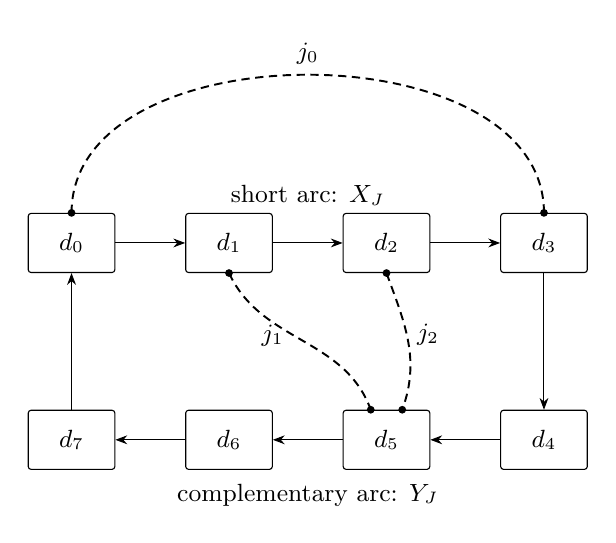
\begin{tikzpicture}[
  x=1cm,y=1cm,
  block/.style={draw,rounded corners=1pt,minimum width=1.1cm,minimum height=0.75cm,inner sep=2pt},
  word/.style={-{Stealth[length=1.5mm]},line width=0.35pt},
  equality/.style={densely dashed,line width=0.7pt},
  every node/.style={font=\small}
]
\node[block] (d0) at (0,1.5) {$d_0$};
\node[block] (d1) at (2,1.5) {$d_1$};
\node[block] (d2) at (4,1.5) {$d_2$};
\node[block] (d3) at (6,1.5) {$d_3$};
\node[block] (d4) at (6,-1) {$d_4$};
\node[block] (d5) at (4,-1) {$d_5$};
\node[block] (d6) at (2,-1) {$d_6$};
\node[block] (d7) at (0,-1) {$d_7$};

\draw[word] (d0.east) -- (d1.west);
\draw[word] (d1.east) -- (d2.west);
\draw[word] (d2.east) -- (d3.west);
\draw[word] (d3.south) -- (d4.north);
\draw[word] (d4.west) -- (d5.east);
\draw[word] (d5.west) -- (d6.east);
\draw[word] (d6.west) -- (d7.east);
\draw[word] (d7.north) -- (d0.south);

\coordinate (o51) at ($(d5.north)+(-0.2,0)$);
\coordinate (o52) at ($(d5.north)+(0.2,0)$);
\draw[equality] (d0.north) to[out=90,in=90]
  node[above,pos=0.5] {$j_0$} (d3.north);
\draw[equality] (d1.south) to[out=-65,in=110]
  node[left,pos=0.45] {$j_1$} (o51);
\draw[equality] (d2.south) to[out=-70,in=70]
  node[right,pos=0.45] {$j_2$} (o52);
\foreach \point in {d0.north,d3.north,d1.south,d2.south,o51,o52}
  \fill (\point) circle[radius=1.4pt];

\node[fill=white,inner sep=2pt] at (3,2.1) {short arc: $X_J$};
\node at (3,-1.7) {complementary arc: $Y_J$};
\end{tikzpicture}

\caption{Selected equality links in one fixed cyclic word with eight diagonal
blocks and $\ell=3$. The short arc $0\to1\to2\to3$ and its complement
indicate the positions contributing to $X_J$ and $Y_J$. The two marks in
block $5$ are distinct mate occurrences. Further occurrences and equality
links are omitted; distinct prescribed classes may use equal numerical
partition indices after inequalities between classes have been removed.}
\label{fig:shortest-pair}
\end{figure}

State Cauchy--Schwarz gives
\begin{equation}
 \left|\sum_J\varphi(X_JY_J)\right|
 \le
 \left(\sum_J\varphi(X_JX_J^*)\right)^{1/2}
 \left(\sum_J\varphi(Y_J^*Y_J)\right)^{1/2}.
 \label{eq:shortest-pair-cs}
\end{equation}
The second square sum is uniformly bounded. First drop $E_\ell'$ from
the positive operator bound for $Y_J^*Y_J$. Order the exterior mate
occurrences from left to right, using commutativity for those in one
diagonal block. Write $\mathbf j=(j_1,\ldots,j_{\ell-1})$. At the first
remaining mate occurrence, factor
\[
 B_{\mathbf j}=C_0F_jB'_{\mathbf j'},
\]
where $j$ is that occurrence's index, $\mathbf j'$ lists the others,
$\{F_j\}_j$ is its projection partition, and $C_0,B'_{\mathbf j'}$ are
independent of $j$. Then
\[
 \sum_j B_{\mathbf j}^*B_{\mathbf j}
 = {B'_{\mathbf j'}}^*
       \left(\sum_jF_jC_0^*C_0F_j\right)B'_{\mathbf j'}
 \leq\|C_0\|^2{B'_{\mathbf j'}}^*B'_{\mathbf j'}.
\]
Iterating over the remaining mate occurrences, with the fixed norm bounds
on the intervening multipliers, gives
\[
 \sum_{j_1,\ldots,j_{\ell-1}}
 B_{j_1,\ldots,j_{\ell-1}}^*
 B_{j_1,\ldots,j_{\ell-1}}
 \leq C\,1
\]
for a fixed constant $C$. When $\ell=1$, this is simply the fixed norm
bound for the exterior word. Finally sum the $E_0$ corners in the state.
As $\{\lambda_0(e_{j_0})\}_{j_0}$ is a partition in the centralizer, this
leaves a bound independent of $\mathcal P$ and of all auxiliary unitaries.

We have reduced the moment estimate to the first square sum in
Equation~\eqref{eq:shortest-pair-cs}. Its smallness will come from a
collision between the two endpoint indices. The interior pinchings
first converge at fixed coarse endpoint data; only afterward will
those coarse endpoint data be refined.

Remove $V_0$ from the state by centrality and sum the interior indices
in $X_JX_J^*$. The result is
\begin{equation}
 \sum_{j_0}
 \varphi\!\left(
   \lambda_0(e_{j_0})
   C_{\mathcal P}\bigl(\lambda_\ell(e_{j_0})\bigr)
   \lambda_0(e_{j_0})\right),
 \label{eq:endpoint-collision}
\end{equation}
where the positive map $C_{\mathcal P}:A\to M$ is given by the nested
operations
\begin{align*}
 C_{\mathcal P}(f)&=L_1,\\
 L_\ell&=y_\ell f y_\ell^*,\\
 L_h&=y_h S_{\lambda_h(\mathcal P)}
                (V_hL_{h+1}V_h^*)y_h^*
       \qquad(h=\ell-1,\ldots,1).
\end{align*}
For $\ell=1$ this means simply $C_{\mathcal P}(f)=y_1fy_1^*$.

Fix a coarse partition $\mathcal Q$ from the generating sequence and
let $\mathcal P$ refine it. Positivity permits each input projection
in Equation~\eqref{eq:endpoint-collision} to be enlarged to its coarse
piece. Regrouping the output corners by centrality then bounds that
expression by
\begin{equation}
 \sum_{e\in\mathcal Q}
 \varphi\!\left(
    \lambda_0(e)C_{\mathcal P}\bigl(\lambda_\ell(e)\bigr)
    \lambda_0(e)\right).
 \label{eq:coarse-endpoint-bound}
\end{equation}
For each fixed $f\in A$, the nested expression defining
$C_{\mathcal P}(f)$ converges in state norm to the expression in which
each pinching is replaced by $E_A$ and the $V_h$ disappear. This
convergence is uniform over the auxiliary unitaries. Indeed, work from
the innermost pinching outward. Each translated sequence
$\lambda_h(\mathcal P_j)$ is generating, so
Lemma~\ref{lem:pinching} gives its state-norm convergence to $E_A$ on
a fixed input. Conjugation by $V_h$ commutes with the pinching,
preserves the state norm, and fixes the limiting $A$-valued datum.
Pinching is contractive in the state norm. Its error can thus be
propagated through the fixed left and right multipliers $y_h,y_h^*$
using Lemma~\ref{lem:state-multipliers}, uniformly over all the
remaining phases. This proves the asserted inside-out convergence.

Define positive kernel maps on $A$ by
\[
 K_h(f)=E_A(y_hfy_h^*)\qquad(1\le h\le\ell).
\]
For each fixed input $f=\lambda_\ell(e)$, $e\in\mathcal Q$, the preceding
convergence applies. Since $\mathcal Q$ is finite, the limit of
Equation~\eqref{eq:coarse-endpoint-bound}, with $\mathcal Q$ fixed, is
\begin{equation}
 \sum_{e\in\mathcal Q}
   \int_X\lambda_0(e)
       (K_1\circ\cdots\circ K_\ell)
          \bigl(\lambda_\ell(e)\bigr)\,d\mu.
 \label{eq:coarse-kernel-collision}
\end{equation}
Proposition~\ref{prop:atomless-kernels}, applied to the adjoints of the
$y_h$, says that these kernels and their composition are atomless
almost everywhere. In taking compositions, a preceding kernel avoids
the fixed null exceptional set where a following kernel may fail to be
atomless.

Finally refine $\mathcal Q$ along the generating sequence. The
integrand sum in Equation~\eqref{eq:coarse-kernel-collision} tests
whether $\gamma_0$ of the output site and $\gamma_\ell$ of the input
site lie in the same partition piece. These conditions decrease to
equality of those two points. Since $\gamma_\ell$ is one-to-one,
this is a graph having zero conditional mass for each atomless row
of the composed kernel. Nonsingularity makes all fixed null exceptions
irrelevant. The kernel masses are bounded, so bounded convergence shows
that Equation~\eqref{eq:coarse-kernel-collision} tends to zero.

For each fixed coarse $\mathcal Q$, the limsup of the first square sum,
even after taking the supremum over the auxiliary unitaries at each
fine $\mathcal P$, was bounded by
Equation~\eqref{eq:coarse-kernel-collision}. First take that fine-partition
limsup and then refine $\mathcal Q$. The first square sum therefore
vanishes uniformly in the auxiliary phases. The second square sum was
uniformly bounded, so Equation~\eqref{eq:shortest-pair-cs} proves
vanishing of the equality-pattern sum. Averaging the auxiliary phases,
undoing the finite inclusion--exclusion and Fourier expansions, and
then removing the fixed analytic approximations proves the required
vanishing in Equation~\eqref{eq:cyclic-centered-word}. The induction
now proves Equation~\eqref{eq:moment-transfer}.
\end{proof}

The moment-transfer statement uses a fixed finite symbol alphabet.
The following approximation allows it to be applied to the measurable
color partitions supplied by Theorem~\ref{thm:bernoulli-coloring}.

\begin{lemma}[Cylinder approximation of projection partitions]
\label{lem:cylinder-partitions}
In the Bernoulli extension of Lemma~\ref{lem:bernoulli-model}, let
$p_1,\ldots,p_r\in B$ be projections with $\sum_i p_i=1$ and
$p_ip_h=0$ for $i\ne h$. For every $\delta>0$ there is a projection
partition $b_1,\ldots,b_r\in B$, each of whose members is a finite
cylinder function for one common finite dyadic symbol size, such that
\[
 \|b_i-p_i\|_\Phi<\delta\qquad(1\le i\le r).
\]
Every evaluation of this cylinder partition by the preceding
finite-symbol substitution gives a projection partition of $1$ in
$A$, modulo the fixed null sets of its definition.
\end{lemma}

\begin{proof}
The extension $\sigma$-algebra is generated by base measurable sets and
countably many label-coordinate readings along the partial graphings.
Dyadic approximations to the label coordinates therefore show that the
finite cylinder set algebra, allowing arbitrary base measurable sets,
is dense in probability. Approximate each of the measurable sets
corresponding to the $p_i$ by sets in this algebra. Disjointize the
approximations in order and put the remaining complement into one
piece, retaining exactly $r$ pieces and covering the identity. The
resulting symmetric-difference measures can be made arbitrarily small,
which gives the displayed state-norm bounds for their projections.
There are only finitely many pieces and coordinates, so all of them
use one common finite dyadic symbol size after refinement.

The resulting identities $b_i=b_i^*=b_i^2$, $b_ib_h=0$ for $i\ne h$,
and $\sum_i b_i=1$ are identities of finite cylinder functions. The
full-support argument in the construction of $\mathrm{ev}_{\mathcal P}$
shows that substitution preserves all these identities. Thus their
evaluations form a genuine projection partition in $A$.
\end{proof}

\section{Completion of the paving argument}\label{sec:completion}

We now combine the coloring theorem and moment transfer. The coloring estimates apply to finite-support approximations of a Cartan operator. Before transferring a fixed moment, we must return to the original operator without requiring a rate of approximation depending exponentially on the moment order. A clipping argument accomplishes this. Its use in a nontracial state requires the following elementary observation about varying right multipliers.

\subsection{Continuous calculus for varying sequences}

\begin{lemma}\label{lem:multiplier-calculus}
Let $\mathcal L$ be a von Neumann algebra with a faithful normal state $\omega$. Let $\mathscr R_\omega$ consist of all uniformly bounded sequences $(R_n)$ in $\mathcal L$ such that
\[
 \|D_nR_n\|_\omega\longrightarrow0
\]
whenever $(D_n)$ is uniformly bounded and $\|D_n\|_\omega\to0$. Then $\mathscr R_\omega$ is an algebra, closed for the supremum operator norm. It contains all constant sequences and all uniformly bounded sequences in the centralizer of $\omega$. It is also closed under adding uniformly bounded sequences converging to zero in $\|\cdot\|_\omega$.

If $(U_n),(V_n)\in\mathscr R_\omega$ are self-adjoint, uniformly bounded, and $\|U_n-V_n\|_\omega\to0$, then for every continuous function $f$ on a compact interval containing their spectra,
\[
 (f(U_n)),(f(V_n))\in\mathscr R_\omega,
 \qquad \|f(U_n)-f(V_n)\|_\omega\longrightarrow0.
\]
\end{lemma}

\begin{proof}
The assertions for constant sequences and centralizer sequences follow from Lemma~\ref{lem:state-multipliers}. If $(R_n),(S_n)\in\mathscr R_\omega$ and $(D_n)$ is a bounded state-norm-null sequence, then $(D_nR_n)$ is another such sequence, so $\|D_nR_nS_n\|_\omega\to0$. Addition is immediate. Closure in the supremum norm follows by approximating the right multiplier uniformly before taking the limit in $n$.

For the perturbation assertion, if $(E_n)$ is bounded and state-norm-null, then
\[
 \|D_nE_n\|_\omega\le\|D_n\|\,\|E_n\|_\omega\longrightarrow0.
\]
Thus $(R_n+E_n)\in\mathscr R_\omega$ whenever $(R_n)\in\mathscr R_\omega$.

For a polynomial $f$, the assertion about membership follows from the algebra property. Polynomial differences are controlled by the telescoping identity
\[
 U_n^j-V_n^j=\sum_{h=0}^{j-1}U_n^h(U_n-V_n)V_n^{j-1-h}.
\]
Every right multiplier on the right belongs to $\mathscr R_\omega$, while the left multipliers are uniformly bounded. Each summand therefore tends to zero in state norm. Uniform polynomial approximation on the common spectral interval proves both assertions for continuous $f$.
\end{proof}

\subsection{Paving in the presence of a central state}

\begin{proposition}\label{prop:expected}
Let $A\subseteq M$ be a masa and let $\varphi$ be a faithful normal state on $M$ with $A$ in its centralizer. For $0<\eps<1$, put
\[
 r_{\mathrm e}=\left\lceil 20000^2\eps^{-2}\right\rceil.
\]
For every self-adjoint contraction $x\in M$ and every $\rho>0$, there are a partition $P=(p_1,\ldots,p_{r_{\mathrm e}})$ in $A$ and a projection $q\in M$ such that
\[
 \varphi(1-q)<\rho,
 \qquad \|q(S_P(x)-E_Ax)q\|\le\eps.
\]
Here $E_A$ is the $\varphi$-preserving conditional expectation onto $A$.
\end{proposition}

\begin{proof}
By Lemma~\ref{lem:separable-reduction}, it suffices to work with separable predual. The conditional expectation in that reduction is the restriction of $E_A$, so proving the stated diagonal choice in the smaller inclusion proves it in the original one. We henceforth use the notation of Sections~\ref{sec:kernels} and~\ref{sec:transfer}.

Fix $r=r_{\mathrm e}$ and write
\[
 a=E_Ax,\qquad y=E_Nx-E_Ax\in N,
 \qquad w=x-E_Nx\in\ker E_N.
\]
The three elements are self-adjoint, $\|a\|\le1$, and $\|y\|,\|w\|\le2$. Moreover $E_Ay=0$: uniqueness of the $\varphi$-preserving expectation onto $A$ gives $E_AE_N=E_A$.

\paragraph{Finite-support Cartan approximations.}
Choose self-adjoint contractions in $N_{\mathrm{alg}}$ converging strongly to $E_Nx$. To obtain them, first apply Kaplansky density to the norm closure of the finite normalizer algebra, then approximate its self-adjoint contractions in norm by self-adjoint elements of $N_{\mathrm{alg}}$ and rescale. Bounded strong approximation can be taken sequentially in the faithful separable state representation.

For each approximant, only finitely many partial isomorphisms occur in its support. We may also arrange a bound on their edge Radon--Nikodym ratios. Indeed, for such a finite list of maps $\gamma$, remove from $X$ each domain set where $\Delta(\gamma v,v)$ lies outside $[b^{-1},b]$, and let $e_b\in A$ be the indicator of the remaining set. As $b\to\infty$, these projections increase strongly to $1$. Compressing the approximant by $e_b$ preserves self-adjointness and its contraction bound, and restricts every surviving edge to the required ratio range. Enlarge the finite list by its inverses if necessary. Choosing $b$ sufficiently large for each approximant preserves strong convergence.

Subtracting the diagonal now gives a sequence
\begin{equation}\label{eq:cartan-approximants}
 y_n=y_n^*\in N_{\mathrm{alg}},\qquad E_Ay_n=0,
 \qquad \|y_n\|\le2,\qquad \|y_n-y\|_\varphi\longrightarrow0.
\end{equation}
Each $y_n/2$ is represented by measurable zero-diagonal Hermitian contractions on orbit $\ell^2$ spaces, supported on an undirected graph of finite degree with bounded edge cocycle ratios. These bounds may depend on $n$. Theorem~\ref{thm:bernoulli-coloring} permits this dependence: it does not affect $r$.

\paragraph{One partition for the two operator terms.}
Use the fixed relative Bernoulli extension $\widetilde N$ and amalgamated product
\[
 \mathcal K=M*_N\widetilde N,
 \qquad \Phi=\varphi|_N\circ E_N^{\mathcal K},
\]
from Lemma~\ref{lem:bernoulli-model}. Apply Theorem~\ref{thm:bernoulli-coloring} to $y_n/2$ with
\begin{equation}\label{eq:coloring-parameters}
 t=\frac4{\sqrt r},\qquad \alpha=\frac\eps{32},
 \qquad m=n,\qquad \eta=\left(\frac\eps{16}\right)^{2n}.
\end{equation}
Denote the color projections by $p_1^n,\ldots,p_r^n\in B$. They form a partition, belong to the centralizer of $\Phi$, and satisfy
\begin{equation}\label{eq:color-marginals-completion}
 \widetilde E_N(p_i^n)=r^{-1}1\qquad(1\le i\le r).
\end{equation}
With $\beta=80$, the norm bound supplied by the coloring theorem, after restoring the factor two, obeys
\begin{equation}\label{eq:cartan-numerical-bound}
 2(2\beta t+\alpha)=\frac{1280}{\sqrt r}+\frac\eps{16}
 \le\frac{253}{2000}\eps<\frac\eps4.
\end{equation}

Put
\[
 \widehat Y_n=\sum_{i=1}^r p_i^n y_n p_i^n\in\widetilde N.
\]
At a root where the radius-$n$ ball has the asserted pinching bound, $\widehat Y_n^n$ applied to the root vector agrees with the $n$th power of that principal matrix applied to the same vector. Every path of length $n$ starting at the root stays in its radius-$n$ ball. At all other roots, $\|\widehat Y_n\|\le2$. Integrating the squared norms of these vectors gives
\begin{equation}\label{eq:cartan-high-moment}
 \Phi(\widehat Y_n^{2n})
 \le\left(\frac\eps4\right)^{2n}
       +2^{2n}\left(\frac\eps{16}\right)^{2n}.
\end{equation}
This uses diagonal integration in the relation representation, not a trace on the nonsingular relation algebra.

For the original operators set
\[
 Y_n=\sum_{i=1}^r p_i^n y p_i^n,
 \qquad W_n=\sum_{i=1}^r p_i^n w p_i^n.
\]
Pinching by a centralizer partition is contractive in the state norm, so Equation~\eqref{eq:cartan-approximants} implies
\begin{equation}\label{eq:pinched-approximation}
 \|Y_n-\widehat Y_n\|_\Phi\longrightarrow0.
\end{equation}
By Lemma~\ref{lem:free-compression} and Equation~\eqref{eq:color-marginals-completion},
\begin{equation}\label{eq:free-numerical-bound}
 \|W_n\|\le2\left(\frac1r+\frac2{\sqrt r}\right)
 \le\frac{40001}{200000000}\eps<\frac\eps4.
\end{equation}
Here orthogonality of the $p_i^n$ makes the norm of the block sum the maximum of its block norms. Thus the same $r$ projections control the complementary term; there is no second partition refinement.

\paragraph{Clipping before fixing a transferred moment.}
Let $f:\mathbb R\to[-\eps/2,\eps/2]$ be the continuous clipping function
\[
 f(s)=\max\{-\eps/2,\min\{s,\eps/2\}\}.
\]
Spectral calculus and Equation~\eqref{eq:cartan-high-moment} show that
\[
 \Phi\bigl(1_{\{|\widehat Y_n|>\eps/2\}}\bigr)
 \le\left(\frac2\eps\right)^{2n}\Phi(\widehat Y_n^{2n})
 \le2^{-2n}+4^{-2n}.
\]
Since $\|\widehat Y_n\|\le2$, it follows that
\begin{equation}\label{eq:approximate-clipping}
 \|\widehat Y_n-f(\widehat Y_n)\|_\Phi\longrightarrow0.
\end{equation}

We apply Lemma~\ref{lem:multiplier-calculus} in $\mathcal K$. Each sequence $(p_i^n)$ lies in $\mathscr R_\Phi$, and $r$ is fixed. Hence $(Y_n)$ and $(W_n)$ belong to that algebra, being finite sums of products of centralizer sequences and fixed operators. Equation~\eqref{eq:pinched-approximation} also places $(\widehat Y_n)$ in it. Equations~\eqref{eq:pinched-approximation}--\eqref{eq:approximate-clipping} and the continuous-calculus conclusion of the lemma yield
\begin{equation}\label{eq:original-clipping}
 \|Y_n-f(Y_n)\|_\Phi\longrightarrow0.
\end{equation}

The self-adjoint operators
\[
 Z_n=Y_n+W_n=\sum_{i=1}^r p_i^n(x-a)p_i^n
\]
therefore differ by a bounded state-norm-null sequence from
\[
 Q_n=f(Y_n)+W_n,\qquad \|Q_n\|\le\frac{3\eps}{4}.
\]
Both sequences belong to $\mathscr R_\Phi$. For every fixed integer $k\ge1$, telescoping their powers gives
\begin{equation}\label{eq:fixed-model-moment}
 \limsup_{n\to\infty}\Phi(Z_n^{2k})
 \le\left(\frac{3\eps}{4}\right)^{2k}.
\end{equation}
Only a fixed power is used at this stage. In particular, Equation~\eqref{eq:cartan-approximants} required no prescribed rate of convergence.

\paragraph{Transfer and the final spectral cut.}
Fix $\rho>0$. First choose $k$ so large that $(3/4)^{2k}<\rho/4$. Then choose $n$ sufficiently large in Equation~\eqref{eq:fixed-model-moment} that
\[
 \Phi(Z_n^{2k})<\frac\rho2\eps^{2k}.
\]
With $n$ and $k$ fixed, approximate the partition $(p_i^n)$ in $B$ by a finite-symbol cylinder partition, using Lemma~\ref{lem:cylinder-partitions}. Bounded state-norm approximation of these self-adjoint projections is strong-* approximation, so the fixed polynomial moment changes arbitrarily little. We may retain the strict upper bound $\rho\eps^{2k}$ with positive slack.

Proposition~\ref{prop:moment-transfer} applies to the expansion of this moment. For a sufficiently fine base partition, its averaged evaluated moment remains strictly less than $\rho\eps^{2k}$. Every evaluation is a genuine projection partition in $A$, and its even moment is nonnegative. Some deterministic evaluation consequently gives a partition $P=(p_1,\ldots,p_r)$ with
\[
 \varphi\left(\left[\sum_{i=1}^r p_i(x-a)p_i\right]^{2k}\right)
 <\rho\eps^{2k}.
\]
Let $z=\sum_i p_i(x-a)p_i=z^*$ and take $q=1_{[-\eps,\eps]}(z)\in M$. Then
\[
 \varphi(1-q)\le\eps^{-2k}\varphi(z^{2k})<\rho,
 \qquad \|qzq\|\le\eps.
\]
Because $a\in A$ commutes with the partition, $z=S_P(x)-a$. This proves the proposition with the number of colors fixed before $\rho$.
\end{proof}

\subsection{Arbitrary inclusions}

\begin{proof}[Proof of Theorem~\ref{thm:main}]
If $x=0$, take $p_1=1$, $p_2=\cdots=p_{r_\eps}=0$, $a=0$, and $q=1$. Otherwise replace $x$ by $x/\|x\|$. Proposition~\ref{prop:expected}, together with Proposition~\ref{prop:state-reduction}, supplies the required paving in the original representation using
\[
 r=\left\lceil400000000\eps^{-2}\right\rceil
      +\left\lceil4/\eps\right\rceil+1
\]
projections. This number depends only on $\eps$. The supporting corner and all partitions, diagonal elements, and compression projections may depend on $F$ and $\delta$, as permitted in Definition~\ref{def:so-paving}. The construction has diagonal norm at most one, and
\[
 r\le400000000\eps^{-2}+4\eps^{-1}+3
 \le400000007\eps^{-2}<500000000\eps^{-2}.
\]
Multiplying the diagonal by the original $\|x\|$ restores scale and gives every assertion of Theorem~\ref{thm:main}.
\end{proof}

\begin{thebibliography}{MSS15}
\raggedright

\bibitem[AS12]{AS12}
Charles A. Akemann and David Sherman,
\emph{Conditional expectations onto maximal abelian star-subalgebras},
Journal of Operator Theory \textbf{68} (2012), no.~2, 597--607.
\href{https://jot.theta.ro/jot/archive/2012-068-002/2012-068-002-013.pdf}{Published article}.

\bibitem[Ara74]{Ara74}
Huzihiro Araki,
\emph{Some properties of modular conjugation operator of von Neumann algebras and a non-commutative Radon--Nikodym theorem with a chain rule},
Pacific Journal of Mathematics \textbf{50} (1974), no.~2, 309--354.
\href{https://msp.org/pjm/1974/50-2/pjm-v50-n2-p02-p.pdf}{Published article}.

\bibitem[FM77]{FM77}
Jacob Feldman and Calvin C. Moore,
\emph{Ergodic equivalence relations, cohomology, and von Neumann algebras. II},
Transactions of the American Mathematical Society \textbf{234} (1977), 325--359.
\href{https://doi.org/10.1090/S0002-9947-1977-0578730-2}{doi:10.1090/S0002-9947-1977-0578730-2}.

\bibitem[Haa75]{Haa75}
Uffe Haagerup,
\emph{The standard form of von Neumann algebras},
Mathematica Scandinavica \textbf{37} (1975), 271--283.
\href{https://doi.org/10.7146/math.scand.a-11606}{doi:10.7146/math.scand.a-11606}.

\bibitem[Haa79]{Haa79}
Uffe Haagerup,
\emph{$L^p$-spaces associated with an arbitrary von Neumann algebra},
in \emph{Alg\`ebres d'op\'erateurs et leurs applications en physique math\'ematique}
(Marseille, 1977), Colloques Internationaux du C.N.R.S. \textbf{274},
C.N.R.S., Paris, 1979, pp.~175--184.
\href{https://math.berkeley.edu/~pavlov/scans/haagerup.pdf}{Original paper}.

\bibitem[KR86]{KR86}
Richard V. Kadison and John R. Ringrose,
\emph{Fundamentals of the Theory of Operator Algebras},
Vol.~II: \emph{Advanced Theory}, Pure and Applied Mathematics \textbf{100},
Academic Press, Orlando, FL, 1986.
\href{https://shop.elsevier.com/books/fundamentals-of-the-theory-of-operator-algebras-v2/kadison/978-0-12-393302-7}{Publisher information}.

\bibitem[Kec95]{Kec95}
Alexander S. Kechris,
\emph{Classical Descriptive Set Theory},
Graduate Texts in Mathematics \textbf{156}, Springer-Verlag, New York, 1995.
\href{https://doi.org/10.1007/978-1-4612-4190-4}{doi:10.1007/978-1-4612-4190-4}.

\bibitem[Mah64]{Mah64}
Dorothy Maharam,
\emph{Incompressible transformations},
Fundamenta Mathematicae \textbf{56} (1964), no.~1, 35--50.
\href{https://doi.org/10.4064/fm-56-1-35-50}{doi:10.4064/fm-56-1-35-50}.

\bibitem[MSS15]{MSS15}
Adam W. Marcus, Daniel A. Spielman, and Nikhil Srivastava,
\emph{Interlacing families II: Mixed characteristic polynomials and the Kadison--Singer problem},
Annals of Mathematics (2) \textbf{182} (2015), no.~1, 327--350.
\href{https://doi.org/10.4007/annals.2015.182.1.8}{doi:10.4007/annals.2015.182.1.8}.

\bibitem[Ope26]{ApproxCompanion26}
OpenAI,
\emph{Approximation Paving over Arbitrary Maximal Abelian Subalgebras},
OpenAI Math Release preprint
\href{https://github.com/openai/math/blob/main/preprints/Approximation-Paving-over-Arbitrary-Maximal-Abelian-Subalgebras-September-25-2026/Approximation-Paving-over-Arbitrary-Maximal-Abelian-Subalgebras-September-25-2026.pdf}{OAI:Approximation-Paving-over-Arbitrary-Maximal-Abelian-Subalgebras-September-25-2026},
2026, Theorem~1.1.

\bibitem[Pop14]{Popa14}
Sorin Popa,
\emph{A $\mathrm{II}_1$ factor approach to the Kadison--Singer problem},
Communications in Mathematical Physics \textbf{332} (2014), 379--414.
\href{https://doi.org/10.1007/s00220-014-2055-4}{doi:10.1007/s00220-014-2055-4}.

\bibitem[PV15]{PV15}
Sorin Popa and Stefaan Vaes,
\emph{Paving over arbitrary MASAs in von Neumann algebras},
Analysis \& PDE \textbf{8} (2015), no.~4, 1001--1023.
\href{https://doi.org/10.2140/apde.2015.8.1001}{doi:10.2140/apde.2015.8.1001}.

\bibitem[PV16]{PV16}
Sorin Popa and Stefaan Vaes,
\emph{On the optimal paving over MASAs in von Neumann algebras},
Contemporary Mathematics \textbf{671} (2016), 199--208.
\href{https://doi.org/10.1090/conm/671/13511}{doi:10.1090/conm/671/13511}.

\bibitem[PS70]{PS70}
Robert T. Powers and Erling St{\o}rmer,
\emph{Free states of the canonical anticommutation relations},
Communications in Mathematical Physics \textbf{16} (1970), 1--33.
\href{https://doi.org/10.1007/BF01645492}{doi:10.1007/BF01645492}.

\bibitem[RS17]{RS17}
Mohan Ravichandran and Nikhil Srivastava,
\emph{Asymptotically optimal multi-paving},
International Mathematics Research Notices \textbf{2021} (2021), no.~14, 10908--10940.
\href{https://doi.org/10.1093/imrn/rnz111}{doi:10.1093/imrn/rnz111};
numbered theorem locators refer to \href{https://arxiv.org/abs/1706.03737v2}{arXiv:1706.03737v2}.

\bibitem[RS06]{RoySamorodnitsky06}
Parthanil Roy and Gennady Samorodnitsky,
\emph{Maharam extension for nonsingular group actions},
2006, \href{https://arxiv.org/abs/math/0611891v1}{arXiv:math/0611891v1}.

\bibitem[Tak72]{Tak72}
Masamichi Takesaki,
\emph{Conditional expectations in von Neumann algebras},
Journal of Functional Analysis \textbf{9} (1972), no.~3, 306--321.
\href{https://doi.org/10.1016/0022-1236(72)90004-3}{doi:10.1016/0022-1236(72)90004-3}.

\bibitem[Ued99]{Ued99}
Yoshimichi Ueda,
\emph{Amalgamated free product over Cartan subalgebra},
Pacific Journal of Mathematics \textbf{191} (1999), no.~2, 359--392.
\href{https://doi.org/10.2140/pjm.1999.191.359}{doi:10.2140/pjm.1999.191.359}.

\bibitem[Ued13]{Ued13}
Yoshimichi Ueda,
\emph{Some analysis of amalgamated free products of von Neumann algebras in the non-tracial setting},
Journal of the London Mathematical Society (2) \textbf{88} (2013), no.~1, 25--48.
\href{https://doi.org/10.1112/jlms/jds081}{doi:10.1112/jlms/jds081}.

\end{thebibliography}

\end{document}
